
\documentclass{createspace}

\input{00-meta-latex/shortcuts}

\usepackage{comment}
\includecomment{comment}

% forced by -output-directory option in makefile
% see https://tex.stackexchange.com/a/564296
\usepackage{etoolbox}
\makeatletter
\patchcmd\imki@putindex
  {\imki@exec{\imki@program \imki@options #1.idx}}
  {\imki@exec{cd ../build;\imki@program\imki@options#1.idx}}
  {\message{Patch succeeded in imki@putindex}}
  {\errmessage{Patch failed in imki@putindex}}
\makeatother
\makeindex[title=Skorowidz]
\makeindex[name=persons,title=Indeks osób]

\usepackage{enumitem}
\usepackage{booktabs}
\usepackage{longtable}
\usepackage[table]{xcolor}
\usepackage[colorinlistoftodos,prependcaption]{todonotes}
\usepackage{tikz}
\usetikzlibrary{arrows.meta}
\usetikzlibrary{decorations.markings}
\usetikzlibrary{decorations.pathreplacing}
\usetikzlibrary{knots}
\colorlet{darkblue}{blue!80!black}
\definecolor{diagramfiller}{RGB}{255, 182, 193} % HTML: LightPink
\definecolor{first_colour}{RGB}{255, 105, 180}
\input{00-meta-latex/diagrams}

\definecolor{hotpink}{RGB}{255, 105, 180}
\definecolor{mediumvioletred}{RGB}{199, 21, 133}
\let\oldtabular\tabular % alternate rowcolors for all tables
\let\endoldtabular\endtabular
\renewenvironment{tabular}
{\rowcolors{2}{white}{hotpink}\oldtabular}
{\endoldtabular}
\let\oldlongtable\longtable % alternate rowcolors for all long-tables
\let\endoldlongtable\endlongtable
\renewenvironment{longtable}
{\rowcolors{2}{white}{hotpink}\oldlongtable}
{\endoldlongtable}

\hypersetup{
    colorlinks,
    linkcolor={mediumvioletred},
    citecolor={mediumvioletred},
    urlcolor={mediumvioletred}
}

\author{Casimir Allard}
\title{Kombinatoryczna teoria węzłów}

\begin{document}


\input{include/head_1}
\input{include/head_2}
\input{include/head_3}

% strona czwarta

\thispagestyle{empty}
\begin{figure}[H]
\begin{minipage}[b]{.48\linewidth}
{\noindent Prof. Casimir Allard\\
Université Bordeaux I\\
351 Cours de la Libération\\
33400 Talence, Francja}
\end{minipage}
\begin{minipage}[b]{.48\linewidth}
{\noindent Adélaïde Gauthier\\
École polytechnique\\
Route de Saclay\\
91128 Palaiseau, Francja}
\end{minipage}
\end{figure}

{\noindent \textbf{Kategorie MSC 2020}\\57K10 (niskowymiarowa teoria węzłów),\\57K30 (topologia 3-rozmaitości)} \vspace{5mm}

{\noindent \textbf{Tytuł oryginału}\\La théorie combinatoire des næuds}
\vspace{5mm}

{\noindent \textbf{Z francuskiego przetłumaczyła}\\Charlotte Ocelot} 
\vspace{5mm}

{\noindent \textbf{Okładkę zaprojektował}\\Raphaël Embusqueur}
\vspace{5mm}

{\noindent \textbf{Zredagował}\\Gniewomir Grzywiasty}
\vspace{5mm}

{\noindent \textbf{Zredagowała technicznie}\\Jagoda Kłos}
\vspace{5mm}

{\noindent \textbf{Złożyli i połamali}\\Porte de Versailles, Paryż}
\vspace{5mm}

{\noindent \textbf{Korekty dokonali}\\Ignacy Filemon, Gabriel Bonifacy}

\vfill

{\noindent Copyleft © 2024 by Antykwariat Czarnoksięski.
Książka, a żeby było śmieszniej także każda jej część, mogą być przedrukowywane oraz w jakikolwiek inny sposób reprodukowane czy powielane mechanicznie, fotooptycznie, zapisywane elektronicznie lub magnetycznie, oraz odczytywane w środkach publicznego przekazu bez pisemnej zgody wydawcy.
}

\vspace{5mm}
{
    \noindent
    Tekst udostępniany na licencji Creative Commons: uznanie autorstwa, użycie niekomercyjne. Przeczytaj więcej na \url{https://creativecommons.org/licenses/by-nc/4.0/deed.pl}.
}

\vspace{5mm}

{\noindent Przygotowano w systemie \TeX, wydrukowano na siarczystym papierze.}

% koniec strony czwartej



% strona piąta

\chapter*{Przedmowa}
Książka wprowadza we współczesną teorię węzłów, najważniejsze metody i obszary tej wciąż niedocenianej, choć żywo rozwijającej się dyscypliny matematycznej.
Tor wykładu wzorowany jest na seminarium z teorii węzłów jakie odbyło się na Wydziale Matematyki Uniwersytetu Wrocławskiego w semestrze zimowym 2013/2014 i dlatego podręcznik nadaje się szczególnie do pierwszego czytania dla studentów wyższych lat studiów matematycznych, natomiast dla młodych pracowników naukowych może okazać się pożytecznym źródłem odsyłaczy do prac, które zainspirują do dalszych badań.
Zwięźle i na tyle, na ile było to możliwe opisuję rozmaite narzędzia stosowane do badania węzłów, splotów, supłów i innych: klasyczne niezmienniki numeryczne i ruchy Reidemeistera, niezmienniki kolorujące i spokrewnione z nimi kwandle, potem diagramatyczny wielomian Jonesa, homologiczny wielomian Alexandera oraz dość świeże niezmienniki typu skończonego.
Ze względu na niepełne zrozumienie maszynerii topologi algebraicznej, rozdział czwarty został napisany trochę niechlujnie, jednakże żywię nadzieję poprawić się w następnym wydaniu trzymanej przez Ciebie książki.
W ostatnim, piątym rozdziale przedstawiam krótko charakterystyczne rodziny: warkocze, dwumostowe sploty, mutanty, precle, sploty torusowe, satelitarne i hiperboliczne, wreszcie węzły plastrowe i taśmowe, obiekt zainteresowań czterowymiarowej topologii.
Dołączam również tablice węzłów pierwszych o małej liczbie skrzyżowań.
Z takim zakresem i ujęciem materiału pozycja jest unikalna nie tylko we francuskiej, ale i w światowej literaturze matematycznej.

Serdecznie dziękuję Ś. G. oraz J. Ś. bez których ten tekst nigdy by nie powstał.

\begin{flushright}
Casimir Allard,\\Marsylia, 4 lutego 2019
\end{flushright}

\newpage
\section*{Przedmowa do wydania drugiego}
Od poprzedniego wydania minął ponad rok i~trochę się w~tym czasie zmieniło.

Dodałem informację o~różnych notacjach dla węzłów, poprawiłem informację na temat płci niektórych osób, napisałem nową sekcję o~macierzy Seiferta, wymieniłem niezmienniki nieodróżniające mutantów.
Pojawiła się klasyfikacja kwandli, nierówność Mortona, homologia Floera i kilka mniejszych matematycznych obiektów.
Niektóre istniejące sekcje przeniosłem w~lepsze mam nadzieję miejsca, niektóre trudne dowody otrzymały swój zarys.
Tam, gdzie to możliwe, podałem rys historyczny, na przykład w~sekcji o~kolorowaniach wspomniałem o~Foxie, który chciał uczynić teorię węzłów prostszą dla swoich studentów.
Na końcu książki umieściłem krótki słowniczek angielsko-polski.
Wreszcie usunąłem znalezione literówki i~uzupełniłem luki, zarówno w~bibliografii jak i~rysunkach.
Poprawiłem drobnie typografię, dla przykładu od teraz wszystkie równania powinny być numerowane.

Żywię nadzieję, że korzystanie z~książki będzie równie (jeśli nie bardziej) przyjemne, co w~przypadku pierwszego jej wydania.

\begin{flushright}
Casimir Allard,\\Marsylia, 19 sierpnia 2020
\end{flushright}

\section*{Przedmowa do wydania trzeciego}
Lata mijały, wiele wody upłynęło w Loarze, a~wydania trzeciego wciąż nie było widać na horyzoncie.
Głównym winowajcą jest tutaj Amazon, który z~niejasnych dla mnie powodów przestał wspierać język francuski.
Pomimo przeciwności losu nie zapomniałem jednak o miłośnikach teorii węzłów i~nie przestawałem pracować w domowym zaciszu nad książką.
Nieznacznie rozrosła się ze 114 stron w 2020 roku do 1XX stron teraz, kiedy oddaję ją do druku.
Cytowań już wcześniej było bez liku (dokładniej: 240), a~teraz jest ich jeszcze więcej (aż 437).
Autor był sam jak paluch, a teraz jest nas dwoje!
% TODO: to jest licząc ostatnią stronę 5. rozdziału
Staraliśmy się nie zmieniać znacząco układu, w~myśl dewizy, że lepsze jest wrogiem dobrego.
Zupełnych nowości jest tyle, co kot napłakał.
W rozdziale drugim na osobną sekcję zasłużyły sobie etykietowania.
Natomiast w całej książce długie bloki tekstu zostały podzielone na sekcji i podsekcje tak, że odnajdywanie potrzebnych informacji w pośpiechu powinno sprawiać mniej trudu.
Z czystej przyzwoitości wymieniamy też, czego nie ma (i raczej szybko nie będzie):
\begin{enumerate}
    \item \textbf{chirurgii Dehna}.
    \item \textbf{niezmienników Reszetichina-Turajewa}.
    (Wspominamy o nich raz, za definicją \ref{def:jones_polynomial}.)
    \item \textbf{rachunku Kirby'ego}.
    Każdą zamkniętą, orientowalną 3-rozmaitość można otrzymać wykonując chirurgię Dehna na sferze wzdłuż pewnego splotu. Robion Kirby udowodnił około 1978 roku, że dwie takie rozmaitości są homeomorficzne wtedy i tylko wtedy, gdy między odpowiadającymi im splotami można przejść ruchami Kirby'ego.
    (Porównaj to ze sformułowaniem twierdzenia Reidemeistera).
    % Kirby, Robion (1978). "A calculus for framed links in S3". Inventiones Mathematicae. 45 (1): 35–56. Bibcode:1978InMat..45...35K. doi:10.1007/BF01406222. MR 0467753. S2CID 120770295. ?
    % TODO: Yanga-Baxtera?
\end{enumerate}
I to by było na tyle.
\begin{flushright}
    Casimir Allard i Adélaïde Gauthier,\\Bordeaux, \today
\end{flushright}

\section*{Przedmowa do wydania czwartego?}

Wydanie czwarte prawdopodobnie nigdy nie powstanie.
Dlaczego nam nie wyszło? 
Myślimy, że powodów da się wymienić wiele.
Opuściliśmy środowisko akademickie, zapał już teraz jest trochę słomiany i wypala się z każdym nowym pracodawcą szybciej i szybciej.
My nie do końca sprawdziliśmy się jako matematycy, a was nie można nazwać wzorowymi czytelnikami -- ale było warto!
Stworzyliśmy kilka cudownych akapitów godynch zapamiętania.
I nie wiem jak wy, ale my się naprawdę dobrze bawiliśmy.
Dziękujemy wszystkim, którzy zgłosili choć jedną uwagę i ożywili jakoś treść, ale w szczególności wdzięczni jesteśmy A. W. W., która nigdy tego nie przeczyta i której nikt tu nie zna, ale bez której nie powstałaby tak dziwna publikacja.

\begin{flushright}
Casimir Allard i Adélaïde Gauthier,\\gdzieś, kiedyś
\end{flushright}

% koniec strony piątej


\tableofcontents

\chapter{Preludium}
\input{10-introduction/100-intro}

\section{Węzły i~sploty}
Wprowadzamy pojęcia węzła i splotu, fundamentalnych obiektów teorii, o której napisana została ta książka.
Oprócz tego podajemy definicję, kiedy dwa węzły lub sploty uznajemy za tożsame oraz uzasadniamy, dlaczego akurat ta definicja jest właściwa.

Istnieją odnogi teorii węzłów, które badają inne, pokrewne obiekty.
Mamy na przykład węzły obramowane:

% DICTIONARY;framed;obramowany;węzeł
% GLOSSAIRE;framed;encadré;węzeł
% DICTIONARY;framing;obramowanie;-
% GLOSSAIRE;encadrement;obramowanie;-
\begin{definition}[obramowanie]
\index{obramowanie|see {węzeł obramowany}}%
\index{węzeł!obramowany}%
    Każde nieznikające normalne pole wektorowe $V$ na splocie $L$ nazywamy jego obramowaniem.
    Szczególnie interesujący jest przypadek, gdy wszystkie wektory tego pola są równoległe do płaszczyzny, na której leży diagram tego splotu.
\end{definition}

% DICTIONARY;virtual;wirtualny;węzeł
% GLOSSAIRE;virtuel;wirtualny;węzeł
% DICTIONARY;welded;zespawany;węzeł
% GLOSSAIRE;soudé;zespawany;węzeł
% DICTIONARY;long;długi;węzeł
% GLOSSAIRE;long;długi;węzeł
Są jeszcze węzły wirtualne, zespawane (iloraz węzłów wirtualnych przez ruch znany jako ,,nadskrzyżowania komutują''), długie (gdzie końce nie są ze sobą zszyte, ale umieszczone tak daleko, że są nieosiągalne) i inne.
% http://katlas.math.toronto.edu/ester/weldedknots/explanations.html => because the "overcrossings commute" move is not symmetric
\index{węzeł!wirtualny}%
\index{węzeł!zespawany}%
\index{węzeł!długi}%
Ta książka nie zawiera zbyt wiele informacji o wspomnianych bytach.

\subsection{Węzły}
Matematyczne węzły można traktować jako model elastycznej oraz pozbawionej grubości liny, której luźne końce zostały ze sobą połączone.
Sugeruje to przyjęcie naiwnej definicji:

\begin{definition}[węzeł (prawie)]
\index{węzeł}%
    Ciągłe oraz różnowartościowe odwzorowanie $S^1 \to \R^3$ nazywamy węzłem.
\end{definition}

Takie rozwiązanie nie jest doskonałe, ponieważ oprócz pożądanych (cokolwiek to znaczy) węzłów, obejmuje wiele innych, patologicznych obiektów takich jak ten z~rysunku \ref{fig_wild_knot}.

\begin{figure}[H]
    \centering
\begin{comment}
    \includegraphics[height=0.14\linewidth]{wild_knot.png}
\end{comment}
    \caption[caption-wild-knot]{Węzeł dziki, źródło: Wikimedia{\footnotemark}.}
\index{węzeł!dziki}%
\label{fig_wild_knot}%
\end{figure}
\footnotetext{\url{https://upload.wikimedia.org/wikipedia/commons/2/2f/Wildknot.svg}}

Zamiast wyjaśnić, jakie są jego niepożądane właściwości, podamy od razu dobrą definicję.

\begin{definition}[węzeł]
    Różnowartościowe włożenie $S^1 \to \R^3$, którego pochodna istnieje wszędzie i~nie znika nigdzie, nazywamy węzłem.
\end{definition}

% DICTIONARY;knot;węzeł;-
% GLOSSAIRE;nœud;węzeł;-
% DICTIONARY;tame;poskromiony;węzeł
% GLOSSAIRE;lisse/régulier;poskromiony;węzeł
% DICTIONARY;wild;dziki;węzeł
% GLOSSAIRE;sauvages;dziki;węzeł
\begin{definition}[węzeł]
\index{węzeł!poskromiony}%
\label{def:knot}%
    Gładkie włożenie $S^1 \hookrightarrow \R^3$ otaczająco izotopijne z~zamkniętą łamaną bez samoprzecięć nazywamy węzłem poskromionym.
    Dwa węzły są równoważne, jeśli istnieje pomiędzy nimi izotopia otaczająca.
\end{definition}

Czasami wygodniej jest rozpatrywać węzeł jako włożenie $S^1 \hookrightarrow S^3$ albo dopuścić do myśli węzły nieposkromione.
Ale jeśli nie zaznaczono inaczej, nie robimy tego: pisząc węzeł mamy na myśli poskromione włożenie w przestrzeń $\R^3$, nie $S^3$.

Potrzeba jeszcze matematycznego opisu manipulacji, jakim możemy poddawać sznur trzymany w~ręce.
Izotopia jest niewłaściwym narzędziem do tego celu: powiedzielibyśmy, że dwa węzły $K_1, K_2$ sa izotopijne, jeśli istnieje ciągła funkcja
\begin{equation}
    F \colon S^1 \times [0, 1] \to \R^3
\end{equation}
taka, że $K_1 = F(-, 0)$ jest pierwszym, zaś $K_2 = F(-,1)$ drugim węzłem (funkcję $F$ nazywa się izotopią).
Tym razem źródło problemów można wskazać jawnie.
Dowolny zaplątany fragment z węzła można usunąć wykonując sztuczkę Alexandera (ponieważ jak powiedziałyby mądre głowy, ,,przestrzeń homeomorfizmów dysku w siebie $D^{n+1} \to D^{n+1}$, które zgadzają się z odwzorowaniem tożsamościowym na brzegu dysku -- sferze $S^n$, jest spójna''):
\index[persons]{Alexander, James}%
\index{sztuczka!Alexandera}%

\begin{comment}
\begin{figure}[H]
    \centering
    \fbox{\begin{minipage}[b]{.12\linewidth}
        \centering
        \includegraphics[width=\linewidth]{../data/alexander-trick/0.png}
        \subcaption{$t = 0$}
    \end{minipage}}\,\,
    \fbox{\begin{minipage}[b]{.12\linewidth}
        \centering
        \includegraphics[width=\linewidth]{../data/alexander-trick/1.png}
        \subcaption{$t = 1/4$}
    \end{minipage}}\,\,
    \fbox{\begin{minipage}[b]{.12\linewidth}
        \centering
        \includegraphics[width=\linewidth]{../data/alexander-trick/2.png}
        \subcaption{$t=1/2$}
    \end{minipage}}\,\,
    \fbox{\begin{minipage}[b]{.12\linewidth}
        \centering
        \includegraphics[width=\linewidth]{../data/alexander-trick/3.png}
        \subcaption{$t=3/4$}
    \end{minipage}}\,\,
    \fbox{\begin{minipage}[b]{.12\linewidth}
        \centering
        \includegraphics[width=\linewidth]{../data/alexander-trick/4.png}
        \subcaption{$t = 1$}
    \end{minipage}}
    \caption[caption-alexander-trick]{Sztuczka Alexandera}
\end{figure}
\end{comment}

W podobny sposób moglibyśmy przekształcić dowolny węzeł w~niewęzeł.
Teoria, w~której wszystkie obiekty są takie same, nie jest zbyt ciekawa.
Od izotopii należy wymagać gładkości albo lokalnej płaskości,
% https://math.stackexchange.com/questions/1311865/equivalence-of-knots-ambient-isotopy-vs-homeomorphism
co zdaje się prowadzić do pojęcia izotopii otaczającej, która uwzględnia nie tylko sam węzły, ale też to, jak leżą w otaczającej je przestrzeni.

% DICTIONARY;isotopy;izotopia;-
% GLOSSAIRE;isotopie;izotopia;-
% DICTIONARY;ambient;otaczająca;izotopia
% GLOSSAIRE;ambiante;otaczająca;izotopia
\begin{definition}[izotopia otaczająca]
\index{izotopia otaczająca}%
    Niech $K_1, K_2 \colon N \hookrightarrow M$ będą włożeniami dwóch rozmaitości $N, M$.
    Ciągłe odwzorowanie $F \colon M \times [0,1] \to M$ spełniające następujące warunki:
    \begin{enumerate}
        \item funkcja $F(-, 0)$ jest odwzorowaniem tożsamościowym,
        \item każda z~funkcji $F(-, t)$ jest homeomorfizmem,
        \item złożenie $F(-, 1)$ z~pierwszym włożeniem $K_1$ daje drugie włożenie $K_2$
    \end{enumerate}
    nazywamy izotopią otaczającą przenoszącą włożenie $K_1$ na $K_2$.
\end{definition}

W~topologii rozważa się włożenia dowolnych rozmaitości, nam wystarczy jeden szczególny przypadek $N = S^1$ oraz $M = \R^3$.
Intuicyjnie, funkcja $F$ zniekształca przestrzeń $\R^3$ tak, że w~chwili początkowej $t = 0$ widzimy pierwszy, zaś w~chwili końcowej $t = 1$ drugi węzeł.
Izotopia otaczająca nie pozwala na ściąganie zaplątanych fragmentów do punktu.

Formalnie węzły to pewne odwzorowania, więc prawidłowym sposobem na zapisanie, że są izotopijne (czyli dla nas: równe), jest $K_1 \cong K_2$.
Ponieważ nie prowadzi to do problemów, będziemy jednak stosować zapis $K_1 = K_2$.
Jednocześnie często węzeł jako odwzorowanie nie będzie odróżniany od obrazu tego odwzorowania.

Istnieje jeszcze jedna, konkurencyjna definicja węzłów równoważnych:

\begin{proposition}
\label{def:equivalent_knots_2}%
    Dwa węzły są równoważne wtedy i~tylko wtedy, gdy jeden z~nich jest obrazem drugiego przez zachowujący orientację homeomorfizm $\R^3 \to \R^3$.
\end{proposition}

\begin{proof}
    Podany niżej dowód pochodzi z~książki ,,Topology from the differentiable viewpoint'' Johna Milnora.
\index[persons]{Milnor, John}%
    Musimy pokazać, że dyfeomorfizm $f \colon \R^m \to \R^m$ jest gładko izotopijny z~identycznością.
    Translacje są izotopiami, więc bez straty ogólności zakładamy, że $f(0) = 0$.
    Pochodna $f$ w~zerze jest dana wzorem $\mathrm{d}f_0(x) = \lim_{t \to 0} f(tx) /t$, więc
    \begin{equation}
        F(x, t) = \begin{cases}
            \mathrm{d}f_0(x) & t = 0 \\
            f(tx) / t & 0 < t \le 1
        \end{cases} .
    \end{equation}
    stanowi naturalną definicję izotopii $F \colon \R^m \times [0, 1] \to \R^m$.
    Funkcja $f$ zapisuje się na mocy lematu Hadamarda jako suma $x_1 g_1(x) + \ldots + x_mg_m(x)$, gdzie funkcje $g_i$ są gładkie, więc funkcja $F$ też jest gładka, co jakoś kończy dowód.
\index{lemat Hadamarda}%    
\end{proof}

Milnor zauważa, że istnieje dyfeomorfizm $S^6 \to S^6$ stopnia $+1$, który nie jest gładko izotopijny z~identycznością!
\index[persons]{Milnor, John}%

\begin{remark}
    \textbf{John Willard Milnor} zajmuje się głównie topologią różniczkową oraz algebraiczną K-teorią; jego główne dokonania w świecie węzłów to wprowadzenie niezmienników $\mu$ Milnora, które uogólniają grupę podstawową dopełnienia oraz pewne wyniki dotyczące hipotezy plastrowo-taśmowej.
\end{remark}
\index{niezmiennik $\mu$ Milnora}%
\index{hipoteza plastrowo-taśmowa}%
\index[persons]{Milnor, John}%

{\Huge \color{red} KONIEC TUTAJ}

\subsection{Sploty}
% DICTIONARY;link;splot;-
% GLOSSAIRE;link;un entrelacs
% DICTIONARY;component;ogniwo splotu;-
\begin{definition}[splot, ogniwo]
\index{splot}%
    Sumę parami rozłącznych węzłów
    \begin{equation}
        L = K_1 \sqcup K_2 \sqcup \ldots K_n
    \end{equation}
    nazywamy splotem, a~składniki sumy -- ogniwami.
\end{definition}

Przez analogię do węzłów mówimy, że dwa sploty są takie same, jeśli jeden jest obrazem drugiego przez zachowujący orientację homeomorfizm $\R^3 \to \R^3$.
W~takiej sytuacji obydwa sploty mają tyle samo ogniw.

\begin{example}
\index{splot!Hopfa}%
\index[persons]{Hopf, Heinz}%
    Splot Hopfa to najprostszy splot nietrywialny.
\end{example}

\begin{remark}
    Heinz Hopf był niemiecko-szwajcarskim pionierem topologii algebraicznej. W~1931 roku zajmował się splotem Hopfa w ramach badań nad tzw. rozwłóknieniem \emph{(Hopf fibration)}.
\end{remark}

\begin{example}
\index{splot!Whiteheada}%
\index[persons]{Whitehead, John}%
    Splot Whiteheada ma dwa ogniwa i w~1934 służył Whiteheadowi za kontrprzykład do nieudanego dowodu (także Whiteheada!) hipotezy Poincarego.
\end{example}

\begin{remark}
    John Henry Constantine Whitehead był jednym z założycieli teorii homotopii. Oprócz wspomnianego tu splotu Whiteheada zobaczymy jego nazwisko jeszcze raz, przy dublu Whiteheada.
\end{remark}

\begin{comment}
    \begin{figure}[H]
        \centering
        \begin{minipage}[b]{.3\linewidth}
            \centering
            \includegraphics[height=0.6\linewidth]{../data/links/2_2_1.png}
            \subcaption{splot Hopfa}
        \end{minipage}\,\,
        \begin{minipage}[b]{.3\linewidth}
            \centering
            \includegraphics[height=0.6\linewidth]{../data/links/5_2_1.png}
            \subcaption{splot Whiteheada}
        \end{minipage}\,\,
        \begin{minipage}[b]{.3\linewidth}
            \centering
            \includegraphics[height=0.6\linewidth]{../data/links/6_3_2.png}
            \subcaption{Pierścienie Boromeuszy}
        \end{minipage}
        \caption[small-links]{Sploty o małej liczbie skrzyżowań}
    \end{figure}
\end{comment}






\subsubsection{Sploty Brunna}
Brunn \cite{brunn1892} rozpatrywał nierozszczepialne sploty, które stają się niesplotami po usunięciu dowolnego ogniwa.
Zapewne dlatego Rolfsen zaproponował, żeby nazywać je splotami Brunna (dowiedzieliśmy się o tym ze styczniowego numeru z 2011 roku czasopisma Dleta) i tak też będziemy robić.
\index[persons]{Brunn, Hermann}%
Z dokładnością do homotopii sklasyfikował je Milnor \cite{milnor1954}, ale ponieważ ta książka nie tłumaczy, czym są $\mu$-niezmienniki Milnora, nie możemy wytłumaczyć, jak tego dokonał.
\index[persons]{Milnor, John}%
Najprostszym splotem Brunna są posiadające trzy ogniwa pierścienie Boromeuszy ($6_2^3$ w notacji Alexandera-Briggsa, $L6a4$ wg Thistlethwaite'a).

Pierścienie Boromeuszy są alternujące, hiperboliczne i arborescent.
Ich nazwa pochodzi od lombardzko-piemonckiego rodu kupieckiego, bankierskiego i arystokratycznego, z którego wywodziło się wielu kardynałów.
Herb tego rodu zawierał splecione ze sobą trzy okręgi.
Jest niemożliwe, by wykonać model przestrzenny tego splotu przy użyciu okrągłych pierścieni.
Zamiast tego można użyć na przykład elips.

Pierścienie Boromeuszy nie są niesplotem, ponieważ nie mają nietrywialnych 3-kolorowań (jak zauważyliśmy na stronie \pageref{boromean_not_splittable}).

\subsubsection{Sploty rozszczepialne}

% TODO: przesunąć to gdzieś dalej, za definicję skrzyżowania
Poniższa definicja nie jest nam jeszcze potrzebna, ale wygodnie przytoczyć ją już teraz.

% DICTIONARY;splittable;rozszczepialny;splot
\begin{definition}[rozszczepialność]
\index{splot!rozszczepialny}%
    Jeżeli splot $L$ można zanurzyć w przestrzeni $\R^3$ tak, że niektóre jego ogniwa będą leżeć nad pewną rozłączną ze splotem płaszczyzną, zaś pozostałe pod nią, to powiemy, że splot $L$ jest rozszczepialny.
\end{definition}

Liczbę nierozszczepialnych splotów pierwszych zebrano w~tabeli:

\renewcommand*{\arraystretch}{1.4}
\footnotesize
\begin{longtable}{lcccccccccccc}
    \hline
    \textbf{skrzyżowania} & 0 & 1 & 2 & 3 & 4 & 5 &  6 &  7 &  8 & 9 & 10 & 11 \\ \hline \endhead
    sploty pierwsze, nierozszczepialne & 0 & 0 & 1 & 0 & 1 & 1 & 6 & 9 & 29 & 83 & 287 & 1007 \\
    (w tym) alternujące & 0 & 0 & 1 & 0 & 1 & 1 & 5 & 7 & 21 & 55 & 174 & 548 \\
    (w tym) niealternujące & 0 & 0 & 0 & 0 & 0 & 0 & 1 & 2 & 8 & 28 & 113 & 459 \\
    \hline
\end{longtable}
\normalsize

W bazie danych OEIS można trafić na ciąg \href{https://oeis.org/A086826}{A086826} opisujący liczbę nierozszczepialnych pierwszych i złożonych węzłów i splotów.
Powyższa tabela zawiera liczby na podstawie portalu LinkInfo \cite{linkinfo24}.
% TODO: dodać podział na zorientowane/niezorientowane (tych drugich oczywiście mniej).
Odpowiedź na pytanie ,,czym są skrzyżowania?'' przynosi definicja \ref{def:crossing}.

Pewne kryteria rozszczepialności konkretnych splotów znaleźć można u Kawauchiego \cite[s. 36-38]{kawauchi1996}.
% TODO: przepisać, a jeśli za trudne, to może chociaż szkic?

\subsection{Dopełnienia węzłów i splotów}

Jeśli dwa węzły są równoważne, to ich dopełnienia są oczywiście homeomorficzne.
Pytanie o~prawdziwość implikacji odwrotnej jako pierwszy zadał najprawdopodobniej Tietze \cite{tietze1908} w~1908 roku.
\index[persons]{Tietze, Heinrich}%
O~jego trudności niech świadczy fakt, że dopiero w~roku 1987 pokazano, że istnieją co najwyżej dwa węzły o~zadanym dopełnieniu (Culler, Gordon, Luecke, Shalen \cite{culler1987}).
\index[persons]{Culler, Marc}%
\index[persons]{Shalen, Peter}%
\index[persons]{Gordon, Cameron}%
\index[persons]{Luecke, John}%
Dwa lata później poznaliśmy pozytywną odpowiedź na pytanie Tietzego: każdy węzeł jest wyznaczony jednoznacznie przez swoje dopełnienie.
Natomiast analogiczne stwierdzenie o~splotach jest fałszywe i wiedziano o tym od bardzo dawna: w~1937 roku Whitehead \cite{whitehead1937} podał nieskończenie wiele splotów, których dopełnienia wyglądają jak dopełnienia splotu Whiteheada.

\begin{theorem}[Gordon, Luecke, 1989]
\index[persons]{Gordon, Cameron}%
\index[persons]{Luecke, John}%
\index{twierdzenie!Gordona-Lueckego}%
    Poskromione węzły o~homeomorficznych (z zachowaniem orientacji) dopełnieniach są wzajemnie izotopijne.
\end{theorem}

\begin{proof}[Niedowód]
    Wynika to z teorii Cerfa, kombinatorycznych technik w stylu Litherlanda, cienkich pozycji, cykli Scharlemanna i~ogólniejszego stwierdzenia: nietrywialna chirurgia Dehna na węźle w~3-sferze nigdy nie daje 3-sfery.
% https://en.wikipedia.org/wiki/Gordon–Luecke_theorem: Essential ingredients of the proof are their joint work with Marc Culler and Peter Shalen on the cyclic surgery theorem, combinatorial techniques in the style of Litherland, thin position, and Scharlemann cycles.
\index{chirurgia Dehna}%
\index{teoria Cerfa}%
\index{cykle Scharlemanna}%
    Pełny dowód zawiera praca \cite{gordon1989}.
\end{proof}

Twierdzenie to zamienia problem lokalny (czy dwa węzły w kuli $S^3$ są równoważne?) na problem globalny (czy dwie przestrzenie topologiczne są homeomorficzne?).
\index[persons]{Whitehead, John}%

% koniec sekcji Węzły i sploty

\end{document}

\section{Diagramy. Ruchy Reidemeistera}

Chociaż w~świetle definicji \ref{def:knot} węzły są pewnymi regularnymi podzbiorami przestrzeni $\R^3$, z~kombinatorycznego punktu widzenia wygodniej jest rysować je na płaszczyźnie.

% DICTIONARY;oriented;zorientowany;węzeł
\begin{definition}[orientacja]
\index{węzeł!zorientowany}%
\index{orientacja|see {węzeł zorientowany}}%
    Węzeł, w~którym wybrano kierunek, w~którym należy się po nim poruszać, nazywamy zorientowanym.
    Splot nazywamy zorientowanym, jeśli wszystkie jego ogniwa traktowane jako węzły są zorientowane.
\end{definition}

Orientację na diagramie zaznaczamy małą strzałką wskazującą kierunek poruszania się.

% DICTIONARY;shadow;cień;-
\begin{definition}
\index{cień}%
    Rzut węzła $K \subseteq \R^3$ na płaszczyznę nazywamy cieniem.
\end{definition}

% DICTIONARY;crossing;skrzyżowanie;-
\begin{definition}[skrzyżowanie]
\label{def:crossing}%
\index{skrzyżowanie}%
    Podwójny punkt w cieniu nazywamy skrzyżowaniem.
\end{definition}

% DICTIONARY;diagram;diagram;-
\begin{definition}[diagram]
\index{diagram}%
    Cień razem z~informacją o~tym, jak przebiegają skrzyżowania i pozbawiony katastrof: potrójnych przecięć, stycznych czy dziobów nazywamy diagramem.
    % TODO: Narysować katastrofy
\end{definition}

Dla każdego ustalonego $n \ge 2$ i każdego węzła $K$ istnieje cień $D$, na którym wszystkie wielokrotne punkty są $n$-krotne (wiemy to od Hostego, College'a \cite[s. 11]{adams2021}, którzy nie napisali, skąd to wiedzą);
\index[persons]{Hoste, Jim}%
\index[persons]{College, Pitzer}%
dla co najmniej jednej wartości $n$ można dodatkowo wymagać, by diagram zawierał dokładnie jedno skrzyżowanie (Adams, Crawford, DeMeo, Landry, Lin, Montee, Park, Venkatesh, Yhee \cite{venkatesh2015} albo Brunn\footnote{Karl Hermann Brunn opisał w 1892 roku sploty Brunna, a więc zanim jeszcze teoria węzłów przyszła na świat.} ponad sto lat temu \cite[s. 28]{adams2021}!).
\index[persons]{Adams, Colin}%
\index[persons]{Crawford, Thomas}%
\index[persons]{DeMeo, Benjamin}%
\index[persons]{Landry, Michael}%
\index[persons]{Lin, Alex}%
\index[persons]{Montee, Murphy}%
\index[persons]{Park, Seojung}
\index[persons]{Venkatesh, Saraswathi}%
\index[persons]{Yhee, Farrah}%

\begin{definition}[włókno]
\index{włókno}%
    Fragment diagramu, który biegnie między dwoma kolejnymi tunelami, czyli podskrzyżowaniami, nazywamy włóknem.
\end{definition}

\begin{definition}[nić]
\index{nić}%
    Fragment diagramu, który biegnie między dwoma kolejnymi skrzyżowaniami, nazywamy nicią.
\end{definition}

Nici powstają z włókien przez rozcięcie ich przy każdym nadskrzyżowaniu.

\begin{proposition}
\label{prp:links_have_diagrams}%
    Niech $L$ będzie splotem.
    Jego diagramy tworzą otwarty i~gęsty podzbiór wszystkich rzutów.
\end{proposition}

Kawauchi \cite[s. 7]{kawauchi1996} wspomina w tym miejscu podręcznik Crowella, Foxa \cite[s. 7]{crowell1963}.
To samo jest na przykład u Burdego, Zieschanga, Heusenera \cite[s. 10]{burde2014}, ale oni odsyłają jeszcze do Reidemeistera \cite{reidemeister1927} i samego Burdego \cite{burde1978}.

\begin{proof}[Niedowód]
    Rzut splotu na równoległe płaszczyzny jest taki sam, a te można sparametryzować prostymi przechodzącymi przez początek układu współrzędnych, które tworzą przestrzeń rzutową $\R \mathbb P^2$.
    Niech $S$ będzie zbiorem prostych, które dają złe rzuty.
    Wystarczy pokazać jego nigdziegęstość.
    Okazuje się, że $S$ jest też jednowymiarowy.
\end{proof}

\begin{corollary}
    Każdy splot posiada diagram.
\end{corollary}


\subsection{Ruchy Reidemeistera}

Wiemy już, że węzły mają wiele diagramów.
Mając dane dwa różne diagramy chcielibyśmy wiedzieć, czy przedstawiają ten sam węzeł.
Stosowne narzędzie dostarczył Kurt Reidemeister w~latach dwudziestych ubiegłego wieku.
\index[persons]{Reidemeister, Kurt}%
Zdefiniujmy trzy lokalne operacje na diagramach, a~potem wysłowimy kryterium  Reidemeistera rozstrzygające problem równości węzłów.

% DICTIONARY;Reidemeister/Turaev/... move;ruch Reidemeistera/Turajewa/...;-
\begin{definition}[ruchy Reidemeistera]
\index{ruch!Reidemeistera}%
    Trzy gatunki lokalnych deformacji diagramu splotu:
    \begin{figure}[H]
    \centering
    \begin{minipage}[b]{.22\linewidth}%
        \centering%
        \MedLarReidemeisterOneLeft $\stackrel{R_1}{\cong}$ \MedLarReidemeisterOneStraight%
        \subcaption{ruch $R_1$}%
    \end{minipage}
    \quad\quad\quad
    \begin{minipage}[b]{.2\linewidth}
        \centering
        \MedLarReidemeisterTwoA $\stackrel{R_2}{\cong}$ \MedLarReidemeisterTwoB
        \subcaption{ruch $R_2$}
    \end{minipage}
    \quad\quad\quad
    \begin{minipage}[b]{.32\linewidth}
        \centering
        \MedLarReidemeisterThreeA $\stackrel{R_3}{\cong}$ \MedLarReidemeisterThreeB
        \subcaption{ruch $R_3$}
    \end{minipage}
    \end{figure}
    nazywamy ruchami Reidemeistera.
    Czasami używa się konkretnych nazw:
    \begin{itemize}
        \item skręcenie/rozkręcenie (dla $R_1$),
        \item wsunięcie/rozsunięcie (dla $R_2$) oraz
        \item przesunięcie łuku przez skrzyżowanie (dla $R_3$).
    \end{itemize}
\end{definition}

Reidemeister w~swojej pierwszej pracy przyjął inną kolejność, jego drugi ruch jest naszym pierwszym.
Dzięki temu ruch $R_k$ operuje na $k$ łukach diagramu.
Colberg \cite[s. 6]{colberg2013} pisze, że Maxwell znał ruchy Reidemeistera przed Reidemeisterem, ale mimo próśb Taita nigdy nie zgłosił swojego odkrycia w Royal Society of Edinburgh.
\index[persons]{Tait, Peter}%
\index[persons]{Maxwell, James}%

\begin{theorem}[Reidemeister, 1927]
\label{thm:reidemeister}%
\index{twierdzenie!Reidemeistera}%
\index[persons]{Reidemeister, Kurt}%
    Niech $D_1, D_2$ będą diagramami dwóch splotów $L_1, L_2$.
    Sploty $L_1, L_2$ są takie same wtedy i tylko wtedy, gdy diagram $D_2$ można otrzymać z $D_1$ wykonując skończony ciąg ruchów Reidemeistera oraz gładkich deformacji łuków, bez zmiany biegu skrzyżowań.
\end{theorem}
% https://math.stackexchange.com/questions/4399634/two-knots-k-and-k-prime-are-equivalent-if-and-only-if-their-projections-p
% Reidemeister, and pretty much every other author, has worked with the piecewise-linear case. In a way it doesn't matter which you choose, since there's a theorem that the categories of smooth and PL manifolds are equivalent in some sense. However, it's not so clear how you pass from one setting to the other (or at least I've never gone through the details myself!)

Twierdzenie Reidemeistera jest prawdziwe także dla splotów zorientowanych, ale wtedy trzeba uwzględnić różne orientacje łuków i~nie jest oczywiste, ile spośród $2^1 + 2^2 + 2^3 = 14$ wersji jest potrzebne.
Polyak \cite{polyak2010} pokazał, że minimalny zbiór zorientowanych ruchów składa się na przykład z~dwóch wersji ruchu $R_1$, jednej wersji ruchu $R_2$ i~jednej wersji ruchu $R_3$.
\index[persons]{Polyak, Michael}%

\begin{proof}[Niedowód]
Dowód podali niezależnie Reidemeister \cite{reidemeister1927} oraz Alexander, Briggs \cite{alexander1927}.
\index[persons]{Reidemeister, Kurt}%
\index[persons]{Briggs, Garland}%
\index[persons]{Alexander, James}%
    Szkielet dowodu można znaleźć w~książce Burdego i~Zieschanga \cite[s. 9-11]{burde2014}, ale kluczowe pomysły podają też Prasołow z~Sosińskim \cite[s. 11-12]{prasolov1997}.
\index[persons]{Burde, Gerhard}%
\index[persons]{Zieschang, Heiner}%
\index[persons]{Prasołow, Wiktor (Прасолов, Виктор Васильевич)}%
\index[persons]{Sosiński, Aleksiej (Сосинский, Алексей Брониславович)}%
    Innym przystępnym źródłem jest podręcznik Murasugiego \cite[s. 50-56]{murasugi1996}.
\index[persons]{Murasugi, Kunio}%
\end{proof}

Trace \cite{trace1983} zauważył, że dwa diagramy jednego węzła są związane tylko II i III ruchem (ale nie I) wtedy i tylko wtedy, gdy mają ten sam spin oraz indeksy nawinięcia.
\index[persons]{Trace, Bruce}%
Z prac Östlunda \cite{ostlund2001}, Manturowa \cite[s. ???]{manturov2004} oraz Haggego \cite{hagge2006} wynika, że dla każdego węzła istnieje para diagramów, do przejścia między którymi trzeba wykorzystać wszystkie trzy ruchy.
% TODO: ustalić, które strony w Manturowie
\index[persons]{Östlund, Olof}%
\index[persons]{Manturow, Wasilij}%
\index[persons]{Hagge, Tobias}%
% praca Haggego nazywa się "Every Reidemeister move is needed for each knot type" ale nawet w MathSciNecie wspomnieni są Ostlund i Manturow, więc zostawiam. Tekst skopiowany z Wiki
Coward \cite{coward2006} zademonstrował, że nawet jeśli wszystkie trzy ruchy są potrzebne, można je wykonywać w specjalnej kolejności: najpierw tylko I ruchy, potem tylko II ruchy, następnie tylko III ruchy i~znowu II ruchy.
\index[persons]{Coward, Alexander}%

Do pokazania, że dwa węzły $K_1, K_2$ nie są równoważne, powinniśmy na mocy twierdzenia \ref{thm:reidemeister} udowodnić, że żaden ciąg ruchów Reidemeistera nie przekształca jednego w drugi.
Oczywiście nikt o zdrowych zmysłach tak nie postępuje.
Zamiast tego wprowadza się stosowny niezmiennik, czyli funkcję $f$ określoną na zbiorze wszystkich węzłów (albo splotów, supłów, warkoczy itd.) tak, że jeśli węzły $K_1 \cong K_2$ są równoważne, to $f(K_1) = f(K_2)$.
% DICTIONARY;invariant;niezmiennik;-
Łatwo widać, że jeśli $f(K_1) \neq f(K_2)$, to węzły $K_1, K_2$ nie mogą być równoważne.
Natomiast gdy wartości są te same, nie dostajemy żadnej informacji.

Poznaliśmy jak na razie dwa niezmienniki: liczbę ogniw splotu oraz dopełnienie splotu do przestrzeni, w której jest zanurzony ($\mathbb R^3$ lub $S^3$).
Wiele, chociaż nie wszystkich, innych niezmienników definiuje się nie bezpośrednio na zbiorze węzłów, ale na zbiorze diagramów.
Należy wtedy sprawdzić, że każdy z trzech ruchów Reidemeistera nie ma wpływu na wartość niezmiennika.

Niezmienniki będą nam stale towarzyszyć w~wędrówce po krainie węzłów.

\begin{remark}[Kurt Werner Friedrich Reidemeister]
    ?
\end{remark}

\begin{remark}[James Waddell Alexander]
    ?
\end{remark}

\begin{remark}[Garland Baird Briggs]
    Matematyk amerykański, urodzon w Sebrell, Wirginii w 1894 roku; zmarł w Kolumbii w 1959 roku.
    Niestety nie wiemy za dużo o tym człowieku.
\end{remark}

\color{white}

\subsubsection{Dygresja -- wyniki ilościowe wokół twierdzenia Reidemeistera}
Załóżmy, że na dwóch diagramach tego samego węzła widać odpowiednio $n_1, n_2$ skrzyżowań.
Jak piszą Coward, Lackenby \cite{coward2011}, istnieje funkcja $f \colon \N \times \N \to \N$ taka, że między dwoma diagramami można przejść wykonując co najwyżej $f(n_1, n_2)$ ruchów.
\index[persons]{Coward, Alexander}%
\index[persons]{Lackenby, Marc}%
Wynika to z faktu, że istnieje skończenie wiele spójnych diagramów o danej liczbie skrzyżowań oraz twierdzenia Reidemeistera.
Okazuje się jednak, że od funkcji $f$ można żądać, by była obliczalna
(a to jest chyba równoważne istnienia algorytmu rozpoznającego, czy dwa diagramy przedstawiają jeden węzeł)
% http://people.dm.unipi.it/martelli/Cortona/Lackenby.pdf 7 of 90
i faktycznie, główny wynik \cite{coward2011} orzeka, że
\begin{equation}
    f(n_1, n_2) = 2^{2^{\ldots^{2^{n_1 + n_2}}}}
\end{equation}
jest taką funkcją.
Piętrowa potęga liczy sobie aż $10^{1000000 (n_1 + n_2)}$ warstw.

Natomiast jeżeli $n_2 = 0$, czyli drugi diagram przedstawia niewęzeł, ,,wystarcza'' $(236n_1)^{11}$ ruchów, przy czym liczba skrzyżowań podczas transformacji nigdy nie przekracza $49c^2$: to świeższy wynik samego Lackenby'ego \cite{lackenby2015}, gdzie poprawił wcześniejsze oszacowania Hassa, Lagariasa.
Przykład diagramu niewęzła, do rozwiązania którego nie można tylko usuwać istniejących skrzyżowań, przedstawiają Burde, Zieschang, Heusener \cite[s. 12]{burde2014}.

Hayashi \cite{hayashi2005} dowiódł, że liczbę ruchów Reidemeistera potrzebnych, by rozszczepić splot można ograniczyć z góry na podstawie indeksu skrzyżowaniowego.
\index[persons]{Hayashi, Chuichiro}%

% koniec sekcji Ruchy Reidemeistera



\input{10-introduction/102b-hardunknots}

\input{10-introduction/102c-alternating}


\subsection{Historia tablic węzłów}
% DICTIONARY;knot table;tablica węzłów;-
Pierwszą osobą, która podjęła się szukania węzłów, był Peter Guthrie Tait, szkocki fizyk.
\index[persons]{Tait, Peter}%
Razem z~Thomsonem (lordem Kelvinem) wierzyli, że węzły są kluczem do zrozumienia widma spektroskopowego różnych pierwiastków: na przykład atom sodu mógł być splotem Hopfa ze względu na dwie linie emisyjne.
\index[persons]{Thomson, William (lord Kelvin)}%
Eksperyment Michelsona-Morleya z~1887 roku zabił ich ,,wirową teorię atomu'', ale nie miało to znaczenia dla teorii węzłów jako działu matematyki.

Używana po dziś dzień strategia, którą przyjął Tait, jest stosunkowa prosta: narysować wszystkie możliwe diagramy o~zadanym indeksie skrzyżowaniowym, po czym połączyć ze sobą te, które przedstawiają jeden węzeł.
Na potrzeby pierwszego etapu Tait wymyślił schemat kodowania diagramów.
Opiszemy później jego ulepszenie, kod Dowkera-Thistlethwaite'a.


\subsubsection{Siedem i mniej skrzyżowań}
Tait wykorzystując swoją notację podał w~1876 pierwszą tablicę piętnastu węzłów o~mniej niż ośmiu skrzyżowaniach.
\index[persons]{Tait, Peter}%
Nie należy traktować tego jako skromny wynik: nie miał on do dyspozycji żadnych twierdzeń topologicznych do odróżniania węzłów.
Onieśmielony przez liczbę możliwych kodów dla kolejnych indeksów skrzyżowaniowych, powstrzymał się przed rozszerzaniem swojej tablicy.
To właśnie grupowanie diagramów przedstawiających ten sam węzeł, a~nie samo szukanie wszystkich możliwych diagramów, sprawia trudność.

Aby sobie pomóc, Tait znalazł lokalną modyfikację diagramu, która nie zmienia indeksu skrzyżowaniowego, znaną obecnie jako \textsc{flype}.
\index{flype}%
\index[persons]{Tait, Peter}%
Dla Taita ,,flype'' było innym ruchem, prostą transformacją związaną ze zmianą wyboru nieskończonego obszaru, ale pamięta o~tym teraz mało kto.
Dowiedzieliśmy się o tym z pracy \cite{menasco1993}; Menasco i~Thistlethwaite dowiedzieli się o~tym od Claude'a Webera.
\index[persons]{Menasco, William}%
\index[persons]{Thistlethwaite, Morwen}%
\index[persons]{Weber, Claude}%
Flype to stary szkocki czasownik oznaczający ,,wykręcać na drugą stronę''.

\begin{figure}[H]
    \centering
    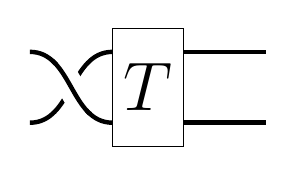
\begin{tikzpicture}[baseline=-0.65ex, scale=0.15]
        \begin{knot}[clip width=6, end tolerance=1pt, flip crossing/.list={1}]
            \strand[ultra thick] (-10, -3) [in=180, out=0] to (-3, 3);
            \strand[ultra thick] (-10, 3) [in=180, out=0] to (-3, -3);
            \draw (-3, -5) rectangle (3, 5);
            \node at (0, 0) {\Huge {$T$}};
            \draw[ultra thick] (3, -3) to (10, -3);
            \draw[ultra thick] (3, 3) to (10, 3);
        \end{knot}
    \end{tikzpicture}
    \quad $\stackrel{\mathrm{flype}}{\cong}$ \quad
    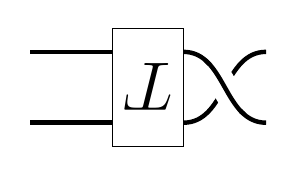
\begin{tikzpicture}[baseline=-0.65ex, scale=0.15]
        \begin{knot}[clip width=6, end tolerance=1pt]
            \strand[ultra thick] (10, -3) [in=0, out=180] to (3, 3);
            \strand[ultra thick] (10, 3) [in=0, out=180] to (3, -3);
            \draw (-3, -5) rectangle (3, 5);
            \node at (0, 0) {\rotatebox[origin=c]{-180}{\Huge $T$}};
            \draw[ultra thick] (-3, -3) to (-10, -3);
            \draw[ultra thick] (-3, 3) to (-10, 3);
        \end{knot}
    \end{tikzpicture}
    \caption{Ruch flype}%
\end{figure}

Całkiem inną taktykę szukania węzłów przyjał wielebny Thomas Kirkman: zaczynał od małego zbioru "nieredukowalnych" rzutów, do których systematycznie dokładał skrzyżowania.
\index[persons]{Kirkman, Thomas}%
Od początku był zainteresowany głównie alternującymi węzłami; w~1885 roku wydrukował diagramy 634 węzłów o~dziesięciu skrzyżowaniach.
% wielebny => Adams, s. 31

\begin{definition}[węzła, Kirkmana, w stu słowach]
    \emph{By a Knot of $n$ crossings, I understand a~reticulation of any number of meshes of two or more edges, whose summits, all tessaraces, are each a~single crossing, as when you cross your forefingers straight or slightly curved, so as not to link them, and such meshes that every thread is either seen, when the projection of the Knot with its $n$ crossings and no more is drawn in double lines, or conceived by the reader of its course when drawn in single line, to pass alternately under and over the threads to which it comes at successive crossings.}
\end{definition}

Wiemy, że Tait czytał czasopismo zawierające diagramy Kirkmana i~wykorzystał je do opracowania prawie kompletnej listy węzłów alternujących o~mniej niż 11 skrzyżowaniach.
Tuż przed oddaniem jej do druku odkrył inny spis węzłów stworzony przez amerykańskiego naukowca Charlesa Little'a.
\index[persons]{Little, Charles}%
Znalazł wtedy jeden duplikat u~siebie, natomiast u Little'a jeden duplikat i~jedno pominięcie.


\input{10-introduction/102b-history-10}


\subsubsection{Jedenaście skrzyżowań}
Na dalszy postęp musieliśmy czekać do lat sześćdziesiątych.
Wtedy to John Conway \cite{conway1970} znalazł prawie wszystkie pierwsze węzły o~mniej niż 12 skrzyżowaniach oraz sploty o~mniej niż 11 skrzyżowaniach.
\index[persons]{Conway, John}%
Odkrył jeden duplikat oraz jedenaście pominięć w~starych tablicach Little'a (do 11 skrzyżowań), ale sam zgubił cztery węzły.
Naprawienie błędu zajęło chwilę: dwa brakujące węzły zawierała praca magisterska Lombardero z~1968 roku, dwa odkrył Caudron około 1980 roku \cite{caudron1982}.
\index[persons]{Caudron, Alain}%
\index[persons]{Lombardero, David}%
Conway też popełnił dwa duplikaty: współcześnie bardziej znany to para Perko, węzeł reprezentowany przez dwa diagramy aż do tablic Rolfsena.
\index{para Perko}%
Nazywamy ją tak, ponieważ została dostrzeżona przez Perko \cite{perko1974}, który bezskutecznie próbował odróżnić składniki pary diedralnym indeksem zaczepienia: dla obydwu diagramów wynosi on $32/11$.
\index[persons]{Perko, Kenneth}%
% https://www.researchgate.net/profile/Ken-Perko/publication/299560799_The_History_of_the_Perko_Pair/links/56ff0ba508aea6b77468d550/The-History-of-the-Perko-Pair.pdf both knots yielded a 5-fold dihedral linking number of 32/11
Jako przyczynę tak długiego niezauważenia pary Perko podaje się hipotezę Little'a, że spin minimalnego diagramu jest niezmiennikiem, gdyż błędnie założył, że 2-przejścia oraz flype wystarczają do zmiany dowolnego minimalnego diagramu w~inny.
% DICTIONARY;2-pass move;2-przejście;-
\index{spin}%
\index{2-przejście}%
\index{flype}%
\index[persons]{Little, Charles}% 
(Diagramy pary Perko mają różny spin).
Zachęcamy w~tym miejscu do nieprzeskakiwania strony \pageref{rolfsens_mistake}, gdzie para Perko pojawia się raz jeszcze.
Mniej znany duplikat wystąpił w~tablicy splotów do 10 skrzyżowań, gdzie \texttt{2.-2.-20.20} jest lustrem \texttt{8*-20:-20}.

Pomimo opisanych wyżej drobnych niepowodzeń, metodę Conwaya (mającą fundamenty w~pomysłach Kirkmana) uznaje się za bardzo dobrą.
Conway potrzebował zaledwie kilku godzin na przeprowadzenie swojej klasyfikacji; a my używamy jej po dziś dzień, na przykład Tuzun, Sikora zweryfikowali dzięki niej hipotezę \ref{con:jones} do 24 skrzyżowań.
\index[persons]{Tuzun, Robert}%
\index[persons]{Sikora, Adam}%

Rękopis \cite{siebenmann1979} (albo \cite{bonahon1989}?) Bonahona, Siebenmanna klasyfikuje węzły algebraiczne.
\index[persons]{Bonahon, Francis}%
\index[persons]{Siebenmann, Laurent}%
Kres ery ręcznych obliczeń nastąpił, gdy z~nielicznymi niealgebraicznymi węzłami do 11 skrzyżowań poradził sobie Perko \cite{perko1980}, \cite{perko1982}.
\index[persons]{Perko, Kenneth}%

\begin{remark}[John Horton Conway]
    Matematyk brytyjski urodzon w 1937 roku w Liverpoolu, zmarł w 2020 roku w New Brunswick, New Jersey.
    Był wszechstronnie uzdolniony: opracował grę w~życie (jeden z pierwszych i najbardziej znanych przykładów automatów komórkowych) oraz kropki (razem z Patersonem, polega na łączeniu kropek liniami tak, by się nie przecinały -- po angielsku \emph{sprouts}); ustalił, że poza sześcioma regularnymi 4-wielotopami oraz dwoma nieskończonymi seriami zaczynającymi się od dwugraniastosłupa i antydwugraniastosłupa istnieją 64 wypukłe jednorodne 4-wielotopy; znalazł grupę automorfizmów kraty Leecha, pokazał, że każą liczbę naturalną można zapisać jako 37 piątych potęg oraz wskazał przykład funkcji, która jest nigdzie ciągła i ma wszędzie własność Darboux.
    Dla nas najciekawsza jest jego praca \cite{conway1970} o supłach.
\end{remark}

% MAKOTO SAKUMA - A SURVEY OF THE IMPACT OF THURSTON’S WORK ON KNOT THEORY
% through hand calculation of homological invariants (in particular linking invariants) of finite branched coverings for those knots that are not covered by Bonahon and Siebenmann’s result described in Subsection 4.1. See [268] for an interesting historical note.



\input{10-introduction/102b-history-13}


\subsubsection{Szesnaście skrzyżowań}
Około roku 1998 Hoste z~Weeksem oraz niezależnie Thistlethwaite \cite{thistlethwaite1998} znaleźli 1 701 936 pierwszych węzłów do 16 skrzyżowań.
\index[persons]{Hoste, Jim}%
\index[persons]{Thistlethwaite, Morwen}%
\index[persons]{Weeks, Jeff}%
Używali przy tym różnych podejść: Hoste z Weeksem wykorzystywali niezmienniki hiperboliczne oraz program SnapPea; Thistlethwaite natomiast wzbogacił zestaw ruchów Reidemeistera o flype, przejście, 2-przejście, ruch Perko oraz kilka innych ezoterycznych przekształceńtak, żeby poradzić sobie z upartymi parami diagramów.
Wśród pierwszych węzłów do 16 skrzyżowań na 32 wyjątkowe (niehiperboliczne) węzły składa się 12 węzłów torusowych oraz 20 satelitów trójlistnika.
To samo jeszcze raz napiszemy na stronie \pageref{page:nonhyperbolic_below_16}.




\subsubsection{Dziewiętnaście skrzyżowań}
Artykuł \cite{thistlethwaite98} zawiera informację, że jego autorzy szukają węzłów o~17 skrzyżowaniach, ale my nie doszukaliśmy się żadnej późniejszej publikacji na ten temat.
\index[persons]{Hoste, Jim}%
\index[persons]{Thistlethwaite, Morwen}%
\index[persons]{Weeks, Jeff}%
W 2004 Flint, Rankin oraz Schermann \cite{rankin04} znaleźli alternujące węzły do 22 skrzyżowań (obliczenia na stacji roboczej z procesorem Xeon oraz 3 gigabajtami pamięci zajęły około 45 godzin), po czym długo nie działo się nic.
\index[persons]{Flint, Ortho}%
\index[persons]{Rankin, Stuart}%
\index[persons]{Schermann, John}%

Dopiero w 2020 Burton \cite{burton20} stablicował węzły pierwsze do 19 skrzyżowań: \emph{,,Here we extend the tables from 16 to 19 crossings, with a total of 352 152 252 distinct non-trivial prime knots.''}
\index[persons]{Burton, Benjamin}%

Thistlethwaite opublikował na swojej stronie internetowej, że znalazł węzły pierwsze do 20 skrzyżowań; czekamy na publikację w renomowanym czasopiśmie.
Jeżeli nie popełnił żadnego błędu, to mamy 199 631 989 alternujących i 1 647 687 439 niealternujących węzłów pierwszych o~dwudziestu skrzyżowaniach.
\index[persons]{Thistlethwaite, Morwen}%
% https://web.math.utk.edu/~morwen/k20v4.pdf



\subsubsection{Sploty}
Cerf \cite{cerf98} pisze, że Conway \cite{conway70} znalazł wcześniej sploty do 10 skrzyżowań, zaś Caudron \cite{caudron82} poprawił wynik do 11 skrzyżowań, ale wszystkie te sploty są niezorientowane, a~naukowcy potrzebują zorientowanych.
\index[persons]{Cerf, Corinne}%
\index[persons]{Conway, John}%
\index[persons]{Caudron, Alain}%
Problem został zaadresowany najpierw przez Dolla i Hoste'a \cite{doll91}, którzy wydali na mikrofilmie tablicę splotów zorientowanych do 9 skrzyżowań, ale ich diagramy nie zawsze pasowały do tych narysowanych w~książce Rolfsena.
\index[persons]{Doll, Helmut}%
\index[persons]{Hoste, Jim}%

Cerf obiecuje pogodzić punkty widzenia Rolfsena oraz Dolla/Hoste'a i tworzy własną tablicę zorientowanych splotów do 11 skrzyżowań.
Sprawdziła jednocześnie poprawność starszych tablic Conwaya -- i nie znalazła tam żadnych błędów.

% https://sci-hub.se/https://doi.org/10.1016/B978-044451452-3/50006-X
Wiemy od Hostego, że Jablan \cite{jablan99} znalazł alternujące sploty o 12 skrzyżowaniach w duchu metod Kirkmana i Conwaya.
\index[persons]{Jablan, Slavik}%
Praca Jablana została wydrukowana w 1999 roku.
W 2001 roku Thistlethwaite posiadał tablicę pierwszych splotów alternujących do 19 skrzyżowań, jednak wygląda na to, że nigdy jej nie opublikował.
% 2001 wiem to z M. Thistlethwaite, Prime unoriented alternating links to 19 crossings, unpublished table (2001)., które wiem z Mathematical Constants II - Strona 631
\index[persons]{Thistlethwaite, Morwen}%
W 2007 roku Fontaine, Rankin, Flint znaleźli liczbę pierwszych splotów alternujących o 20, 21, ..., 24 skrzyżowaniach.
% 2007 wiem to z https://oeis.org/A049344
\index[persons]{Fontaine, Bruce}%
\index[persons]{Rankin, Stuart}%
\index[persons]{Flint, Ortho}%

Klasyfikację splotów o 12 i 13 skrzyżowaniach znaleźliśmy w pracy magisterskiej Dylana Faullina (jego zdaniem jest ich, odpowiednio, 6447 i 28239).
\index[persons]{Faullin, Dylan}%
Z niezrozumiałych dla nas przyczyn pomimo upływu prawie dwóch dekad, ten wynik pozostaje raczej nieznany.
Nie ma go na przykład w ciągu \href{https://oeis.org/A086771}{A086771} w bazie danych OEIS.




\section{Hipotezy Taita}
\index{hipoteza!Taita|(}%

Tait na podstawie węzłów o małej liczbie skrzyżowań  wysunął około 1898 roku trzy lub cztery hipotezy.
Nie jest jasne, czy chodziło mu o wszystkie węzły, czy tylko te alternujące.
Uchylamy tutaj rąbka tajemnicy i~podajemy treść hipotez już teraz; dowód ze szczegółami odkładając na później, aż do sekcji \ref{sub:tait_conjectures}.
Tam też wspomnimy krótko o technikach użytych w dowodach pozostałych trzech.

\begin{conjecture}[I hipoteza Taita]
\index{indeks skrzyżowaniowy}%
\label{con:tait_1}%
    Zredukowany alternujący diagram splotu ma minimalny indeks skrzyżowaniowy.
\end{conjecture}

Najpierw znaleziono dowód korzystający z wielomianu Jonesa: dokonali tego w 1987 roku równocześnie Kauffman \cite{kauffman1987}, Murasugi \cite{murasugi1987} oraz Thistlethwaite \cite{thistlethwaite1987}.
\index[persons]{Kauffman, Louis}%
\index[persons]{Murasugi, Kunio}%
\index[persons]{Thistlethwaite, Morwen}%
Trzydzieści lat później Greene \cite{greene2017} zaprezentował geometryczne podejście do problemu.
\index[persons]{Greene, Joshua}%

\begin{conjecture}[II hipoteza Taita]
\index{spin}%
    Dwa zredukowane diagramy alternujące jednego węzła mają ten sam spin.
\end{conjecture}

Pierwsze dowody pochodzą znowu od Kauffmana \cite{kauffman1987} oraz Thistlethwaite'a \cite{thistlethwaite1987}.
\index[persons]{Kauffman, Louis}%
\index[persons]{Thistlethwaite, Morwen}%
Dla niektórych II hipoteza brzmi inaczej (,,achiralny splot alternujący ma zerowy spin''), dla innych jest prostym wnioskiem z naszego sformułowania.

\begin{conjecture}[III hipoteza Taita]
\index{flype}%
    Niech $D_1, D_2$ będą zredukowanymi alternującymi diagramami zorientowanego pierwszego splotu.
    Wtedy diagram $D_2$ można otrzymać z~$D_1$ korzystając jedynie z~ruchu \emph{flype}.
\end{conjecture}

Trzecią hipotezę udowodnił Menasco wspólnie z~Thistlethwaitem \cite{menasco1993}.
\index[persons]{Menasco, William}%
\index[persons]{Thistlethwaite, Morwen}%
Wynika z~niej, że dwa zredukowane diagramy alternujące tego samego węzła mają ten sam spin.
Nie jest prawdziwa dla niealternujących splotów, przez co w~tablicach węzłów tak długo mieliśmy duplikat -- parę Perko.
\index{para Perko}%

Czasami mówi się jeszcze o IV hipotezie: że zwierciadlane węzły mają parzysty indeks skrzyżowań.
\index{węzeł!zwierciadlany}
Ta okazała się fałszywa.

\index{hipoteza!Taita|)}%

% koniec podsekcji Hipotezy Taita



\input{10-introduction/102f-codes}


\input{10-introduction/103-operations}
\input{10-introduction/104-primality}
\input{10-introduction/105-numerical_invariants}

\chapter{Niezmienniki kolorowe}
\input{20-colours/200-intro}
\input{20-colours/201-matrix}
\input{20-colours/202-group}

\section{Kwandle i wraki}
\index{kwandel|(}%

Sekcja ta powstała częściowo w~oparciu o~notatki autorstwa Bergera, Geriga\footnote{dostępne pod adresem \url{https://scholar.harvard.edu/files/gerig/files/knotnotes.pdf}} oraz Bergera, Flannery'ego i~Sumnichta\footnote{dostępne pod adresem \url{https://github.com/thyrgle/191_Final_Project/blob/master/paper.pdf}}; ale najlepiej zacząć od długiej na trzy strony odpowiedzi Nelsona \cite{nelson2016} na pytanie ,,czym jest kwandel?''.
\index[persons]{Berger, Andrew}%
\index[persons]{Gerig, Chris}%
\index[persons]{Flannery, Brandon}%
\index[persons]{Sumnicht, Christopher}%
\index[persons]{Nelson, Sam}%
Należy przy tym pamiętać, że jest to dość niszowe zagadnienie, na przykład Burde, Zieschang, Heusener \cite[s. 11]{burde2014} poświęcają mu pięć wierszy i~odsyłają Czytelnika do pracy Fenna, Rourkego \cite{fenn1992}.
\index[persons]{Fenn, Roger}%
\index[persons]{Rourke, Colin}%
Dużo otwartych problemów dotyczących kwandli można znaleźć u~Ohtsukiego \cite[s. 455-465]{ohtsuki2002}.

Kwandle pierwszy raz odkryli Conway z Wraithem około 1959 roku, jeszcze jako studenci I stopnia na uniwersytecie w Cambridge, w nieopublikowanej korespondencji między sobą (patrz definicja przed definicją \ref{def:quandle}).
\index[persons]{Conway, John}%
\index[persons]{Wraith, Gaven}%
Ponownie uczyniono to latach 80. XX wieku: Joyce w~1982 jako kwandle, Matwiejow w tym samym roku pod nazwą grupoidy rozdzielne, wreszcie Brieskorn w 1986 jako zbiory automorficzne.
\index[persons]{Joyce, David}%
\index[persons]{Matwiejow, Siergiej (Матвеев, Сергей Владимирович)}%
\index[persons]{Brieskorn, Egbert}%
\index{grupoid rozdzielny|see {kwandel}}%
\index{zbiór automorficzny|see {kwandel}}%
Joyce zapytany o znaczenie słowa \emph{quandle} odparł \emph{,,I needed a usable word. Distributive algebra had too many syllables. Piffle was already taken. I tried trindle and quagle, but they didn’t seem right, so I went with quandle''}.\footnote{Źródło: blog Johna Baeza \url{https://golem.ph.utexas.edu/category/2015/05/the_origin_of_the_word_quandle.html}}
\index[persons]{Joyce, David}%

Conway nazwał wraki wrakami (\emph{wracks}), by częściowo zażartować z~nazwiska jego kolegi Wraitha, a częściowo by zaznaczyć, że są one tym, co zostaje z~grupy, w~której zapomniano o~mnożeniu, ale nie sprzęganiu (w~języku angielskim co najmniej od XVI wieku funkcjonuje zwrot ,,wrack and ruin'' oznaczający zniszczenie).
\index[persons]{Conway, John}%
\index[persons]{Wraith, Gaven}%
Obecnie dominuje określenie \emph{racks}.

\subsection{Kwandle}
Aksjomaty grupy stanowią uogólnienie symetrii, ponieważ składanie symetrii jest łączne, identyczność jest symetrią, funkcja odwrotna do symetrii jest symetrią.
Znajdziemy teraz słabo znaną strukturę algebraiczną, która odzwierciedla ruchy Reidemeistera (oraz aksjomatyzuje własności sprzężeń w grupach, choć jest to dla nas mniej interesujące).
\index{ruch!Reidemeistera}%

Niech $X$ będzie skończonym zbiorem kolorów wyposażonym w~działanie $\triangleright \colon X \times X \to X$.
Będziemy rysować diagramy węzłów tak, że każdemu łukowi przypisany będzie pewien kolor $x \in X$ zgodnie z następującą regułą (patrz rysunek): kiedy łuk o kolorze $x$ przechodzi pod biegnącym w prawo łukiem koloru $y$, staje się łukiem w kolorze $x \triangleright y$.

\begin{comment}
\[
    \LargeMinusCrossingQuandle
\]
\end{comment}

Formalnie:

% DICTIONARY;quandle;kwandel;-
\begin{definition}[kwandel]
\label{def:quandle}%
\index{kwandel}%
    Zbiór $X$ wyposażony w dwuargumentowe działanie $\triangleright$, które dla wszystkich elementów $x, y, z \in X$ spełnia trzy warunki:
    \begin{enumerate}
        \item $x \triangleright x = x$,
        \item odwzorowanie $\beta_y \colon X \to X$ dane wzorem $\beta_y(x) = x \triangleright y$ jest odwracalne,
        \item $(x \triangleright y) \triangleright z = (x \triangleright z) \triangleright (y \triangleright z)$,
    \end{enumerate}
    nazywamy kwandlem.
\end{definition}

Drugi aksjomat nazywa się czasem odwracalnością z prawej strony: znając $x \triangleright y$ oraz $y$ możemy odtworzyć element $x$, jednak znając $x$ być może nie jesteśmy w stanie odtworzyć elementu $y$.
Jedyny element $x$ taki, że $x \triangleright y = z$ nazwijmy $y \triangleleft z$.
To pozwala podać trochę inną definicję kwandli, którą przytaczamy jako ciekawostkę.

\begin{definition}
    Zbiór $X$ z dwuargumentowymi działaniami $\triangleright, \triangleleft$ taki, że dla wszystkich $x, y, z \in X$ zachodzi:
    \begin{align}
    x \triangleleft x & = x \\
    x \triangleright x & = x \\
    (x \triangleleft y) \triangleright x & = y \\
    x \triangleleft (y \triangleright x) & = y \\
     (x \triangleright z) \triangleright (y \triangleright z) & = (x \triangleright y) \triangleright z \\
    (x \triangleleft y) \triangleleft (x \triangleleft z) & = x \triangleleft (y \triangleleft z)
    \end{align}
    nazywamy kwandlem.
\end{definition}

Pokażemy teraz, czemu aksjomaty kwandli można traktować jako przetłumaczenie ruchów Reidemeistera na język algebry.
\index{ruch!Reidemeistera}%

\begin{proposition}[niezmiennik zliczający]
\index{niezmiennik!zliczający}%
    Niech $X$ będzie skończonym kwandlem.
    Liczba etykietowań diagramu elementami kwandla $X$ jest niezmiennikiem węzłów, zwanym niezmiennikiem zliczającym.
\end{proposition}
    
\begin{proof}
    Musimy pokazać, że etykiety na diagramiem przed każdym ruchem Reidemeistera wyznaczają jednoznacznie układ etykiet po tym ruchu.
    Pierwszy i drugi ruch:
\begin{comment}
    \begin{figure}[H]
        \begin{minipage}[b]{.48\linewidth}
        \[
            \LargeReidemeisterOneRightQuandleProof
            \stackrel{R_1}{\cong}
            \LargeReidemeisterOneStraightQuandleProof
        \]
        \end{minipage}
        \begin{minipage}[b]{.48\linewidth}
        \[
            \LargeReidemeisterTwoQuandleA \cong \LargeReidemeisterTwoQuandleB
        \]
        \end{minipage}
    \end{figure}
\end{comment}
    Trzeci ruch:
\begin{comment}
    \[
        \LargeReidemeisterThreeQuandleA \cong \LargeReidemeisterThreeQuandleB \qedhere
    \]
\end{comment}
\end{proof}

Wiele znanych struktur algebraicznych okazuje się być źródłem kwandli:

\begin{example}[kwandel cykliczny/diedralny]
\index{kwandel!cykliczny}%
\index{kwandel!diedralny}%
    Grupa abelowa z działaniem $x \triangleright y = 2y - x$.
\end{example}

\begin{example}[kwandle sprzężone]
\index{kwandel!sprzężony}%
    Grupa z działaniem $x \triangleright y = y^{-n} x y^n$ dla każdego $n \in \N$.
\end{example}

\begin{example}[kwandel Alexandera]
\index{kwandel!Alexandera}%
    Moduł nad pierścieniem $\Z[t, 1/t]$ wielomianów Laurenta z~działaniem $x \triangleright y = tx + (1-t) y$.
\end{example}

Dionísio, Lopes \cite[s. 1043]{lopes2003} potrzebują skończonych kwandli Alexandera, mają postać $(\Z/n\Z)[t, 1/t] / h(t)$, gdzie $h$ jest pewnym unormowanym wielomianem.

\begin{example}[kwandel symplektyczny]
\index{kwandel!symplektyczny}%
    Przestrzeń liniowa i antysymetryczna forma dwuliniowa $\langle \bullet | \bullet \rangle$ z działaniem $x \triangleright y = x + \langle x | y \rangle \cdot y$.
\end{example}

Żeby opowiedzieć, jak wyglądały poszukiwania małych kwandli, musimy wprowadzić dwie definicje.

\begin{definition}[homomorfizm kwandli]
    Niech $Q_1, Q_2$ będą kwandlami.
    Funkcję $f \colon Q_1 \to Q_2$ spełniającą warunek
    \begin{equation}
        \forall x, y \in Q_1 : f(x \triangleright y) = f(x) \triangleright f(y),
    \end{equation}
    nazywamy homomorfizmem kwandli.
\end{definition}

\begin{definition}[kwandel spójny]
\index{kwandel!spójny}%
    Niech $Q$ będzie kwandlem.
    W grupie wszystkich automorfizmów $Q$ można wyróżnić grupę generowaną przez automorfizmy wewnętrzne $\beta_y(x) = x \triangleright y$.
    Jeżeli działanie tej podgrupy na $Q$ jest przechodnie, kwandel $Q$ nazywamy spójnym.
\end{definition}

Dionísio, Lopes \cite{lopes2003} znaleźli 10 kwandli Alexandera, które odróżniają prawie każde dwa spośród 249 węzłów pierwszych do 10 skrzyżowań; rozstrzygnięcia brak dla 962 z 30876 par.
\index[persons]{Dionísio, Miguel}%
\index[persons]{Lopes, Pedro}%
Po upływie prawie dekady Vendramin \cite{vendramin2012} wytropił wszystkie 431 kwandli spójnych rzędu 35 lub mniejszego.
\index[persons]{Vendramin, Leandro}%
Clark, Elhamdadi, Saito oraz Yeatman \cite{clark2013} pokazali niedawno zbiór 26 kwandli, które razem odróżniają od siebie wszystkie 2977 zorientowanych węzłów pierwszych o~co najwyżej 12 skrzyżowaniach.
\index[persons]{Clark, William}%
\index[persons]{Elhamdadi, Mohamed}%
\index[persons]{Saito, Masahico}%
\index[persons]{Yeatman, Timothy}%
Największy z~nich jest rzędu 182.

Joyce w swojej rozprawie doktorskiej przypisał każdemu węzłowi $K$ pewien szczególny kwandel $Q(K)$, kwandel podstawowy.
\index[persons]{Joyce, David}%
\index{kwandel!podstawowy}%
Jest to niezmiennik generowany przez łuki diagramu związany relacjami pochodzącymi ze skrzyżowań, tak jak w~definicji grupy węzła.
Wprawdzie znajomość kwandla $Q(K)$ pozwala odtworzyć węzęł $K$ z dokładnością do jego orientacji, ale jak nietrudno się domyślić, ceną za to jest trudność w~jego wyznaczaniu.

Na przykład Niebrzydowski, Przytycki \cite{niebrzydowski2009} pokazali, że
\index[persons]{Niebrzydowski, Maciej}%
\index[persons]{Przytycki, Józef}%

\begin{example}
    Kwandel podstawowy trójlistnika  jest izomorficzny z~pewnym rzutowym pierwotnym podkwandlem\footnote{Cokolwiek to znaczy!} odwzorowań liniowych przestrzeni symplektycznej $\Z \oplus \Z$
\end{example}

Słabszym, choć prostszym w znalezieniu niezmiennikiem jest liczba homomorfizmów z kwandla danego węzła w pewien wybrany wcześniej kwandel $Q$.
% wiem to z nLab

\subsection{Półki, wraki i wrzeciona}
Aksjomaty grupy można wzmacniać (grupy abelowe) lub osłabiać (monoidy).
Podobnie czyni się z aksjomatami kwandli.
Kwandle inwolutywne odpowiadają węzłom bez orientacji, wraki dobrze opisują węzły obramowane, i tak dalej.
\index{węzeł!niezorientowany}%
% TODO: w zorientowanym dać patrz też do niezorientowanego?
\index{węzeł!obramowany}%

\begin{definition}[kwandel inwolutywny]
\index{kwandel!inwolutywny}%
\index{kei|see {kwandel inwolutywny}}%
    Kwandel $Q$, w którym dla wszystkich $x, y \in Q$ zachodzi $x \triangleleft (x \triangleleft y) = y$, nazywamy inwolutywnym albo kei.
\end{definition}

Kwandle inwolutywne badał jako pierwszy Mituhisa Takasaki (1943).
\index[persons]{Takasaki, Mituhisa}%
Szukał niełącznej struktury, która dobrze opisywałaby odbicia w skończonej geometrii.

% DICTIONARY;shelf;półka;-
\begin{definition}[półka]
\index{półka}%
    Zbiór $X$ wyposażony w dwuargumentowe działanie $\triangleright$ taki, że dla wszystkich elementów $x, y, z \in X$ zachodzi $(x \triangleright y) \triangleright z = (x \triangleright z) \triangleright (y \triangleright z)$, nazywamy półką.
\end{definition}

\begin{example}
\index{warkocz}%
    Niech $B_\infty$ oznacza kogranicę łańcucha $B_0 \to B_1 \to B_2 \to \ldots$, gdzie inkluzja $B_{n} \to B_{n+1}$ zadana jest przez dołączenie niesplątanego z resztą diagramu pasma, zaś $\phi$ będzie jej endomorfizmem posyłającym generator $\sigma_k$ na $\sigma_{k+1}$.
    Zbiór $B_\infty$ z działaniem $a \triangleleft b = a\phi(b)\sigma_1 \phi{a} ^{-1}$ jest półką.\footnote{Źródło: encyklopedia nLab \url{https://ncatlab.org/nlab/show/shelf}. Uwaga: symbole $\triangleleft, \triangleright$ są tam zamienione znaczeniami!}
\end{example}

To nieprzetłumaczalna gra słów: dwie półki (\emph{shelves}), lewa i prawa, które dobrze do siebie pasują, dają stojak (\emph{rack}, czyli dla nas wrak).
Jak napisała Crans \cite[s. 86]{crans2004}: \emph{,,Just as a rack is comprised of two shelves which fit together nicely, a quandle is made up of two spindles''}.
\index[persons]{Crans, Alissa}%

Półka stanowi uogólnienie dwóch obiektów -- wrzecion i~wraków.

% DICTIONARY;spindle;wrzeciono
\begin{definition}[wrzeciono]
\index{wrzeciono}%
    Zbiór $X$ z dwuargumentowym działaniem $\triangleright$ taki, że dla wszystkich elementów $x, y, z \in X$ zachodzi:
    \begin{enumerate}
        \item $x \triangleright x = x$,
        \item $(x \triangleright y) \triangleright z = (x \triangleright z) \triangleright (y \triangleright z)$
    \end{enumerate}
    nazywamy wrzecionem.
\end{definition}

% DICTIONARY;wrack;wrak
\begin{definition}[wrak]
\index{wrak}%
    Zbiór $X$ z dwuargumentowym działaniem $\triangleright$ takim, że dla każdej trójki elementów $x, y, z \in X$ zachodzi:
    \begin{enumerate}
        \item odwzorowanie $\beta_y \colon X \to X$ dane wzorem $\beta_y(x) = x \triangleright y$ jest odwracalne,
        \item $(x \triangleright y) \triangleright z = (x \triangleright z) \triangleright (y \triangleright z)$
    \end{enumerate}
    nazywamy wrakiem.
\end{definition}

\begin{example}
    % https://www1.cmc.edu/pages/faculty/VNelson/quandles.html
    Zbiór $X = \{1, 2, \ldots, n\}$ i permutacja $\sigma \in S_n$ z działaniem $x \triangleright y = \sigma(x)$.
\end{example}

\begin{example}
    % https://www1.cmc.edu/pages/faculty/VNelson/quandles.html
    Moduł nad pierścieniem $\Z[t^{\pm 1}, s]/(s^2 - (1-t)s)$ z działaniem $x \triangleright y = tx+sy$.
\end{example}

\index{węzeł!obramowany}% framed?
Wraki są naturalnym niezmiennikiem węzłów obramowanych, bo dobrze współgrają z II, III oraz podwójnym I ruchem Reidemeistera, który to nie zmienia spinu diagramu:
\begin{comment}
\[
    \LargeReidemeisterOneLeftRightQuandleProof
    \cong
    \LargeReidemeisterOneStraightQuandleProofRotated
\]
\end{comment}

\index{kwandel|)}

% Koniec sekcji Kwandle i wraki



\chapter{Niezmienniki wielomianowe}

Wszystkie poznane dotąd niezmienniki (poza długością sznurową) przyjmowały całkowite wartości.
Teraz poszerzymy skrzynkę z~narzędziami o~klasyczne wielomiany Alexandera, Jonesa, HOMFLY; ale też późniejsze: BLM/Ho, Kauffmana oraz niezmienniki skończonego typu.
Co ciekawe, wielomiany te wywodzą się z~różnych działów matematyki: wielomian $\alexander$ Alexandera z~homologii pewnej przestrzeni nakrywającej, $\jones$ Jonesa: z~algebr von Neumanna.
HOMFLY (albo raczej HOMFLY-PT) to ich naturalne uogólnienie.

Atrakcyjnym wprowadzeniem była przygotowana przez matematyków niemieckich (przez to dostępna tylko w~ich języku) praca \cite{gellert2009}.
Pierwotnymi artykułami były \cite{alexander1928}, \cite{jones1985} oraz \cite{homfly1985}, wszystkie należą do przełomowych w~kombinatorycznej teorii węzłów.


\input{30-polynomials/301-alexander}

\section{Wielomian Jonesa}
\index{wielomian!Jonesa|(}%
Drugi wielomianowy niezmiennik, jaki poznamy, spełnia bardzo podobną relację kłębiastą (porównaj: \ref{eqn:alexander_skein} versus \ref{eqn:jones_skein}), co ten z poprzedniej sekcji.
Zaczniemy od bardzo ogólnikowego opisu algebry Temperleya-Lieba i śladu Markowa; dwóch składników w~konstrukcji Jonesa.
Szczegółowo zajmiemy się późniejszym odkryciem Kauffmana, bo wykorzystał lubiane przez nas diagramy i~ruchy Reidemeistera.
Opiszemy krótko, jak zmienia się wielomian podczas odbijania, odwracania i dodawania.
Na koniec podamy dowód I hipotezy Taita, wspomnimy też, jaką rolę wielomian Jonesa odegrał w dowodzie pozostałych dwóch hipotez.

\input{30-polynomials/302b-temperley}

\input{30-polynomials/302a-kauffman}


\subsection{Odróżnianie węzłów i splotów wielomianem Jonesa}
Wielomian Jonesa często (chociaż nie zawsze) odróżnia od siebie sploty lepiej niż wielomian Alexandera.
Na przykład: wielomian Alexandera wszystkich splotów rozszczepialnych jest taki sam (stwierdzenie \ref{prp:alexander_unlinks}), więc nie odróżnia wcale niesplotów.
Dla porównania, wielomian Jonesa odróżnia je wszystkie:

\begin{proposition}
\label{prp:jones_trivial_link}%
    Wielomianem Jonesa splotu trywialnego o $n$ ogniwach jest
    \begin{equation}
        \jones(K_n) = \left(-\sqrt{t} - \frac{1}{\sqrt {t}}\right)^{n-1}.
    \end{equation}
\end{proposition}

Co więcej, wielomian Jonesa odróżnia od siebie dowolne dwa węzły pierwsze o~co najwyżej 9 skrzyżowaniach.
Dalej występują już kolizje, oto pełna ich lista do 10 skrzyżowań:

\renewcommand*{\arraystretch}{1.4}
\footnotesize
\begin{longtable}{lcccccccccccccc}
    $K_1$ & \rotatebox{90}{$5_{1}$} & \rotatebox{90}{$8_{8}$} & \rotatebox{90}{$8_{16}$} & \rotatebox{90}{$10_{22}$} & \rotatebox{90}{$10_{25}$} & \rotatebox{90}{$10_{40}$}  & \rotatebox{90}{$10_{41}$}  & \rotatebox{90}{$10_{43}$} & \rotatebox{90}{$10_{59}$} & \rotatebox{90}{$10_{60}$} & \rotatebox{90}{$10_{71}$}  & \rotatebox{90}{$10_{73}$}  & \rotatebox{90}{$10_{81}$} & \rotatebox{90}{$10_{137}$} \\
    $K_2$ & \rotatebox{90}{$10_{132}$} & \rotatebox{90}{$10_{129}$} & \rotatebox{90}{$10_{156}$} & \rotatebox{90}{$10_{35}$} & 
\rotatebox{90}{$10_{56}$} & \rotatebox{90}{$10_{103}$} & \rotatebox{90}{$10_{94}$} & \rotatebox{90}{$10_{91}$} & \rotatebox{90}{$10_{106}$} & \rotatebox{90}{$10_{86}$} & \rotatebox{90}{$10_{104}$\,\,} & \rotatebox{90}{$10_{83}$} & \rotatebox{90}{$10_{109}$} & \rotatebox{90}{$10_{155}$}  \\
    \hline
\end{longtable}
% ZWERYFIKOWANO: funkcja jones_collisions
\normalsize

Jones wiedział, że wielomianowe niezmienniki nie radzą sobie z~odróżnianiem od siebie mutantów, dlatego zapytał, czy jego wielomian wykrywa niewęzły.
Pozostaje to otwartym problemem do dziś (patrz na przykład do zbioru problemów Ohtsukiego \cite[s. 381]{ohtsuki02}).

\begin{conjecture}
\index{hipoteza!o wielomianie Jonesa i niewęźle}%
\label{con:jones}%
    Niech $K$ będzie węzłem.
    Jeśli $\jones_K(t) \equiv 1$, to $K$ jest niewęzłem.
\end{conjecture}

Co przemawia za prawdziwością hipotezy?
Wiemy, że jest prawdziwa w~wielu szczególnych przypadkach: dla węzłów alternujących (wynika to z I hipotezy Taita \ref{con:tait_1}), adekwatnych (Lickorish, Thistlethwaite \cite{lickorish88}), póładekwatnych (dużo później Stojmenow \cite{stoimenow11}), dodatnich (także Stojmenow, chyba w \cite{stoimenow03}) oraz prawie alternujących: węzeł jest prawie alternujący, jeżeli nie jest alternujący, ale odwrócenie jednego skrzyżowania na pewnym diagramie sprawia, że takim się staje (Lowrance, Spyropoulos \cite{lowrance17}).
\index{splot!alternujący}%
\index{splot!adekwatny}%
\index{splot!póładekwatny}%
\index{splot!dodatni}%
\index{splot!prawie alternujący}%
\index[persons]{Thistlethwaite, Morwen}%
\index[persons]{Lickorish, William}%
\index[persons]{Stojmenow, Alexander}%
\index[persons]{Lowrance, Adam}%
\index[persons]{Spyropoulos, Dean}%
Homologia Chowanowa stanowi uogólnienie wielomianu Jonesa i wykrywa niewęzeł (patrz fakt \ref{khovanov_detects_unknot}).
\index{homologia!Chowanowa}%

Hipotezę zweryfikowano komputerowo dla węzłów o~małej liczbie skrzyżowań.
W latach dziewięćdziesiątych Hoste, Thistlethwaite, Weeks \cite{thistlethwaite98} zrobili to podczas tablicowania węzłów spełniających $\crossing K \le 16$.
\index[persons]{Hoste, Jim}%
\index[persons]{Thistlethwaite, Morwen}%
\index[persons]{Weeks, Jeff}%
Wynik poprawiano:
Dasbach, Hougardy \cite{hougardy97} w~1997 do $\crossing K \le 17$; 
\index[persons]{Dasbach, Oliver}%
\index[persons]{Hougardy, Stefan}%
Yamada \cite{yamada00} w~2000 do $\crossing K \le 18$;
\index[persons]{Yamada, Shuji}%
wreszcie Tuzun, Sikora \cite{tuzun18} w~2016 do $\crossing K \le 22$,
\index[persons]{Sikora, Adam}%
\index[persons]{Tuzun, Robert}%
potem (w \cite{tuzun21}) w~2020 do $\crossing K \le 24$.
Ośmiordzeniowe procesory Intel Xeon L5520 z Uniwersytetu w~Buffalo potrzebowały na to łącznie 41,8 lat pracy.

Co przemawia za nieprawdziwością hipotezy?
Najpierw Thistlethwaite w~\cite{thistlethwaite01} wskazał dwa sploty z~dwoma oraz jeden z~trzema ogniwami, których wielomian Jonesa nie odróżnia od niesplotów o~takiej samej liczbie ogniw.
\index[persons]{Thistlethwaite, Morwen}%
Wynik bardzo szybko bardzo poprawiono: Eliahou, Kauffman i~Thistlethwaite w~pracy \cite{eliahou03} znaleźli nieskończoną rodzinę splotów o~tej samej własości.
\index[persons]{Eliahou, Shalom}%
\index[persons]{Kauffman, Louis}%
Kauffman znalazł dużo wcześniej nietrywialny węzeł wirtualny, którego wielomian Jonesa jest trywialny.

\begin{proposition}
\index{splot!Hopfa}%
\index{węzeł!satelitarny}%
    Niech $k \ge 2$ będzie liczbą naturalną.
    Istnieje nieskończenie wiele pierwszych satelitów splotu Hopfa z $k$ ogniwami, których wielomian Jonesa nie odróżnia od niesplotu z $k$ ogniwami.
\end{proposition}



\input{30-polynomials/302e-skein}

\input{30-polynomials/302f-mirror_reverse}

\input{30-polynomials/302g-roots_of_unity}

\index{wielomian!Jonesa|)}%

\input{30-polynomials/302c-span}


\input{30-polynomials/303-homfly}
\input{30-polynomials/304-blmho}

\section{Wielomian Kauffmana}
\index{wielomian!Kauffmana|(}%
Mniej więcej w~tym samym czasie, gdy odkryto wielomian BLM/Ho, Kauffman \cite{kauffman1990} opisał sposób, jak uogólnić ten niezmiennik do odróżniającego lustra.
\index[persons]{Kauffman, Louis}%
Wielomianu $F$ Kauffmana nie należy mylić z~klamrą Kauffmana $\langle \ldots \rangle$!

\begin{definition}[wielomian Kauffmana]
    Niech $L$ będzie zorientowanym splotem, zaś $D$ ustalonym diagramem o~spinie $\writhe D$.
    Istnieje wielomian $\Lambda(L)$ wyznaczony przez relację kłębiastą (z oznaczeniami jak na stronie \pageref{unoriented_diagrams_infty})
    \begin{equation}
\begin{comment}
        \Lambda (L_+) +
        \Lambda (L_-) =
        z \cdot \left(
        \Lambda (L_0) +
        \Lambda (L_\infty)
        \right)
\end{comment}
        ,
    \end{equation}
    który jest niezmienniczy względem II i III ruchu Reidemeistera, spełnia równości:
    \begin{equation}
\begin{comment}
        \frac 1 a \Lambda \left(\MediumThinReidemeisterOneRight\right) =
        \Lambda \left(\MediumThinReidemeisterOneStraight\right)
\end{comment}
        =
\begin{comment}
        a \Lambda \left(\MediumThinReidemeisterOneLeft\right)
\end{comment}
    \end{equation}
    oraz warunek brzegowy $\Lambda(\SmallUnknot) = 1$.
    Wtedy wielomian dwóch zmiennych
    \begin{equation}
        F_L(a, z) = a^{-\writhe D} \Lambda(D),
    \end{equation}
    nazywamy wielomianem Kauffmana.
    Jest niezmiennikiem splotów.
\end{definition}

Jego związki z~wielomianem HOMFLY pozostają nieznane.
Wiemy natomiast, że

\begin{proposition}
\index{wielomian!BLM/Ho}%
    Wielomian BLM/Ho jest szczególnym przypadkiem wielomianu Kauffmana, mamy równość
    \begin{equation}
        Q(x) = F(1, x).
    \end{equation}
\end{proposition}

\begin{proposition}
\index{wielomian!Jonesa}%
    Wielomian Jonesa jest szczególnym przypadkiem wielomianu Kauffmana, mamy równość
    \begin{equation}
        \jones(t)=F(-t^{-3/4},t^{-1/4}+t^{1/4}).
    \end{equation}
\end{proposition}

Rozpatrzmy relację kłębiastą $\Lambda_+ - \Lambda_- = x(\Lambda_0 - \Lambda_\infty)$.
Prowadzi ona do wielomianu ,,z~Dubrownika'': Kauffman na pocztówce napisanej do Lickorisha z Dubrownika w~1985 roku opisał ten wielomian sądząc, że jest to nowy, niezależny od $F$ niezmiennik.
\index[persons]{Lickorish, William}%
\index{wielomian!z Dubrownika}%
\index{wielomian!Kauffmana|)}%

% Koniec sekcji Wielomian Kauffmana


\input{30-polynomials/306-vassiliev}

\chapter{Topologia algebraiczna}

Powoli kończymy definiować niezmienniki węzłów, po tym rozdziale brakować będzie tylko liczby warkoczowej.
Zaczniemy opisu grupy podstawowej dopełnienia węzła oraz prezentacji tej grupy znalezionej przez Wirtingera.
Następnie pokażemy, że każdy węzeł jest brzegiem pewnej zorientowanej powierzchni (zwanej powierzchnią Seiferta) i odkryjemy tak źródło kolejnych niezmienników: genusu, wyznacznika, sygnatury.
Nie do końca wiadomo dlaczego, ale wspomnimy krótko o~niezmienniku Arfa.
Na koniec spróbujemy przekonać czytelnika, że najciekawszą teorią homologii dla węzłów są homologie Chowanowa.

% koniec wstępu do rozdziału 4: topologia



\section{Grupa węzła}
Ponieważ dopełnienie dowolnego węzła, zarówno w przestrzeni $\R^3$ jak i $S^3$, jest łukowo spójne, jego grupa podstawowa nie zależy od wyboru punktu bazowego.
Dzięki temu poniższa definicja ma sens:

\begin{definition}[grupa węzła]
\index{grupa!węzła}%
    Niech $K$ będzie węzłem.
    Grupę podstawową jego dopełnienia,
    \begin{equation}
        \pi(L) := \pi_1 \left(\R^3 \setminus L\right),
    \end{equation}
    nazywamy grupą węzła i oznaczamy $\pi(K)$.
\end{definition}

Nie należy (i dosyć trudno jest) mylić grupy węzła z grupą kolorującą (patrz definicja \ref{def:colouring_group}).
Jak wkrótce się przekonamy, ta pierwsza jest zawsze nieskończona i poza grupą niewęzła, nieprzemienna.
Natomiast grupa kolorująca jest skończona dla splotów o~niezerowym wyznaczniku i zawsze przemienna.

Podamy najpierw kilka przykładów węzłów oraz ich grup.

\begin{example}
    Grupa niewęzła: $\Z$.
\end{example}

Z twierdzenia o pętli, czyli uogólnienia lematu Dehna wynika, że niewęzeł jest jedynym węzłem, którego grupą podstawową jest $\Z$.
% TODO: https://math.stackexchange.com/questions/3468034/knot-group-is-mathbbz-iff-k-is-the-unknot
(Pierwszy dowód lematu Dehna podał Max Dehn w 1910 roku, ale Hellmuth Kneser znalazł w 1929 lukę w dowodzie.
Z odsieczą przyszedł matematyk grecki Christos Papakyriakopoulos, który około 1957 roku nie tylko podał poprawny dowód używając jego ,,konstrukcji wieżowej'', ale uogólnił go do twierdzenia o~pętli, o~sferze).
% Wiem to z: https://en.wikipedia.org/wiki/Dehn%27s_lemma oraz Burde, Zieschang, Heusener, strona 52

\begin{example}
\label{exm:trefoil_group}%
    Grupa trójlistnika: $\langle x, y \mid x^2 = y^3\rangle$.
\end{example}

\begin{proof}
    Wynika to z (prezentacji Wirtingera i) równości
    % https://en.wikipedia.org/wiki/Tietze_transformations
    \begin{align}
        \pi_1(S^3 \setminus 3_1) & = \langle x, y, z \mid xz = yx, zy = xz, yx = zy \rangle \\
                                 & = \langle x, y \mid xyx = yxy \rangle \\
                                 & = \langle x, y, a, b \mid xyx = yxy, a = yx, b = xyx \rangle \\
                                 & = \langle x, a, b \mid xa = a^2x^{-1}, b = xa \rangle \\
                                 & = \langle a, b \mid b = a^2(ba^{-1})^{-1} \rangle \\
                                 & = \langle a, b \mid a^3 = b^2 \rangle,
    \end{align}
    prawdziwych na mocy transformacji Tietzego.
\end{proof}

Trójlistnik jest węzłem $(3, 2)$-torusowym, więc powyższy przykład stanowi szczególny przypadek grupy węzła torusowego.
Jej wyznaczenie to popularne ćwiczenie w~podręcznikach topologii algebraicznej:

\begin{example}
    Grupa węzła $(p,q)$-torusowego: $\langle x, y \mid x^p = y^q \rangle$.
\end{example}

\begin{proof}
    Wniosek z twierdzenia Seiferta-van Kampena, patrz \cite[s. 77]{kawauchi96} albo \cite[s. 47]{hatcher02}.
\end{proof}

\begin{example}
    Grupa ósemki: $\langle x, y \mid yxy^{{-1}}xy=xyx^{{-1}}yx \rangle$.
\end{example}

\begin{proposition}
    \label{prop:knot_group_invariant}
    Jeżeli węzły $L_1, L_2$ są równoważne, to grupy $\pi(L_1), \pi(L_2)$ są izomorficzne.
    Innymi słowy, grupa jest niezmiennikiem węzłów.
\end{proposition}

\begin{proof}
    Gdy dwa węzły są równoważne, istnieje izotopijny z~identycznością homeomorfizm $\R^3 \to \R^3$, który posyła pierwszy węzeł na drugi.
    Obcięty do dopełnień węzłów indukuje izomorfizm grup podstawowych.
\end{proof}

Na przykładzie grupy $\langle x,y,z \mid xyx=yxy,xzx=zxz\rangle$, która odpowiada zarówno sumie prostej różno-, jak i~jednoskrętnych trójlistników, widać że implikacja odwrotna nie zachodzi: mają one różne sygnatury (patrz uwaga za wnioskiem \ref{cor:acheiral_signature}).
Prawdziwe jest nawet ogólniejsze stwierdzenie:

\begin{proposition}
    Niech $K_1, K_2$ będą zorientowanymi węzłami.
    Wtedy węzłom $K_1 \shrap K_2$, $K_1 \shrap mr K_2$ odpowiadają izomorficzne grupy.
\end{proposition}

\begin{proof}
    Wniosek z twierdzeń o podgrupie południkowo-równoleżnikowej \cite[s. 75]{kawauchi96}.
\end{proof}

Twierdzenie odwrotne do faktu \ref{prop:knot_group_invariant} jest prawdziwe w klasie węzłów pierwszych:

\begin{proposition}
    Niech $K_1, K_2$ będą węzłami pierwszymi.
    Jeżeli ich grupy są izomorficzne, to same węzły są równoważne.
\end{proposition}

,,\emph{The group of a prime knot does not, however, necessarily determine the topological type of the exterior. Dehn hips on certain “essential” solid tori in the exteriors of torus knots and of cable knots produce Haken manifolds that are homotopically equivalent but not homeomorphic to the original exteriors and that, in fact, cannot be imbedded in $S^3$}'' (Whitten, \cite{whitten87}).
\index{rozmaitość!Hakena}%

\begin{proof}
\index[persons]{Gordon, Cameron}%
\index[persons]{Luecke, John}%
\index[persons]{Whitten, Wilbur}%
    % to jest kopia \cite[s. 76]{kawauchi96}
    Whitten pokazał w \cite{whitten87}, że węzły o~izomorficznych grupach mają homeomorficzne dopełnienia.
    Wkrótce po tym Gordon, Luecke udowodnili w~\cite{gordon89}, że nietrywialna chirurgia Dehna na nietrywialnym węźle nigdy nie daje sfery $S^3$, a~stąd wynika, że każdy homeomorfizm dopełnień węzłów można przedłużyć do homeomorfizmu $S^3$ w~siebie posyłającego jeden węzeł na drugi jako zbiory.
\index{chirurgia Dehna}%
\end{proof}

Waldhausen \cite{waldhausen68} pokazał dla pewnej dużej klasy 3-rozmaitości, że są scharakteryzowane topologicznie przez ich grupy podstawowe.
\index[persons]{Waldhausen, Friedhelm}%
Potem odkryto, że:

\begin{proposition}
    Grupa węzła wyznacza wartość jego genusu.
\end{proposition}
\begin{proof}[Niedowód]
    Jest to wniosek 3 z~pracy \cite{feustel78} Feustela.
\end{proof}
\begin{proposition}
    Grupa węzła złożonego wyznacza wartość jego liczby mostowej.
\end{proposition}
\begin{proof}[Niedowód]
    Jest to wniosek 3 z~pracy \cite{feustel78} Feustela.
\end{proof}

Wreszcie Thurston \cite{thurston82} jako efekt uboczny uzyskał kolejny wynik o grupie: hiperboliczne rozmaitości o skończonej objętości (domknięte rozmaitości lub takie, których brzeg jest zbudowany z torusów) są wyznaczone przez ich grupę podstawową.
\index[persons]{Thurston, William}%

\subsection{Grupa splotu}

Kawauchi \cite[s. 73]{kawauchi96} definiuje grupę splotu jako grupę podstawową jego dopełnienia.
Dla Milnora \cite{milnor54} grupą splotu był pewien iloraz\footnote{%
Niech $L$ będzie splotem w otwartej 3-rozmaitości $M$, $\pi(L)$ grupą podstawową dopełnienia $L$, zaś $L^i$ splotem powstałym przez usunięcie $i$-tego ogniwa.
Niech $A_i(L)$ oznacza jądro naturalnej inkluzji $\pi(L) \to \pi(L^i)$, zaś $[A_i]$ komutanta.
Wtedy $E(L) := [A_1][A_2] \cdots [A_n]$ jest podgrupą normalną $\pi(L)$.
Milnor nazywa iloraz $\pi(L) / E(L)$ grupą splotu.%
} tamtej grupy, dlatego należy zachować ostrożność i~sprawdzić, która konwencja obowiązuje.
% TODO: John Milnor (1954). Link groups. Ann. of Math. (2), 59, 177–195. https://mathscinet.ams.org/mathscinet/relay-station?mr=71020
My będziemy mieć do czynienia jedynie z~grupą podstawową dopełnienia.

\begin{example}
    Grupa splotu Hopfa: $\Z \oplus \Z$.
\end{example}

Kawauchi wspomina, że istnieją sploty, których grupa splotu nie odróżnia, podaje w~formie ćwiczenia \cite[s. 73]{kawauchi96}, że grupa sumy niespójnej splotów $L_1, L_2$ to $\pi(L_1) * \pi(L_2)$ i~przytacza twierdzenie:

\begin{proposition}
    Niech $L \subseteq S^3$ będzie splotem.
    Następujące warunki są równoważne:
    \begin{enumerate}
        \item splot $L$ nie jest rozszczepialny,
\index{splot!rozszczepialny}%
        \item splot $L$ jest niewęzłem lub jego dopełnienie jest rozmaitością Hakena o~nieściśliwym brzegu,
\index{rozmaitość!Hakena}%
        \item grupa podstawowa splotu $L$ jest nierozkładalna względem produktu wolnego.
    \end{enumerate}
\end{proposition}

\begin{proof}
    Z twierdzenia o pętli (niech $M$ będzie spójną 3-rozmaitością o niepustym brzegu, zaś $F$ powierzchnią na $\partial M$; jeżeli homomorfizm $\pi_1(F) \to \pi_1(M)$ indukowany przez inkluzję nie jest różnowartościowy, to istnieje dysk ściskający dla $F$ w $M$) i sferze (niech $M$ będzie spójną zorientowaną 3-rozmaitością, jeżeli $\pi_2(M)$ jest nietrywialna, to istnieje sfera właściwa w $M$) wynika, że $1 \implies 2$.
    Implikacja $2 \implies 3$ jest wnioskiem z hipotezy Knesera (niech $M$ będzie zwartą, spójną 3-rozmaitością, której brzeg jest pusty lub złożony z nieściśliwych powierzchni; jeśli $\pi_1(M) \cong G_1 * G_2$, to istnieje rozkład $M$ na sumę $M_1 \shrap M_2$ taką, że $\pi_1(M_i) \cong G_i$), zaś wynikanie $3 \implies 1$ jest oczywiste.
    To kończy dowód.
\end{proof}

\begin{corollary}
    Niech $L \subseteq S^3$ będzie splotem.
    Następujące warunki są równoważne:
    \begin{enumerate}
        \item grupa podstawowa splotu $L$ jest wolna, rangi $n$,
        \item splot $L$ jest trywialny, złożony z $n$ ogniw.
    \end{enumerate}
\end{corollary}

\begin{proposition}
    Niech $L \subseteq S^3$ będzie splotem.
    Następujące warunki są równoważne:
    \begin{enumerate}
        \item splot $L$ jest prosty i niepierścieniowaty\footnote{simple, anannular},
        \item grupa $\pi(L)$ jest nieprzemienną, nierozkładalną względem produktu wolnego grupą, izomorficzną z dyskretną podgrupą $PSL_2(\C)$.
    \end{enumerate}
\end{proposition}

\begin{proof}
    Wniosek z twierdzenia Thurstona o hiperbolizacji, patrz \cite[s. 76]{kawauchi96}.
\end{proof}

Jak wspomina Kawauchi \cite[s. 83]{kawauchi96}, jeśli $G$ jest nietrywialną przemienną podgrupą $\pi(L)$, to $G \cong \Z$ lub $\Z \oplus \Z$.
Wynika to z~klasyfikacji abelowych grup podstawowych 3-rozmaitości.
W~szczególności, jeśli $\pi(L) \cong \Z \oplus \Z$, to $L$ jest splotem Hopfa.

\begin{proposition}
    Niech $L$ będzie splotem.
    Centrum grupy $\pi(L)$ jest nietrywialne wtedy i tylko wtedy, gdy dopełnienie splotu $L$ jest rozmaitością Seiferta.
\end{proposition}

\begin{corollary}
    Niech $K$ będzie węzłem.
    Centrum grupy $\pi(K)$ jest nietrywialne wtedy i tylko wtedy, gdy $K$ jest węzłem torusowym.
\end{corollary}

O tym samym, ale nie tak samo, pisaliśmy już w \ref{prp:torus_nontrivial_center}.
Kawauchi \cite[s. 85]{kawauchi96} żegna się z grupami splotów:

\begin{proposition}
    Grupa splotu jest rezydualnie skończona (dla każdego nietrywialnego elementu $x \in \pi$, istnieje homomorfizm $f: \pi \to H$ taki, że grupa $H$ jest skończona i $f(x) \neq 1$) i lokalnie indeksowalna (dla każdej  nietrywialnej skończenie generowanej podgrupy $H \le \pi$, istnieje epimorfizm $H \to \Z$).
\end{proposition}


\subsection{Prezentacja Wirtingera}
\index{prezentacja!Wirtingera|(}%
Perko \cite{perko2016} pisze, że na wykładzie w 1905 roku (którego nigdy nie spisano) ,,Wirtinger otworzył drzwi do barwnego świata przestrzeni nakryciowych''\footnote{\emph{,,I think covering spaces can be understood by fifth graders''} -- Kenneth Perko tamże}, rozkładając dopełnienie węzła na komórki, co doprowadziło do prezentacji grupy podstawowej.
\index[persons]{Wirtinger, Wilhelm}%
\index[persons]{Perko, Kenneth}%
Jest to skończona prezentacja, w~której wszystkie relacje są postaci $w g_i w^{-1} = g_j$, gdzie $w$ to pewne słowo na generatorach $g_1, \ldots, g_k$.
% In a 1905 lecture that he never wrote down, Wirtinger opened the door to a colorful world of covering spaces. His cellular decomposition of a knot's complement in 3-space furnished an algorithm for presenting its fundamental group. - Perko, "Historical highlights of non-cyclic knot theory"
Pokażemy zarys konstruktywnego algorytmu, który w wygodny sposób zamienia skrzyżowania diagramu w relacje.

\begin{proposition}
    Grupa każdego zorientowanego węzła posiada prezentację Wirtingera.
\end{proposition}

\begin{proof}
    Niech $K$ będzie zorientowanym węzłem.
    Wybierzmy dowolny diagram, początkowy punkt na tym diagramie i przemierzajmy węzeł, nazywając kolejne włókna $x_1, x_2, \ldots x_{n}$.
    To będą generatory grupy.
    Do każdego skrzyżowania przypisujemy relację zgodnie z poniższymi regułami, w zależności od znaku skrzyżowania:
\begin{comment}
    \begin{figure}[H]
        \begin{minipage}[b]{.48\linewidth}
            \[
                \HugeWirtingerPlus
            \]
            \subcaption{skrzyżowanie dodatnie: $x_j = x_k x_{j+1} x_k^{-1}$}
        \end{minipage}
        \begin{minipage}[b]{.48\linewidth}
            \[
                \HugeWirtingerMinus
            \]
            \subcaption{skrzyżowanie ujemne: $x_j = x_k^{-1} x_{j+1} x_k$}
        \end{minipage}
    \end{figure}
\end{comment}
\noindent
    Oto mnemotechnika ułatwiająca zapamiętywnaie relacji.
    Wyobraźmy sobie zorientowaną przeciwnie do ruchu wskazówek zegara ścieżkę wokół skrzyżowania.
    Poruszamy się po niej i kiedy mijamy włókno biegnące do skrzyżowania, zapisujemy jego symbol, a kiedy włókno biegnie od skrzyżowania na zewnątrz, zapisujemy odwrotność jego symbolu.
    Tak uzyskane czteroliterowe słowo jest równe $1$ w grupie węzła.
\end{proof}

Porządny dowód znaleźliśmy w podręczniku Stillwella \cite[s. 144-147]{stillwell1993}: używa twierdzenia Seiferta-van Kampena.
Nie będziemy go przepisywać, ograniczymy się tylko do pożyczenia dwóch obrazków:

\begin{figure}[H]
    \centering
\begin{comment}
    \includegraphics[height=0.28\linewidth]{../data/stillwell-157.png}
    \includegraphics[height=0.28\linewidth]{../data/stillwell-158.png}
\end{comment}
    \caption[caption-stillwell]{Kontrakcja krzywych do punktu}
\end{figure}

\begin{corollary}
    Niech $G$ będzie grupą węzła.
    Wtedy jej abelianizacja jest nieskończoną grupą cykliczną: $G^{\operatorname{ab}} \cong \Z$.
\end{corollary}

Jedna z relacji w prezentacji Wirtingera jest zbędna -- wynika z pozostałych.
Fakt ten zazwyczaj podaje się bez dowodu, dlatego warto wspomnieć, że nie zapomniał o nim Rolfsen \cite[s. 56-60]{rolfsen1976}, za co serdecznie mu dziękujemy.

\begin{proof}
    Relacja $a_ia_ja_i^{-1}a_k^{-1}=1$ po przejściu do abelianizacji przyjmuje postać $a_j = a_k$.
    Oznacza to, że etykieta łuku nie zmienia się podczas przejścia pod każdym skrzyżowaniem, zatem wszystkie etykiety są takie same.

    Można też zauważyć, że abelianizacją grupy podstawowej węzła jest pierwsza grupa homologii okręgu, czyli $\Z$.
\end{proof}

Michel Kervaire \cite{kervaire1965} pokazał, jakie własności musi posiadać grupa węzła (i~wiemy o~tym, bo przeczytaliśmy książkę Kawauchiego \cite[tw. 14.1.1]{kawauchi1996}):
\index[persons]{Kervaire, Michel}%

\begin{proposition}
\index{południk}%
\index{homologia!druga grupa homologii}%
    Niech $G$ będzie grupą węzła $S^n \subseteq S^{n+2}$.
    Wtedy:
    \begin{enumerate}
        \item grupa $G$ jest skończenie prezentowana,
        \item abelianizacja $G/G'$ jest nieskończoną grupą cykliczną,
        \item druga grupa homologii $H_2(G) = 0$ jest trywialna,
        \item istnieje element $x \in G$ zwany południkiem taki, że $G$ jest najmniejszą podgrupą normalną $G$, która zawiera $x$.
        \index{południk}%
    \end{enumerate}
\end{proposition}

Wyżej wymienione warunki konieczne są także wystarczające, jeżeli $n \ge 3$, jednakże problem pełnej charakteryzacji w~czwartym wymiarze jest otwarty.
Warunki 2. i 3. wynikają z~dualności\footnote{Niech $X$ będzie zwartą, lokalnie ściągalną podprzestrzenią sfery $S^n$. Wtedy $\tilde {H}_{q}(S^n \setminus X) \cong \tilde H^{n-q-1}(X)$. Założenie o~lokalnej ściągalności można pominąć, jeśli pracuje się z kohomologią Čecha.\index{kohomologia!Čecha}} Alexandera, zaś 1. i 4. stanowią przeformułowanie prezentacji Wirtingera.

\index{prezentacja!Wirtingera|)}%
% koniec podsekcji Prezentacja Wirtingera



% Koniec sekcji Grupa splotu


\input{40-topology/402-seifert}
\input{40-topology/403-arf}

\section{Homologie Chowanowa}

Reszta książki nie zależy od tej sekcji, więc Czytelnik nie dozna większego uszczerbku na wiedzy, jeśli pominie tę i kilka następnych stron (na przykład dlatego, że nie zna kompleksów łańcuchowych, różniczek, grup homologii, i tak dalej).
Homologię Chowanowa nazywa się kategoryfikacją wielomianu Jonesa.
Zanim zagłębimy się w szczegóły, rozpatrzmy prostszy przykład tego procesu.
Niech $X$ będzie przestrzenią topologiczną, wtedy charakterystykę Eulera oraz grupy homologii łączy zależność
\begin{equation}
    \chi(X) = \sum_{n = 0}^{\dim X} (-1)^n \operatorname{rk} H_n(X),
\end{equation}
a przy tym grupy homologii dostarczają więcej informacji, co więcej można o nich myśleć jako (jak o? \texttt{:|}) funktorach.
Homologie są kategoryfikacją charakterystyki Eulera.

\index{homologia!Chowanowa|(}
Niech $L$ będzie splotem, zaś $D$ jego diagramem.
Chowanow \cite{khovanov2000} odkrył, że całkowite współczynniki we wzorze o sumowaniu stanów można zamienić na kompleksy grup abelowych.
Skonstruował rodzinę grup $\mathcal H^{i, j}(D)$ takich, że
\begin{equation}
    K(L, q) = \sum_{i, j} q^j (-1)^i \dim_\Q (\mathcal H^{i, j}(D) \otimes \Q),
\end{equation}
gdzie $K$ jest wersją wielomianu Jonesa.
Niestety opis konstrukcji grup $\mathcal H^{i, j}$ przeładował algebraicznymi szczegółami, dlatego później Bar-Natan \cite{barnatan2002}, Viro \cite{viro2002} przygotowali swoje teksty z~myślą o~topologach.
\index[persons]{Bar-Natan, Dror}%
\index[persons]{Viro, Oleg}%
My opierać się będziemy o~późniejszy artykuł Viro \cite{viro2004}, który został napisany, gdyż \emph{,,Nonetheless, in most of the papers on Khovanov homology, the differences between \cite{barnatan2002} and \cite{viro2002} are taken too seriously. In this paper I discuss the constructions again. I begin with the approach of \cite{viro2002}. (...) Then I identify this construction with the construction of \cite{barnatan2002} and \cite{khovanov2000}''}.
Viro \cite{viro2004} wymienia kilka innych dobrych miejsc, gdzie można zacząć wycieczkę do zrozumienia homologii Chowanowa: Turnera \cite{turner2017} albo Bar-Natana \cite{barnatan2002}, a potem Szumakowicza \cite{shumakovitch2012}, Chowanowa \cite{khovanov2000}.
\index[persons]{Chowanow, Michaił (Хованов, Михаил Гелиевич)}%
\index[persons]{Bar-Natan, Dror}%
\index[persons]{Szumakowicz, Aleksander}%
\index[persons]{Turner, Paul}%

Viro zauważa, że powszechna definicja wielomianu Jonesa sprawia problem dla pustego splotu (którego nigdy wcześniej nie rozpatrywaliśmy).
Mamy:
\begin{equation}
    \jones_\varnothing = \frac{1}{-t^{1/2} - t^{-1/2}},
\end{equation}
a to nie jest wielomian Laurenta jednej zmiennej.
\index{wielomian!Jonesa!powiększony}%
Dlatego definiuje powiększony wielomian Jonesa:
% DICTIONARY;Jones polynomial;wielomian Jonesa;-
% DICTIONARY;augmented;powiększony;wielomian Jonesa
\begin{equation}
    \widetilde{\jones_L}(t) = (-t^{1/2} - t^{-1/2}) \cdot \jones_L(t),
\end{equation}
i mówi, że będzie kategoryfikować powiększony wielomian Jonesa, a właściwie powiększoną klamrę Kauffmana.
Niech $q := -t^{1/2}$.
Dostaje się tak nowy wielomian, nazwijmy go $K$.
Spełnia trzy aksjomaty:
\begin{itemize}
\item (normalizacja) $K(\SmallUnknot) = q + 1/q$;
\item (stabilizacja) $K(L \sqcup \SmallUnknot) = (q + 1/q) K(L)$;
\item (relacja kłębiasta) \begin{equation}
    q^{-2}     K\left( \MediumPlusCrossingArrows \right) -
    q^{2}      K\left( \MediumMinusCrossingArrows \right) =
    (q^{-1}-q) K\left( \MediumJustSmoothing \right).
\end{equation}
\end{itemize}

Stąd widać już, jakie grupy dobrać dla niewęzła:
\begin{equation}
    H^{i,j} = \begin{cases}
        \Z & \textrm{ jeśli } i = 0, j = \pm 1 \\
        0  & \textrm{ w przeciwnym razie}.
    \end{cases}
\end{equation}
Wtedy spełniona jest równość
\begin{equation}
    K(L, q) = \sum_{i, j} (-1)^i q^j \operatorname{rk} H^{i, j} (L).
\end{equation}
Pozostało powtórzyć to dla dowolnego splotu.
Wzór o sumowaniu stanów przybiera postać:
\begin{equation}
    K(L, q) = \sum_s (-1)^{(\writhe D - |s|)/2} q^{(3\writhe D - |s|)/2} (q+1/q)^{|sD|}.
\end{equation}

Reprezentacja ta ma jedną wadę: każdy składnik z prawej strony przyczynia się do różnych jednomianów, zatem ma wpływ na różne grupy (których dopiero szukamy).
,,Surowe'' stany nie są prawdziwym odpowiednikiem sympleksów, jakie spotyka się podczas kategoryfikacji charakterystyki Eulera.
Najprostszym pomysłem, jak to naprawić, jest rozbicie ostatniej potęgi $q + 1/q$.
Zauważmy, że ma tyle czynników, ile wygładzenie diagramu ma składowych.
To motywuje definicję:

\begin{definition}[stan wzbogacony]
\index{stan diagramu!wzbogacony}%
    Stan diagramu $D$ razem z przypisaniem znaku $+$ lub $-$ do każdego okręgu $sD$ nazywamy stanem wzbogaconym.
\end{definition}

Dla ustalonego wzbogaconego stanu $S$ diagramu $D$ oznaczmy przez $\tau(S)$ sumę znaków przypisanych do okręgów\footnote{Oznaczenie wzięte z pracy Viro, żywimy nadzieję, że nikt nie weźmie $\tau$ za liczbę kolorowań z rodziału drugiego. Poza tym, Viro pisze $\sigma(s)$ zamiast naszego $|s|$ oraz $|s|$ zamiast naszego $|sD|$. Ostrożność wskazana.}.
Wtedy
\begin{equation}
    q^{(3 \writhe D - |s|)/2} (q + 1/q)^{|sD|} = \sum_{S/s} q^{(3 \writhe D - |s| + 2 \tau(S))/2},
\end{equation}
gdzie sumowanie odbywa się po wszystkich stanach $S$ wzbogacających stan $s$.
Niech
\begin{equation}
    j(S) := \frac 12 (3 \writhe D - |s| + 2 \tau(S)).
\end{equation}
Dobrnęliśmy do
\begin{equation}
    K(L, q) = \sum_S (-1)^{(\writhe D - |s|)/2} q^{j(S)},
\end{equation}
tym razem sumujemy po wszystkich wzbogaconych stanach diagramu $D$.

Potrzebujemy jeszcze trochę nowych obiektów.
Niech $C(D)$ oznacza wolną abelową grupę generowaną przez wzbogacone stany diagramu $D$, a $C^j(D)$ będzie jej podgrupą generowaną przez wzbogacone stany $S$ takie, że $j(S) = j$.

Czyni to $C(D)$ wolną grupą abelową z $\Z$-gradacją:
\begin{equation}
    C(D) = \bigoplus_{j \in \Z} C^j (D).
\end{equation}

Dla ustalonego stanu wzbogaconego $S$, niech $i(S) = (\writhe D - |s|)/2$.
Określmy ostatnią podgrupę, $C^{i,j}(D) \le C^j(S)$ generowaną przez wzbudzone stany $S$, dla których $i(S) = i$.
Dostajemy wreszcie
\begin{equation}
    K(L, q) = \sum_{j = -\infty}^\infty q^j \sum_{i = -\infty}^\infty (-1)^i \operatorname{rk} C^{i, j}(D).
\end{equation}

Teraz ,,wystarczy'' zdefiniować funkcję $d \colon C^{i, j} \to C^{i+1, j}$ oraz sprawdzić, że $d^2 = 0$, czyli że $d$ jest różniczką.
I to byłby już koniec, ale nam brakuje sił, by przybliżyć konstrukcję.
Różniczka pozwala przejść z grup $C^{i,j}$ do grup homologii.
Pewne wyjaśnienia znaleźć można w~\cite[s. 42]{przytycki2015}, gdzie podano przepis wymagający tylko ponumerowania skrzyżowań.
\index[persons]{Przytycki, Józef}%

Topolog izraelski Bar-Natan \cite{barnatan2007} podał algorytm\footnote{Źródło: komentarze pod postem \url{https://mathoverflow.net/a/232267}} o~złożoności obliczeniowej $O(\exp(c \sqrt n))$ liczący homologie Chowanowa, gdzie $c$ jest pewną stałą, zaś $n$ liczbą skrzyżowań na diagramie.
\index[persons]{Bar-Natan, Dror}%
Nie możemy liczyć na istotne przyspieszenie:
znalezienie przybliżenia wielomianu Jonesa jest w ogólności problemem \#P-trudnym (Kuperberg \cite{kuperberg2015}, Vertigan \cite{vertigan2005}),
\index[persons]{Kuperberg, Greg}%
\index[persons]{Vertigan, Dirk}%
ale trywialnym przy znanych homologiach.
(Patrz też fakt \ref{prp:jones_at_roots_of_unity}).
% TODO: Gukov, Halverson, Ruehle, Sulkowski: Learning to unknot
% [31] = Hass J, Lagarias J C and Pippenger N 1999 The computational complexity of knot and link problems J. ACM 46 185 proved that the unknotting problem, i.e. the decision problem whether a given knot K is actually an unknot, is in complexity class NP
% [32] = Kuperberg G 2014 Knottedness is in np, modulo GRH Adv. Math. 256 493: assuming GRH, unknot recognition problem is in coNP, this assumption was later relaxed in [33] = Lackenby M 2017 The efficient certification of knottedness and thurston norm (arXiv:1604.00290)

Kronheimer, Mrówka \cite{kronheimer2011} pokazali:
\index[persons]{Kronheimer, Peter}%
\index[persons]{Mrówka, Tomasz}%

\begin{proposition}
\label{khovanov_detects_unknot}%
    Zredukowana kohomologia Chowanowa wykrywa niewęzeł.
\end{proposition}

\begin{proof}[Niedowód]
% DICTIONARY;sutured;szwowa;rozmaitość
\index{rozmaitość!szwowa}%
    Dowód składa się z~dwóch kroków.
    W~pierwszym panowie pokazują, że istnieje ciąg spektralny zaczynający się od zredukowanej kohomologii Chowanowa, po którym następuje koniec: homologia zdefiniowana osobliwymi instantonami.
    Potem dowodzą, że ta homologia jest izomorficzna z~instantonową homologią Floera szwowego dopełnienia węzła, o~której wiadomo, że wykrywa niewęzeł.
\index{homologia!Floera}%
\end{proof}

\index{homologia!Chowanowa|)}

% Koniec sekcji Homologie



\chapter{Wybrane rodziny węzłów}
\input{50-families/intro}
\input{50-families/braid}

\section{Supły}
\index{supeł|(}%
\label{sec:tangle}%
Na przełomie lat sześćdziesiątych i~siedemdziesiątych Conway szukał sposobu na zbudowanie kompletnej tablicy węzłów.
Niezmienniki znane w~tym czasie nie były dostatecznie mocne, by sprostać temu wyzwaniu.
Conway wprowadził pojęcie supła i~chociaż wszystkich węzłów nie można z~nich uzyskać, teoria została pchnięta do przodu.
Supły stanowią budulec splotów takich jak na przykład precle z~definicji~\ref{def:pretzel}.

Sekcja oparta jest na podręczniku Murasugiego \cite{murasugi1996} i~pracach Conwaya \cite{conway1970}, Kauffmana, Goldmana \cite{kauffman1997}, Kauffmana, Lambropoulou \cite{kauffman2004}, a~także Schuberta \cite{schubert1956}, ale nie przeglądowej książce Kawauchiego \cite[s. 34-36]{kawauchi1996}.
\index[persons]{Conway, John}%
\index[persons]{Goldman, Jay}%
\index[persons]{Kauffman, Louis}%
\index[persons]{Lambropoulou, Sofia}%
\index[persons]{Schubert, Horst}%

Supły występują także w polskojęzycznym artykule Janiak-Osajcy, Pogody \cite{janiak2004}, ale ten zawiera nieprzyjemną pułapkę: wprowadza notację sprzeczną z~powszechnie akceptowaną.
\index[persons]{Janiak-Osajca, Agnieszka}%
\index[persons]{Pogoda, Zdzisław}%

% DICTIONARY;tangle;supeł;-
\begin{definition}[supeł]
    \label{def:tangle}
    Zawarty w~kole fragment diagramu splotu o~dwóch łukach wyjściowych oraz dwóch wejściowych, nazywamy supłem.
\end{definition}

% z: AMPHICHEIRALS ACCORDING TO TAIT AND HASEMAN
Słowo ,,supeł'' zaproponowała Haseman, już ona rysowała supły wewnątrz pomocniczego okręgu, który tnie diagram w~czterech punktach.
\index[persons]{Haseman, Mary}%

Istnieją dwa rodzaje supłów:
\begin{comment}
\begin{figure}[H]
    \centering
    \begin{minipage}[b]{.48\linewidth}
        \[\LargeTangleAlternatingYes\]
        \subcaption{supeł naprzemienny}
    \end{minipage}
    \begin{minipage}[b]{.48\linewidth}
        \centering
        \[\LargeTangleAlternatingNo\]
        \subcaption{supeł sąsiądujący}
    \end{minipage}
\end{figure}
\end{comment}

Podobnie jak dla węzłów, pojawia się naturalne pytanie o~równoważność dwóch supłów.
Jest tak wtedy, gdy istnieje homeomorfizm kuli na siebie, który przekształca jeden supeł na drugi, ale nie rusza sfery otaczającej.
Dla diagramów odpowiada to ruchom Reidemeistera, nie mamy jednak prawa opuszczać kuli zawierającej supeł.

Dużo dokładniej mówi o tym Turajew \cite{turaev1990}:
\index[persons]{Turajew, Władymir (Тураев, Владимир Георгиевич)}%

\begin{proposition}
    Oznaczmy przez OTa kategorię zorientowanych supłów.
    Jej obiektami są skończone ciągi złożone z~$\pm 1$, razem z~ciągiem pustym.
    Morfizm ciągu $\varepsilon = (\varepsilon_1, \ldots, \varepsilon_k)$ w ciąg $\nu = (\nu_1, \ldots, \nu_l)$ jest klasą izotopii zorientowanego $(k, l)$-supła $L$ tak, że źródłem $L$ jest $\varepsilon$, zaś celem $\nu$.
    Na przykład supły $\curvearrowright$, $\curvearrowleft$ oraz $X_+$ opisane są przez morfizmy $\varnothing \to (-1, 1)$, $\varnothing \to (1, -1)$ oraz $(1, 1) \to (1, 1)$.
    Składanie morfizmów odpowiada mnożeniu supłów.

    Wprowadźmy iloczyn tensorowy $\otimes$.
    Iloczynem obiektów $\varepsilon, \nu$ (które znaczą to, co wcześniej) jest obiekt $(\varepsilon_1, \ldots, \varepsilon_k, \nu_1, \ldots, \nu_l)$, zaś iloczyn tensorowy morfizmów będzie iloczynem tensorowym splotów i łatwo widać, że $(OTa, \otimes, \varnothing)$ jest ściśle monoidalną kategorią (cokolwiek to znaczy).

    Zdefiniujmy cztery słowa:
    \begin{align}
        A & = (\downarrow \, \downarrow \, \curvearrowright) \circ (\downarrow \, \downarrow \, \uparrow \, \curvearrowright \, \downarrow) \circ (\downarrow \, \downarrow X_\pm \downarrow \, \downarrow) \circ (\downarrow \inversedcurvearrowright \, \uparrow \, \downarrow \, \downarrow) \circ (\inversedcurvearrowright \downarrow \, \downarrow) \\
        B & = (\curvearrowleft \, \downarrow \, \downarrow) \circ (\downarrow \, \curvearrowleft \, \uparrow \, \downarrow \, \downarrow) \circ (\downarrow \, \downarrow X_\pm \downarrow \, \downarrow) \circ (\downarrow \, \downarrow \, \uparrow  \inversedcurvearrowleft \downarrow) \circ (\downarrow \, \downarrow \inversedcurvearrowleft) \\
        T & = (\curvearrowleft \, \uparrow \, \downarrow) \circ (\downarrow X_- \downarrow) \circ (\downarrow \, \uparrow \inversedcurvearrowleft) \\
        Y & = (\uparrow \, \downarrow \, \curvearrowright) \circ (\downarrow X_+ \downarrow) \circ (\inversedcurvearrowright \uparrow \, \downarrow)
    \end{align}
    Kategorię OTa można przedstawić przez morfizmy $\inversedcurvearrowright, \inversedcurvearrowleft, \curvearrowright, \curvearrowleft, X_+, X_-$ (generatory) oraz relacje:
    \begin{align}
        (\curvearrowright \, \uparrow) \circ (\uparrow \inversedcurvearrowright) = & \uparrow \, = (\uparrow \, \curvearrowleft) \circ (\inversedcurvearrowleft \uparrow) \\
        (\curvearrowleft \, \downarrow) \circ (\downarrow \inversedcurvearrowleft) = & \downarrow \, = (\downarrow \, \curvearrowright) \circ (\inversedcurvearrowright \downarrow) \\
        A & = B \\
        X_+ \circ X_- & = X_- \circ X_+ = \, \uparrow \, \uparrow \\
        (X_+ \uparrow) \circ (\uparrow X_-) \circ (X_+ \uparrow) & = (\uparrow X_+) \circ (X_+ \uparrow) \circ (\uparrow X_+) \\
        (\uparrow \, \curvearrowright) \circ (X_\pm \downarrow) \circ (\uparrow \inversedcurvearrowleft) & = \, \uparrow \\
        Y \circ T = \, \downarrow \, \uparrow, & \quad T \circ Y = \, \uparrow \, \downarrow
    \end{align}
\end{proposition}

\begin{proof}
    Dowód twierdzenia oraz graficzne przedstawienie relacji z kategorii OTa zawiera praca Turajewa \cite{turaev1990}.
    Wszystkie relacje odpowiadają ruchom Reidemeistera.
\index{ruch!Reidemeistera}%
    Trzecie od końca równanie to geometryczny wariant równania Yanga-Baxtera.
\index{równanie Yanga-Baxtera}%
% TODO: przerysować... do kodu

Patrz też \cite[s. 29-30]{duzhin2012} (Czmutow, Dużin, Mostovoy przygotowali tam śliczne rysunki) albo \cite[s. 31]{schieber2018} (gdzie Schieber przedstawił ruchy Reidemeistera i~cięte diagramy).
\index[persons]{Czmutow, Siergiej (Чмутов, Сергей Владимирович)}%
\index[persons]{Dużin, Siergiej (Дужин, Сергей Васильевич)}%
\index[persons]{Mostovoy, Jacob}%
\index[persons]{Schieber, Nathaniel}%
% sliced diagrams
% DICTIONARY;sliced;cięty;diagram
\end{proof}

Wszystkich supłów jest bardzo dużo, więc ograniczymy się do końca rozdziału do pewnej ich regularnej rodziny.
Oto cztery podstawowe supły:
\begin{comment}
\begin{figure}[H]
    \centering
    \begin{minipage}[b]{.23\linewidth}
        \[
            \LargeTangleBasicZero
        \]
        \subcaption{$(0)$}
    \end{minipage}
    \begin{minipage}[b]{.23\linewidth}
        \[
            \LargeTangleBasicInfinity
        \]
        \subcaption{$(\infty) = (0, 0)$}
    \end{minipage}
    \begin{minipage}[b]{.23\linewidth}
        \[
            \LargeTangleBasicMinus
        \]
        \subcaption{$(-1)$}
    \end{minipage}
    \begin{minipage}[b]{.23\linewidth}
        \[
            \LargeTangleBasicPlus
        \]
        \subcaption{$(+1)$}
    \end{minipage}
\end{figure}
\end{comment}

\begin{definition}
    Supły powstające z~$(0)$ lub $(\infty)$ przez homeomorfizm kuli na siebie permutujący wejścia i~wyjścia nazywamy wymiernymi.
\end{definition}

Pokażemy teraz, jak zamienić dowolny skończony ciąg liczb całkowitych w~supeł, jako że jest to prostsze od procesu odwrotnego.
Nazwijmy jednak najpierw dwa rodzaje skrętów:
\begin{comment}
\begin{figure}[H]
    \centering
    \begin{minipage}[b]{.48\linewidth}
        \[\LargeTwistsRight\]
        \subcaption{skręty prawe}
    \end{minipage}
    \begin{minipage}[b]{.48\linewidth}
        \centering
        \[\LargeTwistsLeft\]
        \subcaption{skręty lewe}
    \end{minipage}
\end{figure}
\end{comment}

Mając ciąg $(a_1, a_2, \ldots, a_n)$ wykonujemy naprzemiennie obroty półsferą dolną (SW--SE, takie nazywamy pionowymi) oraz prawą (SW--NW, a takie poziomymi) tak, by ostatni był obrót poziomy.
Oto reguła zgodnie z którą wybieramy kierunek obrotów.
Podczas pionowych obrotów, prawy skręt jest dodatni, zaś lewy ujemny.
Podczas poziomych, zamieniamy znaki: prawy odpowiada ujemnym wyrazom ciągu, lewy dodatnim.
Wreszcie, jeżeli $n$ jest nieparzyste, zaczynamy od supła $T(0)$, w przeciwnym razie od supła $T(0, 0)$.

Różnym ciągom mogą odpowiadać te same supły, na przykład $T(-2, 3, 3) = T(3, -2)$, więc notacja nie jest jednoznaczna, ale to nic złego.
Każdemu supłowi przypiszmy pewną liczbę wymierną, według przepisu:
\begin{equation}
    T(a_1, a_2, \ldots, a_n) \mapsto a_n + \frac{1}{\ldots + 1/a_1} = \frac \alpha \beta.
\end{equation}

\begin{proposition}
    Istnieje bijekcja między supłami wymiernymi oraz ułamkami łańcuchowymi.
\end{proposition}

\begin{proof}[Niedowód]
    Praca Conwaya \cite[s. 331-332]{conway1970}.
\end{proof}

\begin{proposition}[ćwiczenie 9.2.6 w \cite{murasugi1996}]
    \label{prp:continued_fractions}
    Niech $T(a_1, a_2, \ldots, a_n)$ będzie supłem różnym od $0$ oraz $\infty$.
    Wtedy bez straty ogólności można założyć, że wszystkie liczby $a_i$ są tego samego znaku.
\end{proposition}

Z każdym supłem $T$ związane jest jego odbicie $\overline T$, obraz wyjściowego przez symetrię względem prostej $y = -x$.
Mając dwa supły obok siebie, można dokonać ich sklejenia wzdłuż połówek kul, w~których leżą:
\begin{comment}
\begin{figure}[H]
    \centering
    \begin{minipage}[b]{.23\linewidth}
        \[
            \LargeTangleSummandA
        \]
        \subcaption{jakiś supeł}
    \end{minipage}
    \begin{minipage}[b]{.23\linewidth}
        \centering
        \[
            \LargeTangleSummandB
        \]
        \subcaption{jakiś inny supeł}
    \end{minipage}
    \begin{minipage}[b]{.48\linewidth}
        \centering
        \[
            \LargeTangleSumAB
        \]
        \subcaption{suma tych supłów}
    \end{minipage}
\end{figure}
\end{comment}

Oznaczmy tak otrzymany splot przez $T_1 + T_2$.
Niektórzy definiują dalsze działania, jak produkt: $T_1 \cdot T_2 = \overline T_1 + T_2$ czy rozgałęzienie, $\overline T_1 + \overline T_2$.
Rodzina supłów wymiernych jest zamknięta na branie produktów, ale nie sum.
Wprowadzamy więc następującą, ogólniejszą definicję.
Supeł będący skończoną sumą supłów wymiernych, ich luster, odbić lub odbić luster nazywamy algebraicznym.

Conway korzystając ze skończonej listy ,,wielościanów podstawowych'' (pewnych grafów planarnych) był w stanie zakodować wszystkie węzły o~małej liczbie skrzyżowań.
Ale ponieważ notacja ta nie jest uniwersalna -- im więcej skrzyżowań, tym więcej wielościanów potrzeba, by opisać wszystkie węzły -- nie opiszemy, jak działa.

Przez zszycie par łuków wejściowych (lub wyjściowych) zamieniamy supły w~węzły:
\begin{figure}[H]
    \centering
    \begin{minipage}[b]{.3\linewidth}
        \centering
        \LargeTangleFraction
        \subcaption{supeł $T$}
    \end{minipage}
    \begin{minipage}[b]{.3\linewidth}
        \centering
        \LargeTangleFractionNumerator
        \subcaption{licznik, $N(T)$}
    \end{minipage}
    \begin{minipage}[b]{.3\linewidth}
        \centering
        \LargeTangleFractionDenominator
        \subcaption{mianownik, $D(T)$}
    \end{minipage}
\end{figure}

% DICTIONARY;... numerator;licznik ...;supeł
% DICTIONARY;... denominator;mianownik ...;supeł
Oznaczenia $N(T)$ oraz $D(T)$ pochodzą od angielskich słów \emph{numerator}, \emph{denominator}.
Być może nie jest jasne, dlaczego terminy stosowane zazwyczaj do opisu ułamków stosujemy wobec diagramów splotów.
Nazewnictwo nie jest przypadkowe.

\begin{proposition}
\index{ułamek supła}%
    Ułamek supła zadany wzorem
    \begin{equation}
        F(A) = \frac{\conway_{N(A)}(z)}{\conway_{D(A)}(z)}
    \end{equation}
    spełnia zależność $F(A+B) = F(A) + F(B)$.
\end{proposition}

\begin{proof}
    Praca \cite{conway1970} Conwaya.
\end{proof}

Praca \cite{conway1970} zawiera jeszcze jeden ciekawy rezultat, uogólniony przez Lickorisha i~Milletta w~\cite[fakt 12]{lickorish1987}.
Używamy tu wersji wielomianu HOMFLY o zmiennych $l, m$.

\begin{proposition}
    Niech $A, B$ będą supłami, zaś $T_n$ (odpowiednio: $T_d$)  wielomianem HOMFLY licznika (mianownika) supła $T$.
    Wtedy
    \begin{equation}
        (\mu^2 - 1)(A+B)_n = \mu(A_nB_n + A_dB_d) - (A_nB_d + A_dB_n),
    \end{equation}
    gdzie $\mu = -(l + 1/l)/m$. % oraz
    %\begin{equation}
        %(A+B)_d = A_dB_d.
    %\end{equation}
    % TODO: tego nie potrafię znaleźć w pracy Lickorisha
\end{proposition}

\input{50-families/tangle-bridge}

\input{50-families/tangle-mutants}

\index{supeł|)}%


\input{50-families/pretzel}

\section{Węzły Lissajous}
% szkielet: praca Lamma
\index{węzeł!Lissajous|(}%
Węzły Lissajous zdefiniowali Bogle, Hearst, Jones i Stoiłow \cite{bogle1994} jako węzły, których pewien diagram jest krzywą Lissajous.
\index[persons]{Bogle, Miles}%
\index[persons]{Hearst, John}%
\index[persons]{Jones, Vaughan}%
\index[persons]{Stoiłow, Luben}%

\begin{definition}[węzeł Lissajous]
    Niech $n_x, n_y, n_z$ będą liczbami całkowitymi (zwanymi dalej ,,częstotliwościami''), zaś  $\varphi_x, \varphi_y, \varphi_z$ liczbami rzeczywistymi (,,fazami'').
    Wtedy węzeł zadany w $\R^3$ parametrycznie:
    \begin{equation}
        x = \cos(n_xt + \varphi_x), \quad
        y = \cos(n_yt + \varphi_y), \quad
        z = \cos(n_zt + \varphi_z),
    \end{equation}
    nazywamy węzłem Lissajous.
\end{definition}

Węzeł nie może posiadać samoprzecięć, dlatego żadna z~wielkości $n_i\varphi_j-n_j\varphi_i$, dla różnych indeksów $i, j$ nie może być krotnością $\pi$.
Bez straty ogólności możemy założyć, że $\varphi_z = 0$.
Dodatkowo stałe $n_x, n_y, n_z$ muszą być parami względnie pierwsze.

Wiele węzłów jest węzłami Lissajous:

\begin{example}
    Dla $n_x = 3$, $n_y = 2$, $n_z = 7$, $\varphi_x = 7/10$, $\varphi_y = 2/10$ mamy węzeł $5_2$.
\end{example}

\begin{example}
    Węzły pierwsze $6_1$, $7_4$, $8_{15}$, $10_1$, $10_{35}$, $10_{58}$ są węzłami Lissajous.
\end{example}

\begin{example}
    Suma prawego i~lewego trójlistnika, suma dwóch kopii $5_2$ są węzłami Lissajous.
\end{example}

Jest wiele węzłów Lissajous:

\begin{proposition}
    Istnieje nieskończenie wiele węzłów Lissajous.
\end{proposition}

\begin{proof}
    Niech $a, b > 1$ będą względnie pierwsze.
    Lamm \cite{lamm1997} pokazał dużo ogólniejszy wynik.
    Mianowicie: węzeł Lissajous o~częstotliwościach $n_x = a$, $n_y = b$, $n_z = 2ab-a-b$ oraz fazach:
    \begin{equation}
        \varphi_x = \frac{2n_x-1}{n_z} \pi, \quad
        \varphi_y = \frac{\pi}{n_z}, \quad
        \varphi_z = 0
    \end{equation}
    posiada sygnaturę $\sigma = a+b-ab-1$ i genus $g = -\sigma/2$.
\index{sygnatura}%
\index{genus}%
\end{proof}

Węzły Lissajous są bardzo symetryczne.

\begin{proposition}
\index{węzeł!silnie dodatnio achiralny}%
\label{prp:lissajus_odd}%
    Jeśli wszystkie częstotliwości $n_x, n_y, n_z$ węzła Lissajous są nieparzyste, to węzeł ten jest silnie dodatnio achiralny.
\end{proposition}

\begin{proposition}
\index{węzeł!okresowy}%
\label{prp:lissajous_two_periodic}%
    Jeśli jedna z częstotliwości $n_x$ węzła Lissajous jest parzysta, to węzeł ten jest 2-okresowy.
\end{proposition}

\begin{proof}
    Półobrót węzła $K$ wokół osi $x$ odwzorowuje go w~siebie.
\end{proof}

To nakłada ograniczenia na wielomian Alexandera.

\begin{proposition}
\index{wielomian!Alexandera}
\label{prp:lissajous_alexander}%
    Niech $K$ będzie węzłem Lissajous.
    Wtedy $\alexander(t)$, jego wielomian Alexandera, jest kwadratem w~pierścieniu $(\Z/2\Z)[t]$.
\end{proposition}

\begin{proof}
    Rozpatrzmy dwa przypadki.

    \paragraph{Przypadek I}
    Jeżeli wszystkie trzy częstotliwości $n_x, n_y, n_z$ są nieparzyste, to węzeł $K$ jest silnie dodatnio achiralny (fakt \ref{prp:lissajus_odd}).
    Hartley, Kawauchi \cite{hartley1979} pokazali, że wymierna grupa homologii pewnego konkretnego nakrycia $S^3 \setminus K$ jest sumą prostą $M \oplus M$, gdzie $M$ jest $\Q\langle t \rangle$-modułem, więc wielomian Alexandera $\alexander_K(t)$ jest kwadratem w~pierścieniu $\Z[t]$.
    Szczegóły ich pracy są dla nas nieistotne; nam wystarczy zauważyć, że stąd już wynika kwadratowość wielomianu $\alexander_K(t)$ w~pierścieniu $(\Z/2\Z)[t]$.

    \paragraph{Przypadek II}
    Jeżeli jedna z częstotliwości jest nieparzysta, to z faktów~\ref{prp:lissajous_two_periodic} oraz~\ref{prp:murasugi_periodic} (dla $n=2^1$ oraz $\lambda = 1$) dostajemy równość
    \begin{equation}
\label{eqn:lissajous_squared}%
        \alexander_K(t) \equiv \alexander^2_{J}(t) \mod 2,
    \end{equation}
    która kończy dowód.
\end{proof}

Warto zwrócić uwagę, że bycie silnie dodatnio achiralnym jest bardzo restrykcyjnym warunkiem.
Spośród pierwszych węzłów o~co najwyżej 12 skrzyżowaniach, spełnia go mniej niż dziesięć.
Lamm \cite{lamm2021} wymienia: 10a103 ($10_{99}$), 10a121 ($10_{123}$), 12a427, 12a1019, 12a1105, 12a1202, 12n706 oraz być może 12a435.
\index{węzeł!10-99}%
\index{węzeł!10a103}%
\index{węzeł!10-123}%
\index{węzeł!10a121}%
\index{węzeł!12a427}%
\index{węzeł!12a435}%
\index{węzeł!12n706}%
\index{węzeł!12a1019}%
\index{węzeł!12a1105}%
\index{węzeł!12a1202}%
W 2018 roku wiedzieliśmy tylko, że 10a103 jest węzłem Lissajous i nie wiedzieliśmy, co z pozostałymi węzłami.

\begin{example}
    Trójlistnik oraz ósemka nie są węzłami Lissajous.
\end{example}

Wygodnie jest przeformułować warunek z faktu~\ref{prp:lissajous_alexander} do następującej postaci.
Wielomian $\alexander(t) = A_0 + A_1(t+1/t) + \cdots + A_n(t^n + 1/t^n)$ jest kwadratem modulo $2$ wtedy i tylko wtedy, gdy współczynniki $A_{2k+1}$ są parzyste dla $k \ge 0$.

\begin{corollary}
\index{niezmiennik!Arfa}%
    Niech $K$ będzie węzłem Lissajous, wtedy niezmiennik $\operatorname{Arf} K = 0$ znika.
\end{corollary}

\begin{proof}
    Niech $\alexander(t) = A_0 + A_1(t+1/t) + \cdots + A_n(t^n + 1/t^n)$ będzie  wielomianem Alexandera.
    Wtedy $\alexander_K(1) = \pm 1$, zatem $0 = \pm 1 + A_0 + 2A_1 + \cdots + 2A_n$.
    Możemy teraz odjąć to od $\alexander_K(-1) = A_0 - 2A_1 \pm \cdots$, by uzyskać $\alexander_K(-1) = \pm 1 - 4A_1 - 4A_3 - \cdots$.
    Razem z wygodnym przeformułowaniem daje to $\alexander_K(-1) \equiv \pm 1 \mod 8$, co w połączeniu z~\ref{prp:arf_murasugi} kończy dowód.
\end{proof}

\begin{corollary}
\index{węzeł!rozwłókniony}%
\label{cor:lissajous_fibered}%
    Włókniste węzły o nieparzystym genusie nie są węzłami Lissajous.
\end{corollary}

%=% Lamm
\begin{proof}
    Wynika to z~naszego wygodnego przeformułowania oraz faktu \ref{prp:fibered_alexander_monic}.
\end{proof}

\begin{corollary}
\index{węzeł!dwumostowy}%
\label{cor:lissajous_twobridge}%
    Niech $K$ będzie dwumostowym węzłem Lissajous.
    Wtedy $\alexander_K(t) \equiv 1 \mod 2$.
\end{corollary}

\begin{proof}
    Nietrywialny węzeł o dwóch mostach nie może być silnie dodatnio achiralny (patrz \cite{hartley1979}).
    Jeśli jest węzłem Lissajous, jedna z jego częstotliwości okazuje się być parzysta.
    Wtedy jego faktor jest trywialny i~kongruencja~\ref{eqn:lissajous_squared} daje $\alexander_K(t) \equiv 1 \mod 2$.
\index{faktor}%
    % TODO: co to jest faktor? To jedyne miejsce w całej książce, gdzie używa się tego słowa. factor?
\end{proof}

%=% Lamm
\begin{corollary}
\index{węzeł!rozwłókniony}%
    Dwumostowe węzły rozwłóknione nie są węzłami Lissajous.
\end{corollary}

Można skorzystać z tego samego argumentu, co w dowodzie wniosku~\ref{cor:lissajous_fibered} oraz~\ref{cor:lissajous_twobridge}.

%=% Lamm
\begin{proposition}
    Niech $p, q$ będą względnie pierwszymi liczbami różnymi od $0, \pm 1$, zaś $K$ węzłem.
    Wtedy $(p, q)$-kabel węzła $K$ nie jest węzłem Lissajous.
\end{proposition}

Lamm pisze, że obiekt ten -- $(p, q)$-kabel -- zdefiniowano w książce Eisenbuda/Neumanna ,,Three-dimensional link theory and invariants of plane curve singularities''.
\index[persons]{Neumann, Walter}%
\index[persons]{Eisenbud, David}%
Celowo pomijamy ją w bibliografii, prawdopodobnie chodzi o zwykłe węzły satelitarne.

\begin{proof}
\index[persons]{Seifert, Herbert}%
    Niech $L$ będzie $(p, q)$-kablem węzła $K$.
    Seifert \cite{seifert1950} pokazał, że
    \begin{equation}
        \alexander_L(t) = \frac{(t^{pq}-1)(t-1)}{(t^p-1)(t^q-1)} \alexander_K(t^p),
    \end{equation}
    przy czym wyjątkowo wielomian $\alexander$ nie jest symetryczny w $t$ oraz $1/t$, tylko unormowany.
    Dwa najwyższe współczynniki w wielomianie ,,ułamkowym'' to $\pm 1$, a skoro $|p| > 1$, dwa najwyższe współczynniki $\alexander_L$ to także $\pm 1$.
    ,,Wygodne sformułowanie'' kończy dowód.
\end{proof}

\begin{corollary}
\index{węzeł!torusowy}%
    Nietrywialne węzły torusowe nie są węzłami Lissajous.
\end{corollary}

\begin{proof}
    Węzły torusowe to kable niewęzła.
\end{proof}

\begin{corollary}
    Nietrywialne węzły algebraiczne nie są węzłami Lissajous.
\end{corollary}

Co to są węzły algebraiczne?
Nie wiemy.

\begin{proof}
    Wynika to z ogólniejszego stwierdzenia: jeśli spełniony jest warunek $|p_n|, |q_n| > 1$, to iterowane węzły torusowe typu $((p_n, q_n), (p_1, q_1))$ nie są węzłami Lissajous.
\end{proof}

Podamy teraz pierwszy warunek wystarczający, by być węzłem Lissajous.
Znaleźli go Hoste oraz Zirbel \cite{zirbel2006}:
\index[persons]{Hoste, Jim}%
\index[persons]{Zirbel, Laura}%

\begin{proposition}
\index{niezmiennik!Arfa}%
\index{węzeł!skręcony}%
    Niech $K$ będzie węzłem skręconym.
    Następujące warunki są równoważne:
    \begin{itemize}
        \item węzeł $K$ jest węzłem Lissajous;
        \item niezmiennik Arfa węzła $K$ znika, $\operatorname{Arf} K = 0$.
    \end{itemize}
\end{proposition}

Węzły bilardowe to zamknięte trajektorie kuli, która zostaje wystrzelona z jednej ze ścian sześcianu, odbija się pod takim samym kątem, pod jakim pada na ściany.
\index{węzeł!bilardowy}%
Jones, Przytycki \cite{jones1998} pokazali, że węzły bilardowe to dokładnie węzły Lissajous i~zadali pytanie, czy każdy węzeł można zrealizować jako trajektorię kuli w~jakimś wielościanie.
\index[persons]{Jones, Vaughan}%
\index[persons]{Przytycki, Józef}%

Odpowiedź jest pozytywna.
Koseleff, Pecker \cite{koseleff2014} korzystając z~twierdzenia Manturowa
\index[persons]{Koseleff, Pierre-Vincent}%
\index[persons]{Pecker, Daniel}%
\index{warkocz!toryczny}%
(każdy splot jest domknięciem kwazitorycznego warkocza, patrz komentarz na stronie \pageref{thm:alexander})
pokazują, że każdy węzeł ma diagram, który jest wielokątem gwiaździstym.
Użyte zostało twierdzenie Kroneckera z~1884 roku: jeśli liczby $\theta_0 = 1, \theta_1, \ldots, \theta_k$ są liniowo niezależne nad ciałem $\Q$, to zbiór punktów $(\lfloor n\theta_i \rfloor_{i=0}^k)_{n=0}^\infty$ leży gęsto w kostce jednostkowej.

Lamm, Obermeyer \cite{obermeyer1999} dowiedli w 1999, że węzły bilardowe wewnątrz walca są taśmowe albo okresowe, więc w walcu nie można zrealizować każdego węzła.
\index[persons]{Lamm, Christoph}%
\index[persons]{Obermeyer, Daniel}%
\index{węzeł!okresowy}%
\index{węzeł!taśmowy}%
Lamm postawił hipotezę, że jest to możliwe w eliptycznym walcu.
Pozytywnej odpowiedzi ponownie udzielił niedawno Pecker \cite{pecker2012}.
\index[persons]{Pecker, Daniel}%

\index{węzeł!Lissajous|)}

% Koniec sekcji Węzły Lissajous


\input{50-families/torus}
\input{50-families/satellite}

% TODO: whole file needs a serious refactor

\section{Węzły hiperboliczne}
\index{węzeł!hiperboliczny|(}%
\label{sec:hyperbolic}%
Jak pisaliśmy w~sekcji~\ref{sec:mutant}, słynne węzły Conwaya oraz Kinoshity-Terasakiego odróżnił od siebie po raz pierwszy Riley.
\index[persons]{Riley, Robert}%
\index{węzeł!Conwaya}%
\index{węzeł!Kinoshity-Terasakiego}%
Zbadał paraboliczne reprezentacje ich grup w~skończoną grupę prostą $PSL(2, 7)$, co doprowadziło go do odkrycia struktury hiperbolicznej w~dopełnieniu ósemki \cite{riley1975}.
\index{węzeł!4-1}%
% https://arxiv.org/pdf/2002.00564.pdf
Zainspirowany tym wynikiem Thurston najpierw rozłożył dopełnienie ósemki na dwa idealne wielościany, a~potem znacznie uogólnił swój przykład.
\index[persons]{Thurston, William}%

Autorzy tej książki nie rozumieją węzłów hiperbolicznych!
Przeczytaliśmy przeglądową pracę Kalfagianniego, Futera oraz Purcell \cite{purcell2019}, notatki z~wykładów prowadzone przez samą Purcell i~wreszcie książkę \cite{purcell2020}, jaka z~nich wyrosła.
\index[persons]{Futer, David}%
\index[persons]{Kalfagianni, Efstratia}%
\index[persons]{Purcell, Jessica}%
Wiedzę o~węzłach hiperbolicznych można czerpać także z~artykułu Weeksa \cite{weeks2005}.
\index[persons]{Weeks, Jeff}%
Streścimy to, co zdążyliśmy przeczytać i odsyłamy zaintrygowanego Czytelnika do cytowanych pozycji.

Sekcję o węzłach hiperbolicznych wypada zacząć od przytoczenia ich definicji.
Owszem, zrobimy to, ale bez wyjaśnienia znaczenia użytych tu trudnych słów:

\begin{definition}[hiperboliczny]
    Węzeł $K$, na dopełnieniu którego można zadać zupełną metrykę o~stałej krzywiźnie $-1$ nazywamy hiperbolicznym.
\end{definition}

Jeśli wiemy, czym jest 3-przestrzeń hiperboliczna $\mathbb H^3$, możemy używać równoważnej:

\begin{definition}
    Węzeł $K$ taki, że istnieje dyskretna oraz beztorsyjna grupa izometrii $\Gamma$ izomorficzna z~$\pi_1(S^3 \setminus K)$ taka, że $S^3 \setminus K = \mathbb H^3 / \Gamma$, nazywamy hiperbolicznym.
\end{definition}

Nie pamiętamy kto, gdzie i kiedy, ale ktoś gdzieś i kiedyś opowiedział nam, że Thurston podejrzewał, że każda 3-rozmaitość rozkłada się wzdłuż sfer i~nieściśliwych torusów na części wyposażone w~jedną z~ośmiu kanonicznych geometrii:
\begin{itemize}
\item sferyczną $S^3$, albo euklidesową $E^3$, albo hiperboliczną $H^3$,
\item albo $S^2 \times \R$, albo $H^2 \times \R$,
\item albo uniwersalne nakrycie $SL(2, \R)$,
\item albo geometrię Sol albo geometrię Nil.
\end{itemize}
\index{hipoteza!geometryzacyjna Thurstona}%
Dowód hipotezy geometryzacyjnej dostarczył mniej więcej dwie dekady później Perelman, ale dla nas to jest raczej bez znaczenia.
\index[persons]{Perelman, Grigorij}%
Wystarczy nam starszy wynik samego Thurstona \cite{thurston1982}, który zajął się szczególnym przypadkiem rozmaitości Hakena.
\index{rozmaitość!Hakena}%
Dopełnienia splotów stanowią ich szczególny przypadek, dokładnej definicji nie podajemy umyślnie.
I tak z~przełomowych prac Thurstona z~lat 70. oraz 80. wynika, że dopełnienie splotu jest rozmaitością włóknistą Seiferta, toroidalną albo hiperboliczną.
\index{rozmaitość!włóknista Seiferta}%
\index{rozmaitość!toroidalna}%
\index{rozmaitość!hiperboliczna}%
Innymi słowy, Thurston przedstawił:

\begin{theorem}[trychotomia Thurstona]
\index{twierdzenie!Thurstona}%
\index{węzeł!satelitarny}%
\index{węzeł!torusowy}%
    Każdy węzeł jest satelitarny, torusowy albo hiperboliczny.
\end{theorem}
% luźno związane: https://deltami.edu.pl/2013/01/william-thurston-i-hipoteza-geometryzacyjna/

Thurston pisze, że Riley przypuszczał to samo z pomocą komputera na podstawie dużej liczby przykładów.
\index[persons]{Riley, Robert}%
\index[persons]{Thurston, William}%

\begin{proof}[Niedowód]
    Thurston \cite[s. 360]{thurston1982} dowodzi ogólniejszego faktu: wnętrze zwartej 3-rozmaitości z~niepustym brzegiem $M$ ma strukturę hiperboliczną wtedy i tylko wtedy, gdy rozmaitość $M$ jest homotopijnie atoroidalna, pierwsza oraz nie jest homeomorficzna z $T^2 \times I / (\Z/2)$, gdzie $\Z/2$ odwraca $I$.
    Stąd wynika już trychotomia.
\end{proof}

Węzły hiperboliczne stanowią najliczniejszą i~najmniej zrozumianą rodzinę węzłów.
Sam Nead, użytkownik portalu MathOverflow napisał, że kryterium Thurstona dzięki maszynerii JSJ oraz pracom innych osób można wysłowić algebraicznie.
\index{rozkład Jaco-Shalena-Johannsona}%

\begin{proposition}
    % There is a topological criterion due to Thurston.  Using the JSJ machine (and work of many others) this criterion can also be phrased algebraically.  I'll essay these below.  Please note that the situation is much simpler for knots.  To answer your question most directly, here is the desired reference to Wikipedia.
    % http://en.wikipedia.org/wiki/Hyperbolic_link
    % This page refers to the books of Colin Adams and William Thurston.  Both are excellent.
    % Now, here is Thurston's criterion. (EDIT: exposition improved after reading Bruno Martelli's answer.)
    % Suppose that $L$ is the link and $X$ is the link complement.  Suppose $\pi = \pi_1(X)$. We assume the following properties (and each property assumes the proceeding ones). $\newcommand{\ZZ}{\mathbb{Z}}$
    %  - $L$ is not a split link.  Equivalently, $X$ is contains no essential two-sphere.  Equivalently, $\pi$ is not a free product.
    %  - $L$ is not the unknot. Equivalently, $X$ contains no essential disk. Equivalently, $\pi$ is not $\ZZ$.
    %  - $L$ has no component that is an "undisturbed satellite knot".  Equivalently, $X$ contains no essential torus.
    %  - $L$ is not a torus knot. Equivalently, $X$ contains no essential annulus. These last two topological properties are equivalent to $\pi$ not containing a copy of $\ZZ^2$.
    % Then $X$ admits a hyperbolic structure.
    Niech $L$ będzie splotem, który nie rozszczepia się, nie jest niewęzłem, nie posiada wśród ogniw niezakłóconego węzła satelitarnego\footnote{,,undisturbed satellite knot''} oraz nie jest węzłem torusowym.
\index{splot!rozszczepialny}%
    Wtedy $L$ jest hiperboliczny.
\end{proposition}

\begin{proposition}
    Niech $L$ będzie splotem takim, że jego dopełnienie $S^3 \setminus L$ nie zawiera właściwej 2-sfery, właściwego dysku, właściwego torusa ani właściwego pierścienia.
    Wtedy $L$ jest hiperboliczny.
\end{proposition}

\begin{proposition}
    Niech $L$ będzie splotem takim, że jego grupa $\pi(S^3 \setminus L)$ nie jest produktem wolnym, nie jest izomorficzna z~$\Z$ oraz nie zawiera w~sobie kopii grupy $\Z \oplus \Z$.
    Wtedy $L$ jest hiperboliczny.
\end{proposition}

\begin{proof}[Niedowód]
    Patrz \url{https://mathoverflow.net/a/153327}.
\end{proof}

Czas na podanie jakichś przykładów węzłów hiperbolicznych, za Adamsem \cite{adams2005}.

\begin{proposition}
    Każdy alternujący, pierwszy, oraz nierozszczepialny splot jest albo 2-warkoczem (a zatem, torusowy) albo hiperboliczny.
\index{splot!rozszczepialny}%
\index{węzeł!alternujący}%
\index{węzeł!pierwszy}%
\end{proposition}

\begin{proof}[Niedowód]
    Menasco \cite{menasco1984} pokazał: dopełnienie alternującego węzła nie zawiera nieściśliwych nieperyferyjnych torusów.
\index[persons]{Menasco, William}%
    To w~połączeniu z~unifikacyjnym twierdzeniem Thurstona dla rozmaitości Hakena kończy(nie)dowód.
\index{rozmaitość!Hakena}%
    % zarys dowodu zz MathSciNet
\end{proof}

\begin{proposition}
    Nietrywialne pierwsze prawie alternujące węzły są torusowe albo hiperboliczne.
\index{węzeł!pierwszy}%
\index{węzeł!prawie alternujący}%
\end{proposition}

\begin{proof}[Niedowód]
    Grupa studentów: Brock, Bugbee, Comar, Faigin, Huston, Joseph, Pesikoff pod opieką Adamsa \cite{brock1992}.
\index[persons]{Adams, Colin}%
\index[persons]{Brock, Jeffrey}%
\index[persons]{Bugbee, John}%
\index[persons]{Comar, Timothy}%
\index[persons]{Faigin, Keith}%
\index[persons]{Huston, Amy}%
\index[persons]{Joseph, Anne}%
\index[persons]{Pesikoff, David}%
\end{proof}

\begin{proposition}
    Toroidalnie alternujące węzły pierwsze są torusowe albo hiperboliczne.
    \index{węzeł!pierwszy}
    \index{węzeł!toroidalnie alternujący}
\end{proposition}

Ze wszystkich węzłów pierwszych do 11 skrzyżowań i~pierwszych, nierozszczepialnych splotów do 10 skrzyżowań tylko 3 węzły i~2 sploty nie są toroidalnie alternujące, tak twierdzi Adams \cite{adams2005}.

\begin{proof}[Niedowód]
    Patrz \cite{adamsc1994}.
\end{proof}

\begin{proposition}
\index{splot!Montesinosa}%
    Sploty Montesinosa są prawie zawsze torusowe albo hiperboliczne.
\end{proposition}

\begin{proof}
    Najpierw Boileau, Siebenmann \cite{boileau1980} zidentyfikowali torusowe sploty Montesinosa.
    \index[persons]{Boileau, Michel}%
    \index[persons]{Siebenmann, Laurent}%
    Potem Oertel \cite{oertel1984} dowiódł, że jeśli splot Montesinosa nie jest ani hiperboliczny, ani torusowy, to musi być jednym z wyjątków (z chyba trochę inną notacją niż nasza):
    \begin{itemize}
        \item $K(1/2, 1/2, 21/2, 21/2)$,
        \item $K(2/3, 21/3, 21/3)$,
        \item $K(1/2, 21/4, 21/4)$,
        \item $K(1/2, 21/3, 21/6)$,
        \item lub lustrem tych splotów. \qedhere
    \end{itemize}
\end{proof}

\begin{proposition}
    Mutant węzła hiperbolicznego jest węzłem hiperbolicznym.
    \index{mutant}
\end{proposition}

\begin{proof}[Niedowód]
\index[persons]{Ruberman, Daniel}%
    Ruberman \cite[wniosek 1.4]{ruberman1987}.
\end{proof}

Z kryterium Thurstona mamy prosty wniosek:

\begin{corollary}
    Każdy węzeł hiperboliczny jest pierwszy.
    \index{węzeł!pierwszy}
\end{corollary}

\begin{proof}
    Każdy węzeł złożony jest satelitarny, patrz przykład \ref{swallow_follow_torus}.
\end{proof}

Prawie każdy węzeł pierwszy o~mniej niż 17 skrzyżowaniach jest hiperboliczny, na 32 wyjątki składa się 12 węzłów torusowych oraz 20 satelitów trójlistnika.
\label{page:nonhyperbolic_below_16}%
Te ostatnie mają co najmniej 13 skrzyżowań.
Baza ciągów liczb całkowitych OEIS zawiera informacje na temat liczności poszczególnych typów węzłów.
Analizując ciągi \href{https://oeis.org/A051764}{A051764}, \href{https://oeis.org/A051765}{A051765} oraz \href{https://oeis.org/A052408}{A052408} można dojść do wniosku, że wraz ze wzrostem liczby skrzyżowań, stosunek liczby węzłów hiperbolicznych do wszystkich węzłów dąży do $1$:

\begin{figure}[H]
\renewcommand*{\arraystretch}{1.4}
\footnotesize
\begin{longtable}{lcccccccccccccc}
\hline
    \textbf{rodzaj} & 3 & 4 & 5 & 6 & 7 & 8  & 9  & 10  & 11  & 12   & 13   & 14    & 15     \\ \hline \endhead
    torusowe        & 1 & 0 & 1 & 0 & 1 & 1  & 1  & 1   & 1   & 0    & 1    & 1     & 2      \\
    satelitarne     & 0 & 0 & 0 & 0 & 0 & 0  & 0  & 0   & 0   & 0    & 2    & 2     & 6      \\
    hiperboliczne   & 0 & 1 & 1 & 3 & 6 & 20 & 48 & 164 & 551 & 2176 & 9985 & 46969 & 253285 \\
    \hline
\end{longtable}
\normalsize
\end{figure}

W pracy \cite{malyutin2016} Malutin pokazał jednak, że to przypuszczenie jest sprzeczne z~wieloma innymi starymi hipotezami teorii węzłów:~\ref{con:malyutin1} --~\ref{con:malyutin4}.
\index[persons]{Malutin, Andriej}%

\begin{conjecture}
\label{con:malyutin1}%
    Indeks skrzyżowaniowy jest addytywny względem sumy spójnej.
\index{indeks!skrzyżowaniowy}%
\index{suma spójna}%
\end{conjecture}

(To jest powtórzenie hipotezy~\ref{con:crossing_additive}).

\begin{conjecture}
    Satelita ma większy (w słabszej wersji: nie mniejszy) indeks skrzyżowaniowy niż jego towarzysze.
    \index{węzeł!satelitarny}
\end{conjecture}

Lackenby \cite{lackenby2014} pokazał, że jeśli $K$ jest satelitą z~towarzyszem $L$, to $\crossing K \ge 10^{-13} \crossing L$.
\index[persons]{Lackenby, Marc}%

\begin{conjecture}
%label{con:malyutin3}
    Węzeł złożony ma większy (w słabszej wersji: nie mniejszy) indeks skrzyżowaniowy niż jego składniki.
    \index{węzeł!pierwszy}
\end{conjecture}

Mówimy, że węzeł pierwszy $P$ jest $\lambda$-regularny, jeśli $\crossing K \ge \lambda \cdot \crossing P$ za każdym razem, gdy węzeł $P$ jest składnikiem węzła $K$.
\index{węzeł!regularny}
Zatem hipotezę można wysłowić krótko ,,węzły pierwsze są $1$-regularne''.
Z tego, co pisaliśmy po hipotezie~\ref{con:crossing_additive} wynika, że hipoteza~\ref{con:malyutin1} jest prawdziwa w~klasie węzłów alternujących czy torusowych i~że wszystkie węzły są $1/152$-regularne.

\begin{conjecture}
    \label{con:malyutin4}
    Węzły pierwsze są $2/3$-regularne.
\end{conjecture}

Rozwiązanie zagadki przyniosła praca samego Malutina \cite{malyutin2019} opublikowana latem 2019 roku, przynajmniej dla splotów.
\index[persons]{Malutin, Andriej}%
Pokazał w~niej, że jeśli oznaczymy liczbę splotów pierwszych i~nierozszczepialnych o~$n$ lub mniej skrzyżowaniach przez $P_n$, zaś liczbę hiperbolicznych splotów, także o~$n$ lub mniej skrzyżowaniach, przez $H_n$, prawdziwe będzie oszacowanie
\index{splot!rozszczepialny}
\index{węzeł!pierwszy}
\begin{equation}
    \liminf_{n \to \infty} \frac{H_n}{P_n} < 1 - 10^{-13}.
\end{equation}

Purcell \cite[s. 66]{purcell2020} w formie ćwiczenia proponuje znaleźć rodzinę zupełnych struktur hiperbolicznych na nakłutym torusie oraz czterokrotnie nakłutej sferze.
Podobna elastyczność nie występuje jednak w~przestrzeniach wyższych wymiarów.
Z~twierdzenia o~sztywności, w~wersji algebraicznej:

\begin{theorem}[Mostow-Prasad]
    \index{twierdzenie!o sztywności}
    Niech $\Gamma_1, \Gamma_2$ będą dyskretnymi podgrupami grupy izometrii $\mathbb H^n$ dla $n \ge 3$ takimi, że ilorazy $\mathbb H^n/\Gamma_i$ mają skończone objętości.
    Załóżmy też, że istnieje izomorfizm grup $\varphi \colon \Gamma_1 \to \Gamma_2$.
    Wtedy podgrupy $\Gamma_1, \Gamma_2$ są sprzężone.
\end{theorem}
\index{twierdzenie!Mostowa-Prasada}

albo geometrycznej:

\begin{theorem}[Mostow-Prasad]
    Niech $M_1, M_2$ będą zupełnymi, hiperbolicznymi rozmaitościami o skończonych objętościach.
    Wtedy każdy izomorfizm grup podstawowych $\varphi \colon \pi_1(M_1) \to \pi_1(M_2)$ realizowany jest jednoznacznie przez izometrię.
\end{theorem}

wynika, że jeśli znaleźliśmy jakąś zupełną strukturę hiperboliczną na dopełnieniu splotu, to innych już nie ma.

\begin{proof}[Niedowód]
\index[persons]{Benedetti, Riccardo}%
\index[persons]{Mostow, George}%
\index[persons]{Petronio, Carlo}%
\index[persons]{Prasad, Gopal}%
\index[persons]{Thurston, William}%
Pierwsi byli Mostow \cite{mostow1973} oraz Prasad \cite{prasad1973}.
    Thurston naszkicował rozumowanie w~sekcji 5.9 swoich notatek, na bazie których powstała później książka \cite{thurston1997}.
    Inny tok myślenia można znaleźć w~podręczniku Benedettiego, Petronio \cite[rozdział C]{benedetti1992}.
\end{proof}

Twierdzenie Mostowa-Prasada pozwala nam na wprowadzenie nowych niezmienników splotów hiperbolicznych: wystarczy wziąć dowolny geometryczny niezmiennik dopełnienia węzła.
Najważniejszym z~nich wydaje się być objętość.


\subsection{Objętość hiperboliczna}

\index{objętość|(}%
\begin{definition}[objętość]
    Niech $L$ będzie splotem hiperbolicznym, na dopełnieniu którego zadano zupełną metrykę hiperboliczną.
    Objętość tego dopełnienia nazywamy objętością splotu $L$ i~oznaczamy $\volume L$.
\end{definition}

Objętość jest zawsze skończoną liczbą rzeczywistą.
Dla wygody przyjmuje się czasami, że objętość węzłów torusowych oraz satelitarnych wynosi $0$.
Komputerowy program SnapPea napisany przez Weeksa pozwala na wyznaczenie objętości dowolnego splotu o~rozsądnej ilości skrzyżowań.
\index{SnapPea}

Thurston \cite[s. 365]{thurston1982} zauważył, że tylko skończenie wiele hiperbolicznych 3-rozmaitości może mieć tę samą objętość -- wynika to z~prac Gromowa i~Jørgensena (niestety nie wiemy, o~których pracach mowa).
\index[persons]{Thurston, William}%
W mniej więcej tym samym czasie Wielenberg \cite{wielenberg1981} spostrzegł, że pewne podgrupy klasycznej grupy Picarda działają jako izometrie na górną półprzestrzestrzeń hiperboliczną wymiaru 3 mają podstawowe wielościany, które są takie same jako zbiory, ale różnią się jeśli chodzi o~utożsamienie ze sobą ścian.
\index[persons]{Wielenberg, Norbert}%
\index{grupa Picarda}%
Wynika stąd, że istnieją dowolnie duże kolizje wśród węzłów hiperbolicznych.

Chociaż mutanty mają tę samą objętość hiperboliczną (fakt~\ref{mutants_the_same_volume}), to praktyka pokazuje, że niezmiennik $\volume$ dobrze wspomaga proces tablicowania węzłów.
\index{mutant}%

\begin{example}
    $\volume 4_1 = -6 \int_{0}^{\pi/3} \log |2\sin \theta| \,\mathrm{d}\theta \approx 2.0298832$.
\end{example}

Żaden węzeł hiperboliczny nie ma mniejszej objętości, mówi o tym fakt \ref{prp:eight_smallest_volume}.

\begin{example}
    $\volume 5_2 \approx 2.82812$.
    % https://arxiv.org/pdf/q-alg/9601025.pdf strona 6
\end{example}

W encyklopedii Wolfram Mathworld znajduje się informacja, że $5_2$ oraz pewien węzeł o~dwunastu skrzyżowaniach mają tę samą objętość, prawdopodobnie chodzi tu o~$12n_{242}$, który znany jest także jako $(-2, 3, 7)$-precel.
\index{precel!(-2, 3, 7)}%
\index{węzeł!12n-242}%

\begin{example}
    $\volume 6_1 \approx 3.16396$.
    % https://arxiv.org/pdf/q-alg/9601025.pdf strona 6
\end{example}

\begin{example}
    $\volume 6_2 \approx 4.40083$.
\end{example}

\begin{example}
    $\volume 6_3 \approx 5.69302$.
\end{example}

\begin{example}
\index{para Perko}%
    Niech $K$ będzie jednym z~dwóch węzłów w~parze Perko.
    Wtedy $\volume K \approx 5.63877$.
\end{example}

Praca Futera, Kalfagianni, Purcell \cite{purcell2019} wspomina kilka przyjemnych ograniczeń, jakie musi spełniać objętość.
\index[persons]{Futer, David}%
\index[persons]{Kalfagianni, Efstratia}%
\index[persons]{Purcell, Jessica}%
Aby je przytoczyć, musimy najpierw zdefiniować dwie stałe: $v_4$ oraz $v_8$, objętości idealnego czworościanu (albo rozmaitości Giesekinga, powstałej z~czworościanu przez usunięcie  wierzchołków i~sklejenie ściany 012 z~310 oraz 023 z~32).
 Dopełnienie ósemki jest podwójnym nakryciem tej rozmaitości) oraz ośmiościanu foremnego w~$\mathbb H^3$.
\index{rozmaitość!Giesekinga}%
Mamy
\begin{alignat}{2}
    v_4 & = \int_{0}^{2\pi/3} \log(2 \cos(\theta/2)) \,\mathrm{d}\theta & {}\approx{} & 1.01494\,16064, \\
    % https://en.wikipedia.org/wiki/Gieseking_manifold
    % N[Integrate[Log[2Cos[t/2]], {t, 0, 2Pi/3}], 100]
    v_8 & = 4 \sum_{n=0}^\infty \frac{(-1)^n}{(2n+1)^2} &{}\approx{}& 3.66386\,23767.
    % 4N[Catalan, 100]
\end{alignat}

I tak najpierw Adams \cite{adams1983} pokazał w~swojej rozprawie doktorskiej:
\index[persons]{Adams, Colin}%

\begin{proposition}
    Niech $L$ będzie splotem o $\crossing L \ge 5$ skrzyżowaniach z diagramem $D$, który realizuje indeks skrzyżowaniowy.
    Wtedy
    \begin{equation}
        \volume L \le 4 (\crossing D - 4) v_4.
    \end{equation}
\end{proposition}

A trzy dekady później poprawił swój wynik w~\cite{adams2013}:

\begin{proposition}
    Niech $L$ będzie splotem o $\crossing L \ge 5$ skrzyżowaniach z diagramem $D$, który realizuje indeks skrzyżowaniowy.
    Wtedy
    \begin{equation}
        \volume L \le (\crossing D - 5) v_8 + 4v_4.
    \end{equation}
\end{proposition}

Jego metoda polega na podzieleniu dopełnienia splotu na czterościany i~ośmiościany oraz policzeniu ich.
To, w~połączeniu ze znanymi ograniczeniami na objętość ,,cegiełek'', wystarcza.
Podział na ośmiościany zaproponował Dylan (nie William!) Thurston.
\index[persons]{Thurston, Dylan}%
% wiem to z purcell19

\begin{proposition}
    Zbiór
    \begin{equation}
        \{\volume K: K \textrm{ jest hiperboliczny}\} \subseteq \R
    \end{equation}
    jest dobrze uporządkowany, typu porządkowego $\omega^\omega$.
\end{proposition}

\begin{proof}[Niedowód]
    Zdaniem angielskiej Wikipedii, dowód jest gdzieś w~\cite{neumann1985} (gdzie Neumann, Zagier znajdują eleganckie oszacowanie zmiany objętości po wykonaniu chirurgii Dehna), my tego nie widzimy.
\index[persons]{Neumann, Walter}%
\index[persons]{Zagier, Don}%
    %=% wikipedia - angielski artykuł "hyperbolic volume" 
    Hodgson, Masai \cite{hodgson2013} sugerują, żeby przeczytać notatki Thurstona \cite{thurston2002}.
\index[persons]{Hodgson, Craig}%
\index[persons]{Masai, Hidetoshi}%
    % TODO: https://mathscinet.ams.org/mathscinet-getitem?mr=648524 sugeruje, że to jest tam: "The order type of the set of all volumes of hyperbolic 3-manifolds is ω^ω."
    Jeszcze jedną wzmiankę znaleźliśmy w starszej pracy Thurstona \cite[s. 365]{thurston1982}.
\end{proof}

W dowolnej rodzinie węzłów istnieje element o~najmniejszej objętości.
Przytoczymy teraz przykłady konkretnych rodzin i~najmniejszych węzłów, za Futerem, Kalfagiannim, Purcell \cite[s. 16-17]{purcell2019} oraz Hodgsonem, Masaiem \cite[s. 296]{hodgson2013}.
\index[persons]{Futer, David}%
\index[persons]{Kalfagianni, Efstratia}%
\index[persons]{Purcell, Jessica}%
\index[persons]{Hodgson, Craig}%
\index[persons]{Masai, Hidetoshi}%

\begin{proposition}
\index{ósemka|see {węzeł 4-1}}%
\index{węzeł!4-1}%
\label{prp:eight_smallest_volume}%
    Żaden węzeł nie ma mniejszej objętości hiperbolicznej od ósemki.
\end{proposition}

\begin{proof}[Niedowód]
\index[persons]{Cao, Chun}%
\index[persons]{Meyerhoff, Robert}%
    Cao, Meyerhoff \cite{cao2001} przeanalizowali pakowania horokul w~uniwersalnym nakryciu związanym z~rozmaitościami.
    Doszli do wniosku, że nie ma tam dostatecznieo wolnego miejsca, jeżeli szpic nie jest odpowiedniego rozmiaru.
\index{szpic}%
    Trzykrotnie wspierają się przy tym pomocą komputera, by sprawdzić, że określone warunki są spełnione we wszystkich punktach danej przestrzeni parametrów.
\end{proof}

Nie jesteśmy pewni, jak powinno tłumaczyć się  angielskie \emph{cusp}; w~literaturze spotkaliśmy czasami termin ostrze.
\index{szpic}%
Chcielibyśmy zaproponować słowo szpic.
Rozmaitość szpiczasta (czyli niezwarta, zupełna hiperboliczna rozmaitość ze skończoną objętością Riemanna) byłaby wtedy polskim odpowiednikiem \emph{cusped manifold}.

\begin{proposition}
% DICTIONARY;cusped;szpiczasta;rozmaitość
% DICTIONARY;manifold;rozmaitość;-
\index{splot!Whiteheada}%
    Wśród orientowalnych 3-rozmaitości ze szpicem najmniejszą objętość ma dopełnienie ósemki oraz jego bliźniak, otrzymany przez $(5, 1)$-chirurgię jednego z~ogniw splotu Whiteheada.
\index{szpic}%
% TODO: sformułowanie wygląda jak z "THE MINIMAL VOLUME ORIENTABLE HYPERBOLIC 3-MANIFOLD WITH 4 CUSPS"
\end{proposition}

Klasa rozmaitości wspomniana w~fakcie obejmuje dopełnienia hiperbolicznych węzłów.
Powyższy fakt także został wzięty z~pracy \cite{cao2001}.
Meyerhoff, już bez Cao, nie przestawał pracować nad rozmaitościami o~małych objętościach i~osiem lat później przedstawił z~Gabaiem, Milleyem \cite{meyerhoff2009} bez dowodu:
\index[persons]{Gabai, David}%
\index[persons]{Milley, Peter}%

\begin{proposition}
\index{program SnapPy}%
    Istnieje 10 orientowalnych 3-rozmaitości z~jednym szpicem o~objętości co najwyżej $2.848$: \texttt{m003}, \texttt{m004} (2.02988\ldots), \texttt{m006}, \texttt{m007} (2.56897\ldots), \texttt{m009}, \texttt{m010} (2.66674\ldots), \texttt{m011} (2.78183\ldots), \texttt{m015}, \texttt{m016} oraz \texttt{m017} (2.82812\ldots).
    Nazwy pochodzą ze spisu rozmaitości programu SnapPy.
\end{proposition}

Chociaż panowie obiecali pokazać dowód później, nam nie udało się go odszukać.
Za to udało się rozszyfrować niektóre nazwy.
\texttt{m003} to siostra $4_1$, % https://hal.archives-ouvertes.fr/hal-02867890/document Michel Planat - Quantum computing thanks to Bianchi groups
\texttt{m004} to węzeł $4_1$, % SnapPy - also known as
% m006
% m007
% m009
% m010
% m011
\texttt{m015} to węzeł $5_2$,
\texttt{m016} to węzeł $12n242$, czyli znany nam już $(-2, 3, 7)$-precel,
\index{precel!(-2, 3, 7)}%
\texttt{m017} to siostra $5_2$. % https://arxiv.org/pdf/2107.03275.pdf
% TODO

W tej samej pracy możemy jeszcze znaleźć informację, że:

\begin{proposition}
    Istnieje dokładnie jedna hiperboliczna, domknięta 3-rozmaitość, której objętość jest najmniejsza (pośród wszystkich takich rozmaitości).
\end{proposition}

Chodzi o rozmaitość Weeksa, która powstaje przez wykonanie $(5, 2)$ oraz $(5, 1)$ chirurgii Dehna na dopełnieniu splotu Whiteheada.
\index{rozmaitość!Weeksa}%
\index{chirurgia Dehna}%
\index{splot!Whiteheada}%
Po raz pierwszy odkrył ją Jeffrey Weeks \cite{weeks1985} w~swojej rozprawie doktorskiej oraz niezależnie trzy lata później Matwiejow, Fomenko \cite{fomenko1988}.
\index[persons]{Weeks, Jeffrey}%
\index[persons]{Fomenko, Anatolij (Фомеенко, Анатоолий Тимофеевич)}%
\index[persons]{Matwiejow, Siergiej (Матвеев, Сергей Владимирович)}%
Wiemy z \url{https://oeis.org/A126774}, że
\begin{equation}
    V_{\textrm{Weeks}} = 0.94270 \, 73627 \, 76927 \, 72092 \ldots
    % Formula: Im(dilog(z0)+log(|z0|)*log(1-z0)) where z0 = 0.8774.. + 0.7448..i is the root of z^3-z^2+1 with Im(z)>0. - Herman Jamke (hermanjamke(AT)fastmail.fm), Dec 15 2007
\end{equation}

Następna jest rozmaitość Meyerhoffa, powstała po $(5, 1)$ chirurgii na dopełnieniu ósemki.
\index{rozmaitość!Meyerhoffa}%
Meyerhoff sugerował w~1987, że nie istnieje rozmaitość o mniejszej objętości, ale później okazało się to nieprawdą: 
\begin{equation}
    V_{\textrm{Meyerhoff}} = \frac{ 3 \sqrt{283^3} } {16 \pi^6} \zeta_{x^4-x-1}(2) = 0.98136 \, 88288 \, 92232 \, 08809 \ldots
\end{equation}

\begin{proposition}
    Wśród orientowalnych 3-rozmaitości o~dwóch szpicach najmniejszą objętość mają splot Whiteheada oraz $(-2, 3, 8)$-precel.
\index{szpic}%
\index{splot!Whiteheada}%
\index{precel!(-2, 3, 8)}%
\end{proposition}

% TODO: check cusped manifold in dictionary

Ich objętość wynosi $v_8$.

\begin{proof}[Niedowód]
\index[persons]{Agol, Ian}%
    Ian Agol \cite{agol2010} korzystając z~metod topologicznych dowodzi istnienia \emph{niezbędnej} powierzchni, która zadaje dolne ograniczenie na objętość.
    Tak skutecznie krępuje rozmaitości, które mogą to ograniczenie zrealizować.
\end{proof}

Przypadek trzech szpiców nie jest zbyt dobrze zrozumiany.
\index{szpic}%

\begin{proposition}
    Dopełnienie splotu $8_4^2$ (wg numeracji Rolfsena, czyli L8a13 wg numeracji Thistlethwaite'a) ma najmniejszą objętość wśród orientowalnych 3-rozmaitości o~czterech szpicach.
\index{szpic}%
\end{proposition}

Jego objętość wynosi $2v_8$.

\begin{proof}[Niedowód]
\index[persons]{Yoshida, Kenichi}%
    Rozumowanie Yoshidy \cite{yoshida2013} oparte o~wspomnianą wyżej pracę Agola.
\end{proof}

\index{objętość|)}%



\subsection{Symetrie węzłów hiperbolicznych}
Przytoczone niżej dwa fakty nie są do niczego potrzebne, ale uważamy je za coś uroczego.

\begin{proposition}
    Niech $G$ oznacza grupę izometrii wnętrza dopełnienia węzła hiperbolicznego.
    Wtedy $G$ jest diedralna lub skończona cykliczna.
\end{proposition}

\begin{proof}[Niedowód]
\index[persons]{Riley, Robert}%
\index[persons]{Kodama, Kouzi}%
\index[persons]{Sakuma, Makoto}%
    Pierwszy był Riley \cite[s. 124]{riley1979}, można też zapoznać się z~późniejszą pracą Kodamy, Sakumy \cite{kodama1992}.
    % Kodama - lemat 1.1
\end{proof}

Kawauchi \cite[s. 131]{kawauchi1996} wprowadza jeszcze jedną grupę (grupę symetrii węzła): iloraz grupy PL automorfizmów pary $(S^3, K)$ przez podgrupę elementów, które są otaczająco izotopijne z~odwzorowaniem tożsamościowym.
Okazuje się, że nie wszystkie są skończone:

\begin{proposition}
    Następujące warunki są równoważne -- węzeł $K$ ma skończoną grupę symetrii; węzeł $K$ jest hiperboliczny, torusowy albo kablem węzła torusowego.
\end{proposition}

Kawauchi nie podaje dowodu, ale zaleca zajrzeć do pracy Sakumy.
My zajrzeliśmy i dalej nie mamy pojęcia, jak ten dowód miałby wyglądać.

\index{węzeł!hiperboliczny|)}

% Koniec sekcji Węzły hiperboliczne



\section{Węzły plastrowe i taśmowe}
\label{sec:slice}
Musimy oznajmić z przykrością, że jest to już ostatnia sekcja książki.
Poruszymy tutaj ważne z~punktu widzenia współczesnej teorii węzłów zagadnienia czterowymiarowe: wprowadzamy węzły plastrowe i taśmowe, definiujemy relację zgodności oraz przytaczamy tyle wyników o grupie zgodności, ile tylko jesteśmy w stanie zrozumieć, czyli nie za wiele.
Ze względu na znaczne ubytki wiedzy, ograniczamy się do zreferowania tekstu Kawauchiego \cite[s. 154-169]{kawauchi1996}, miejscami tylko wspominając odsyłacze do literatury, które wydają się nam pomocne.
Wiele wyników, jakie podamy w tej sekcji, pochodzi z artykułu Foxa, Milnora \cite{fox1966}, od którego wszystko się zaczęło.
\index[persons]{Fox, Ralph}%
\index[persons]{Milnor, John}%

Adnotacja tłumacza: być może jesteśmy pierwszymi osobami piszącymi o tych obiektach po polsku, dlatego nie mamy pewności, czy podane tutaj tłumaczenie ,,plastrowy'' przyjmie się.
Inny przymiotnik godny rozważenia to ,,wstęgowy''.

% DICTIONARY;plastrowy;slice;węzeł
\begin{definition}[węzeł topologicznie plastrowy]
\index{węzeł!plastrowy}%
    Węzeł $K$ w sferze $S^3$, który jest brzegiem lokalnie płaskiego dysku $D$ w kuli $B^4$ nazywamy węzłem topologicznie plastrowym. % Kawauchi 155?
    Dysk $D$, kiedy potrzebuje mieć nazwę, też jest dyskiem plastrowym.
\end{definition}

Jeśli nie jest podane inaczej, ,,plastrowy'' to synonim ,,topologicznie plastrowego''.

\begin{definition}[węzeł gładko plastrowy]
    Węzeł $K$ w sferze $S^3$, który jest brzegiem gładkiego dysku $D$ w kuli $B^4$ nazywamy węzłem gładko plastrowym.
\end{definition}

Następujące węzły o~mniej niż jedenastu skrzyżowaniach są plastrowe (topologicznie oraz gładko): $6_1$, $8_{8}$, $8_{9}$, $8_{20}$, $9_{27}$, $9_{41}$, $9_{46}$, $10_{3}$, $10_{22}$, $10_{35}$, $10_{42}$, $10_{48}$, $10_{75}$, $10_{87}$, $10_{99}$, $10_{123}$, $10_{129}$, $10_{137}$, $10_{140}$, $10_{153}$ oraz $10_{155}$.
\index{węzeł!Conwaya}
Wśród pierwszych węzłów do dwunastu skrzyżowań najdłużej opierał się węzeł Conwaya, aż Lisa Piccirillo \cite{piccirillo2020} pokazała, że nie jest gładko plastrowy (ale za to jest topologicznie plastrowy).
\index[persons]{Piccirillo, Lisa}%

\begin{proposition}
    Niech $K$ będzie węzłem.
    Wtedy suma $K \shrap \operatorname{mr} K$ jest węzłem plastrowym.
\end{proposition}

\begin{proof}[Niedowód]
    Kawauchi \cite[s. 155]{kawauchi1996} pisze, że wystarczy wybrać 3-kulę $B \subseteq S^3$ taką, że $K \cap B$ jest trywialnym łukiem w $B$.
    Wtedy 4-kula $\operatorname{cl} (S^3 \setminus B) \times [0,1]$ oraz lokalnie płaski dysk $\operatorname{cl} (K \setminus K \cap B) \times [0,1] $ są świadkami plastrowości węzła $K \shrap \operatorname{mr} K$.
\end{proof}

\begin{proposition}
    Albo wszystkie trzy węzły $K_1, K_2, K_1 \shrap K_2$ są plastrowe, albo co najwyżej jeden z~nich.
\end{proposition}

\begin{proof}
    Kawauchi \cite[s. 155]{kawauchi1996} pisze: załóżmy, że $K_1, K_2$ są plastrowe, z plastrowymi dyskami $D_1, D_2 \subseteq B^4$.
    Wtedy suma brzegowa\footnote{Cokolwiek to jest!} $(B^4, D_1) \natural (B^4, D_2)$ pokazuje, że węzeł $K_1 \shrap K_2$ jest plastrowy.

    Załóżmy teraz, że $K_1, K_3 = K_1 \shrap K_2$ są plastrowe, z plastrowymi dyskami $D_1, D_3 \subseteq B_4$.
    Wybierzmy 3-kule $B_1, B_3$ wewnątrz $S^3$ tak, że domknięcie $K_1 \setminus B_1 \cap K_1$ jest trywialnym łukiem w domknięciu $S^3 \setminus B_1$.
    Wtedy coś tam dalej, ale nie warto tego przepisywać, bo i tak za trudne na tę książkę.
\end{proof}

Pierwszym poważnym wynikiem z dziedziny teorii węzłów plastrowych, pochodzącym jeszcze z pracy \cite{fox1966}, był:

\begin{proposition}[warunek Foxa-Milnora]
\index{warunek!Foxa-Milnora}%
    Niech $K$ będzie węzłem plastrowym.
    Wtedy jego wielomian Alexandera jest postaci $\alexander(t) = f(t) f(1/t)$ dla pewnego wielomianu Laurenta $f(t) \in \Z[t, 1/t]$.
\end{proposition}

\begin{corollary}
    \label{det_slice_square}%
    \index{wyznacznik}
    Wyznacznik węzła plastrowego jest kwadratem.
\end{corollary}

\begin{proof}
    Mamy $\det K = |\alexander_K(-1)| = f(-1) f(-1)$.
\end{proof}

Ten prosty test stwierdza, że 2743 spośród 2977 węzłów o mniej niż 13 skrzyżowaniach nie jest plastrowych.
% podać program tłumaczący, czemu tak jest

\begin{proposition}
% TODO: skąd to stwierdzenie?
\index{sygnatura}%
    Niech $K$ będzie węzłem plastrowym.
    Wtedy $\sigma(K) = 0$.
\end{proposition}

\begin{proof}[Niedowód]
    Można zajrzeć do Lickorisha \cite[s. 90]{lickorish1997} i Murasugiego \cite[twierdzenie 8.8]{murasugi1965}; nie wiadomo, kto pierwszy uznał, że warto tego dowieść.
    %Praca "Infinite Order Amphicheiral Knots". (Charles Livingston, 2001) -- chyba nie?
\end{proof}

Test ten eliminuje kolejne 45 węzłów poniżej 13 skrzyżowań.
% TODO: podać program tłumaczący, czemu tak jest?

\begin{proposition}
    \index{niezmiennik!Arfa}
    Niech $K$ będzie węzłem plastrowym.
    Wtedy $\operatorname{Arf} K = 0$.
\end{proposition}

\begin{proof}
    Składniki dowodu już są, wystarczy je teraz wszystkie wymieszać w~dobrej kolejności.
    Wniosek \ref{det_slice_square} mówi, $\det K$ jest kwadratem, zaś fakt \ref{cor:knot_determinant_odd}, że $\det K$ jest nieparzyste.
    Zatem $\det K \equiv 1 \pmod 8$ i fakt~\ref{prp:arf_murasugi} (warunkek Murasugiego) orzeka $\operatorname{Arf} K = 0$.
\end{proof}

% TODO: podać program tłumaczący, czemu tak jest? tzn. czy coś to eliminuje więcej, jak tak to ile?

Ostatni fakt, jaki podamy we wprowadzeniu, to jedno z niewielu miejsc w całej książce, gdzie dotykamy różnic między kategorią Top oraz PL.

\begin{proposition}
\label{prp:trivial_alexander_implies_slice}%
    Niech $K$ będzie węzłem w kategorii Top.
    Jeżeli jego wielomian Alexandera jest trywialny: $\alexander_K(t) \equiv 1$, to węzeł $K$ jest plastrowy.
\end{proposition}

Twierdzenie to jest bardzo łatwo napotkać przeglądając prezentacje poświęcone węzłom plastrowym, ale nikt nie chce się przyznać, kto jest jego ojcem.
Odpowiedź znaleźliśmy dopiero w artykule ,,The degree of the Alexander polynomial is an upper bound for the topological slice genus'' Petera Fellera!
Miło, że mu się chciało.
% łatwo napotkać czytając o węzłach plastrowych, ale jawnie nikomu się nie chce wskazać dowodu. % Informację, że to jest tw. 1.13b znalazłem wreszcie w https://arxiv.org/pdf/1504.01064.pdf

\begin{proof}
\index[persons]{Freedman, Michael}%
    Freedman \cite[tw. 1.13]{freedman1982}.
\end{proof}

Implikacja~\ref{prp:trivial_alexander_implies_slice} przestaje być prawdziwa po przejściu do kategorii Diff.
Wydawało nam się kiedyś, że Gompf \cite{gompf1986} dobrze tłumaczy tę różnicę przy użyciu twierdzenia Donaldsona.
\index[persons]{Gompf, Robert}%
\index{twierdzenie!Donaldsona}%
(Do tego artykułu odsyła encyklopedia węzłów \cite{adams2021}).
% Encyclopedia of Knot Theory pod redakcją Colin Adams, Erica Flapan, Allison Henrich, Louis H. Kauffman, Lewis D. Ludwig, Sam Nelson, około strony 453 lub 454: "but many knots with Alexander polynomial one are not smoothly slice [9]" i odsyła do \cite{donaldson1983}
% TODO Gompf to nie Donaldson
Dzisiaj wiemy, że nic nie wiemy.


\subsection{Węzły skręcone}
\index{węzeł!skręcony|(}%

Nie potrafiliśmy znaleźć lepszego miejsca dla tej podsekcji, między innymi przez fakt \ref{twist_slice}, który wymaga znajomości przymiotnika ,,plastrowy''.
% DICTIONARY;twist;skręcony;węzeł
Węzły skręcone uważa się za najprostszą (po torusowych) rodzinę węzłów.
Wspomina o~nich bardzo krótko Kawauchi \cite[s. 31]{kawauchi1996}.

\begin{definition}
    Węzeł powstały najpierw przez $n$-krotne półskręcanie domkniętej pętli, a następnie splecienie końców, nazywamy węzłem skręconym.
\end{definition}

Węzły skręcone to dokładnie towarzyszące niewęzłowi w~węzłach satelitarnych, tak zwane whiteheadowskie duble niewęzła.
Wszystkie są odwracalne (ale tylko niewęzeł oraz ósemka są zwierciadlane) i~mają liczbę gordyjską $1$, ponieważ wystarczy rozwiązać skrzyżowanie, które plotło końce.
\index{liczba gordyjska}%
Każdy jest dwumostowy (ćwiczenie u~Rolfsena \cite[s. 114]{rolfsen1976}) i~posiada zerową sygnaturę.
\index{węzeł!dwumostowy}%
\index{sygnatura}%
Dalsze własności węzłów skręconych zależą od $n$, ilości półskrętów.
Indeks skrzyżowaniowy wynosi $n + 2$.

\begin{proposition}
\index{wielomian!Conwaya}%
    Niech $K$ będzie węzłem $n$-skręconym.
    Wtedy
    \begin{equation}
    2 \conway (z) = \begin{cases}
        2 + (n+1) z^{2} & n \mbox{ nieparzyste} \\
        2 - nz^2 & n \mbox{ parzyste}
    \end{cases}
    \end{equation}
\end{proposition}

\begin{proposition}
\index{wielomian!Jonesa}%
    Niech $K$ będzie węzłem $n$-skręconym.
    Wtedy
    \begin{equation}
    (q+1)\jones(q) = \begin{cases}
        1+q^{-2}+q^{-n}-q^{-n-3} & n \mbox{ nieparzyste} \\
        q^3(1+q^{-2}-q^{-n}+q^{-n-3}) & n \mbox{ parzyste}
    \end{cases}
    \end{equation}
\end{proposition}

\begin{proposition}
\index{węzeł!plastrowy}%
\label{twist_slice}%
    Żaden węzeł skręcony poza niewęzłem $0_1$ oraz węzłem dokerskim $6_1$ nie jest plastrowy.
\end{proposition}

\begin{proof}
    Casson, Gordon \cite{casson1986}.
\end{proof}

\index{węzeł!skręcony|)}%

% koniec podsekcji Węzły skręcone




%%% Kawauchi 156:
\subsection{Zgodność}
Zgodność jest relacją równoważności na zbiorze węzłów, która prowadzi do nowej definicji węzłów plastrowych (patrz fakt~\ref{prp:concordant_iff_sum_slice}).
My przytaczamy jej definicję z pracy Gompfa \cite{gompf1986}:

\begin{definition}[zgodność]
\index{zgodność}%
\index{węzeł!zgodny|see {zgodność}}%z
    Dwa węzły $K_0, K_1$ nazywamy (gładko) zgodnymi, jeżeli zbiór
    \begin{equation}
        K_0 \times \{0\} \cup K_1 \times \{1\}
    \end{equation}
    jest brzegiem pewnego pierścienia gładko zanurzonego w $S^3 \times I$.
\end{definition}

Kawauchi \cite[s. 156]{kawauchi1996} pisze \emph{,,Two knots (…) are knot cobordant (or concordant)''}, więc tak jak wielu innych autorów nie odróżnia więc węzłów kobordantnych od zgodnych.
Mamy zamiar zrobić dokładnie to samo: różnica między tymi terminami jest subtelna; węzły zgodne są też kobordantne, ale implikacja w drugą stronę nie zachodzi (wiemy o~tym z~tekstu Blanlœila ,,Cobordism and Concordance of Knots'') chyba, że pracuje się z węzłami sferycznmi, a tak jest w klasycznej teorii węzłów.
\index[persons]{Blanloeil, Vincent}%
% https://www.maths.ed.ac.uk/~v1ranick/papers/blanloeil
% Concordant knots are cobordant, but the converse is not true in general.
% "Cobordism and Concordance of Knots" by Vincent Blanlœil

Dlatego my będziemy zawsze pisać o węzłach zgodnych i nigdy o kobordantnynch.

\begin{proposition}
\label{prp:concordant_iff_sum_slice}%
    Dwa węzły $K_1, K_2$ są zgodne wtedy i tylko wtedy, gdy suma $(\operatorname{mr} K_0) \shrap K_1$ jest plastrowa.
\index{suma spójna}%
\index{węzeł!plastrowy}%
\end{proposition}

\begin{proof}
    Ćwiczenie 12.1.3 w książce Kawauchiego \cite{kawauchi1996}.
\end{proof}

\begin{definition}
    Węzeł zgodny z~niewęzłem nazywamy plastrowym.
\index{węzeł!plastrowy}%
\end{definition}

,,Bycie zgodnym'' jest relacją równoważności, słabszą od ,,bycia izotopijnym'', ale chyba mocniejszą od ,,bycia homotopijnym''.
\index{izotopia}%
\index{homotopia}
% ale mocniejszą od homotopii?
% izotopia: https://encyclopediaofmath.org/wiki/Cobordism_of_knots
% homotopia: https://en.wikipedia.org/wiki/Link_concordance By its nature, link concordance is an equivalence relation. It is weaker than isotopy, and stronger than homotopy: isotopy implies concordance implies homotopy. A link is a slice link if it is concordant to the unlink.
Klasę abstrakcji węzła $K$ oznaczamy przez $[K]$.

\begin{definition}[grupa zgodności]
\index{grupa!zgodności}%
    Niech $C^1$ oznacza iloraz zbioru wszystkich węzłów przez relację zgodności.
    Zbiór $C^1$ wyposażony w~działanie
    \begin{equation}
        [K_1] + [K_2] = [K_1 \shrap K_2]
    \end{equation}
    staje się grupą abelową, nazywaną grupą zgodności.
    Jej elementem neutralnym jest klasa abstrakcji niewęzła.
    Elementem przeciwnym do $[K]$ jest $[\operatorname{mr} K]$.
\end{definition}

%%% Kawauchi 157:

Niech $\Theta$ oznacza rodzinę macierzy Seiferta węzłów (czyli kwadratowych macierzy $V$ o~całkowitych wyrazach takich, że $\det (V - V^T) = 1$).
\index{macierz Seiferta}%
Mówimy, że macierz $V \in \Theta$ jest zerowo kobordantna, jeżeli jest postaci
\index{macierz Seiferta!zerowo kobordantna}%
\begin{equation}
    V = P \begin{pmatrix} 0 & V_{21} \\ V_{12} & V_{22} \end{pmatrix} P^{-1}
\end{equation}
dla pewnej całkowitoliczbowej macierzy $P$ o~wyznaczniku $\pm 1$; takie macierze nazywamy unimodularnie sprzężonymi.
\index{macierz!unimodularnie sprzężona}%
Każda zerowo kobordantna macierz $V \in \Theta$ stanowi macierz Seiferta pewnego plastrowego węzła $K$.
Kawauchi nazywa te węzły algebraicznie plastrowymi i~mówi, że to dokładnie węzły, które ograniczają izotropowe powierzchnie w kuli $B^4$, więc każdy węzeł plastrowy jest algebraicznie plastrowy.

Suma $(-V) \oplus V$ jest zerowo kobordantna dla każdej macierzy $V \in \Theta$.
To (chyba to) inspiruje Kawauchiego do wprowadzenia kolejnej definicji: dwie macierze $V_1, V_2 \in \Theta$ nazywa kobordantnymi, jeżeli $(-V_1) \oplus V_2$ jest zerowo kobordantna.
Kobordyzm stanowi relację równoważności na $\Theta$ -- iloraz $\Theta$ przez tę relację oznacza się $G_-$, jest grupą abelową.

\begin{proposition}
    % Kawauchi 12.2.8
    Odwzorowanie $\psi \colon C^1 \to G_-$ posyłające klasę abstrakcji węzła w klasę abstrakcji jego macierzy Seiferta jest dobrze określonym epimorfizmem.
\end{proposition}

\begin{proof}
    Nie umiemy nic udowodnić, więc wymienimy tylko trzy odsyłacze: z faktu~\ref{prp:cobordant_to_algebraic_is_algebraic} wynika, że odwzorowanie $\psi$ jest dobrze określone, dowód faktu~\ref{prp:signature_additive} pokazuje, że $\psi$ jest homomorfizmem, zaś w \cite[s. 62]{kawauchi1996} można przeczytać, dlaczego jest ,,na''.
\end{proof}

Funkcję $\psi$ rozpatrywał Levine \cite{levine1969} w latach sześćdziesiątych.
\index[persons]{Levine, Jerome}%
Po mniej niż dekadzie Casson, Gordon \cite{casson1978} wskazali nietrywialne elementy jądra.
\index[persons]{Casson, Andrew}%
\index[persons]{Gordon, Cameron}%
% to wyżej wiem z kawauchi98, "Supplementary notes for Chapter 12"
Potem był wynik Jianga \cite{jiang1981}, że jądro nie jest skończenie generowalne, bo zawiera izomorficzną kopię $\Z^\infty$, a~jeszcze później Livingstona \cite{livingston1999}, że zawiera też kopię $(\Z/2\Z)^\infty$.
% to wyżej wiem z https://mathscinet.ams.org/mathscinet-getitem?mr=2179265, pierwsze strony tekstu (nie recenzji)
\index[persons]{Jiang, Boju}%
\index[persons]{Livingston, Charles}%

\begin{proposition}
    $G_- \cong \Z^\infty \oplus (\Z/4\Z)^\infty \oplus (\Z/2\Z)^\infty$.
\end{proposition}

Kawauchi \cite[s. 161]{kawauchi1996} bez uzasadnienia postanawia nie przytoczyć dowodu tego faktu, ale opowiada krótko, jaka jest idea przewodnia i odsyła wprost do pracy Levine'a.
Na dalszych stronach jego pracy przeglądowej pojawiają się jakieś formy kwadratowe oraz uogólnienia wszystkiego do zgodności splotów, ale wracamy nocnym pociągiem i zaraz uśniemy...




\subsection{Węzły taśmowe}
\index{węzeł!taśmowy|(}%
\begin{definition}
    Węzeł $K = f[S^1]$ będący brzegiem osobliwego dysku $f \colon D \to S^3$ posiadającego następującą własność: każda przecinająca siebie składowa jest łukiem $A \subseteq f(D^2)$, dla którego $f^{-1}[A]$ składa się z~dwóch łuków w~$D^2$ (jeden z~nich jest wewnętrzny), nazywamy taśmowym.
\end{definition}

Jak pisze Kawauchi, mamy oczywiste wynikanie:
% TODO: która strona

\begin{proposition}
\index{węzeł!plastrowy}%
    Każdy węzeł taśmowy jest plastrowy.
\end{proposition}

Dawno temu Fox \cite[problem 1.33]{kirby78} zapytał, czy implikacja odwrotna jest prawdziwa:
\index[persons]{Fox, Ralph}%

\begin{conjecture}[slice-ribbon problem]
    \index{hipoteza!plastrowo-taśmowa}
    Czy każdy węzeł plastrowy jest taśmowy?
\end{conjecture}

Wprawdzie Lisca \cite{lisca07} pokazał prawdziwość hipotezy dla węzłów dwumostowych,
\index[persons]{Lisca, Paolo}%
% korzystając ze słynnego tw. Donaldsona: that a definite intersection form of a compact, oriented, simply connected, smooth manifold of dimension 4 is diagonalisable
\index{węzeł!dwumostowy}%
zaś Greene oraz Jabuka \cite{greene11} zrobili to dla precli o trzech pasmach;
\index[persons]{Greene, Joshua}%
\index[persons]{Jabuka, Stanisław}%
\index{precel}%
ale Gompf, Scharlemann i~Thompson \cite{gompf10} zasugerowali potencjalny kontrprzykład.
\index[persons]{Gompf, Robert}%
\index[persons]{Scharlemann, Martin}%
\index[persons]{Thompson, Abigail}%
\index{rozmaitość!szwowa}%
Nie możemy przytoczyć tu tego kontrprzykładu, gdyż korzysta z~rozmaitości szwowych, opisanych w~\cite[s. 53-59]{kawauchi96}.

Teichner myśli\footnote{Patrz \url{https://mathoverflow.net/a/18154}.} o hipotezie plastrowo-taśmowej jako o~życzeniu, które uprościłoby pewne czterowymiarowe problemy, gdyby było prawdziwe.
\index[persons]{Teichner, Peter}%

\index{węzeł!taśmowy|)}

% koniec podsekcji węzły taśmowe




%%% Kawauchi 157:
\subsection{Węzły algebraicznie plastrowe}
Tekst tej podsekcji to w dużej części bełkot, więc nie ma nic złego w zignorowaniu jej tak bardzo, jak tylko można.
W telegraficznym skrócie: węzeł, którego macierz Seiferta jest zerowo kobordantna, nazywamy plastrowym algebraicznie.
Lokalnie płaską, zwartą, zorientowaną, właściwą powierzchnię $S$ w $B^4$ taką, że $K = \partial S$ jest węzłem w $\partial B^4 = S^3$ nazywamy izotropową, jeżeli istnieje lokalnie płaska, zwarta, zorientowana 3-podrozmaitość $M \subseteq B^4$, gdzie $S \subseteq \partial M$ oraz $F = \operatorname{cl} \partial M \setminus S$ jest powierzchnią Seiferta dla $K$ w $S^3$, zaś $S$ jest izotropowa w $M$.

\begin{proposition}
    Węzeł $K$ w~$S^3$ jest algebraicznie plastrowy dokładnie wtedy, gdy ogranicza izotropową powierzchnię $S$ w~kuli $B^4$.
\end{proposition}

\begin{corollary}
    Niech $K$ będzie węzłem plastrowym.
    Wtedy $K$ jest węzłem algebraicznie plastrowym.
\end{corollary}

\begin{proof}
    Kawauchi \cite[s. 158]{kawauchi1996}.
\end{proof}

\begin{proposition}
    \label{prp:cobordant_to_algebraic_is_algebraic}
    Niech $K$ będzie węzłem zgodnym z węzłem algebraicznie plastrowym.
    Wtedy każda macierz Seiferta dowolnej powierzchni Seiferta $K$ jest zerowo kobordantna.
    W szczególności, $K$ jest węzłem algebraicznie plastrowym.
\end{proposition}

\begin{proof}
    Kawauchi \cite[s. 159]{kawauchi1996}.
\end{proof}

% Theorem 1.3[Long 1984].A strongly positive amphicheiral knot is algebraicallyslice.
% Theorem 1.4[Hartley and Kawauchi 1979].If K is strongly positive amphicheiral,the Alexander polynomial1Kis the square of a symmetric polynomial.





\appendix
\chapter{Tablice węzłów pierwszych}
\input{90-appendix/table_invariants_intro}

Tabela pierwsza podsumowuje tabelę drugą:

\input{90-appendix/table_invariants_summary}

\newpage
Tabela druga zawiera wartości niezmienników:
\input{90-appendix/table_invariants}


\section{Diagramy węzłów pierwszych do dziesięciu skrzyżowań}
Poniżej znajdują się diagramy węzłów pierwszych, które realizują liczbę gordyjską, jeśli ta nie przekracza dziesięciu.
One także pochodzą ze strony KnotInfo \cite{knotinfo24}, o~której mowa na początku rozdziału.

\begin{comment}
\begin{figure}[H]
    \begin{minipage}[b]{.18\linewidth}
        \centering
        \includegraphics[width=\linewidth]{../data/knots/3_1.png}
        \subcaption{$3_{1}$}
    \end{minipage}
    \begin{minipage}[b]{.18\linewidth}
        \centering
        \includegraphics[width=\linewidth]{../data/knots/4_1.png}
        \subcaption{$4_{1}$}
    \end{minipage}
    \begin{minipage}[b]{.18\linewidth}
        \centering
        \includegraphics[width=\linewidth]{../data/knots/5_1.png}
        \subcaption{$5_{1}$}
    \end{minipage}
    \begin{minipage}[b]{.18\linewidth}
        \centering
        \includegraphics[width=\linewidth]{../data/knots/5_2.png}
        \subcaption{$5_{2}$}
    \end{minipage}
    \begin{minipage}[b]{.18\linewidth}
        \centering
        \includegraphics[width=\linewidth]{../data/knots/6_1.png}
        \subcaption{$6_{1}$}
    \end{minipage}
\end{figure}
\begin{figure}[H]
    \begin{minipage}[b]{.18\linewidth}
        \centering
        \includegraphics[width=\linewidth]{../data/knots/6_2.png}
        \subcaption{$6_{2}$}
    \end{minipage}
    \begin{minipage}[b]{.18\linewidth}
        \centering
        \includegraphics[width=\linewidth]{../data/knots/6_3.png}
        \subcaption{$6_{3}$}
    \end{minipage}
    \begin{minipage}[b]{.18\linewidth}
        \centering
        \includegraphics[width=\linewidth]{../data/knots/7_1.png}
        \subcaption{$7_{1}$}
    \end{minipage}
    \begin{minipage}[b]{.18\linewidth}
        \centering
        \includegraphics[width=\linewidth]{../data/knots/7_2.png}
        \subcaption{$7_{2}$}
    \end{minipage}
    \begin{minipage}[b]{.18\linewidth}
        \centering
        \includegraphics[width=\linewidth]{../data/knots/7_3.png}
        \subcaption{$7_{3}$}
    \end{minipage}
\end{figure}
\begin{figure}[H]
    \begin{minipage}[b]{.18\linewidth}
        \centering
        \includegraphics[width=\linewidth]{../data/knots/7_4.png}
        \subcaption{$7_{4}$}
    \end{minipage}
    \begin{minipage}[b]{.18\linewidth}
        \centering
        \includegraphics[width=\linewidth]{../data/knots/7_5.png}
        \subcaption{$7_{5}$}
    \end{minipage}
    \begin{minipage}[b]{.18\linewidth}
        \centering
        \includegraphics[width=\linewidth]{../data/knots/7_6.png}
        \subcaption{$7_{6}$}
    \end{minipage}
    \begin{minipage}[b]{.18\linewidth}
        \centering
        \includegraphics[width=\linewidth]{../data/knots/7_7.png}
        \subcaption{$7_{7}$}
    \end{minipage}
    \begin{minipage}[b]{.18\linewidth}
        \centering
        \includegraphics[width=\linewidth]{../data/knots/8_1.png}
        \subcaption{$8_{1}$}
    \end{minipage}
\end{figure}
\begin{figure}[H]
    \begin{minipage}[b]{.18\linewidth}
        \centering
        \includegraphics[width=\linewidth]{../data/knots/8_2.png}
        \subcaption{$8_{2}$}
    \end{minipage}
    \begin{minipage}[b]{.18\linewidth}
        \centering
        \includegraphics[width=\linewidth]{../data/knots/8_3.png}
        \subcaption{$8_{3}$}
    \end{minipage}
    \begin{minipage}[b]{.18\linewidth}
        \centering
        \includegraphics[width=\linewidth]{../data/knots/8_4.png}
        \subcaption{$8_{4}$}
    \end{minipage}
    \begin{minipage}[b]{.18\linewidth}
        \centering
        \includegraphics[width=\linewidth]{../data/knots/8_5.png}
        \subcaption{$8_{5}$}
    \end{minipage}
    \begin{minipage}[b]{.18\linewidth}
        \centering
        \includegraphics[width=\linewidth]{../data/knots/8_6.png}
        \subcaption{$8_{6}$}
    \end{minipage}
\end{figure}
\begin{figure}[H]
    \begin{minipage}[b]{.18\linewidth}
        \centering
        \includegraphics[width=\linewidth]{../data/knots/8_7.png}
        \subcaption{$8_{7}$}
    \end{minipage}
    \begin{minipage}[b]{.18\linewidth}
        \centering
        \includegraphics[width=\linewidth]{../data/knots/8_8.png}
        \subcaption{$8_{8}$}
    \end{minipage}
    \begin{minipage}[b]{.18\linewidth}
        \centering
        \includegraphics[width=\linewidth]{../data/knots/8_9.png}
        \subcaption{$8_{9}$}
    \end{minipage}
    \begin{minipage}[b]{.18\linewidth}
        \centering
        \includegraphics[width=\linewidth]{../data/knots/8_10.png}
        \subcaption{$8_{10}$}
    \end{minipage}
    \begin{minipage}[b]{.18\linewidth}
        \centering
        \includegraphics[width=\linewidth]{../data/knots/8_11.png}
        \subcaption{$8_{11}$}
    \end{minipage}
\end{figure}
\begin{figure}[H]
    \begin{minipage}[b]{.18\linewidth}
        \centering
        \includegraphics[width=\linewidth]{../data/knots/8_12.png}
        \subcaption{$8_{12}$}
    \end{minipage}
    \begin{minipage}[b]{.18\linewidth}
        \centering
        \includegraphics[width=\linewidth]{../data/knots/8_13.png}
        \subcaption{$8_{13}$}
    \end{minipage}
    \begin{minipage}[b]{.18\linewidth}
        \centering
        \includegraphics[width=\linewidth]{../data/knots/8_14.png}
        \subcaption{$8_{14}$}
    \end{minipage}
    \begin{minipage}[b]{.18\linewidth}
        \centering
        \includegraphics[width=\linewidth]{../data/knots/8_15.png}
        \subcaption{$8_{15}$}
    \end{minipage}
    \begin{minipage}[b]{.18\linewidth}
        \centering
        \includegraphics[width=\linewidth]{../data/knots/8_16.png}
        \subcaption{$8_{16}$}
    \end{minipage}
\end{figure}
\begin{figure}[H]
    \begin{minipage}[b]{.18\linewidth}
        \centering
        \includegraphics[width=\linewidth]{../data/knots/8_17.png}
        \subcaption{$8_{17}$}
    \end{minipage}
    \begin{minipage}[b]{.18\linewidth}
        \centering
        \includegraphics[width=\linewidth]{../data/knots/8_18.png}
        \subcaption{$8_{18}$}
    \end{minipage}
    \begin{minipage}[b]{.18\linewidth}
        \centering
        \includegraphics[width=\linewidth]{../data/knots/8_19.png}
        \subcaption{$8_{19}$}
    \end{minipage}
    \begin{minipage}[b]{.18\linewidth}
        \centering
        \includegraphics[width=\linewidth]{../data/knots/8_20.png}
        \subcaption{$8_{20}$}
    \end{minipage}
    \begin{minipage}[b]{.18\linewidth}
        \centering
        \includegraphics[width=\linewidth]{../data/knots/8_21.png}
        \subcaption{$8_{21}$}
    \end{minipage}
\end{figure}
\begin{figure}[H]
    \begin{minipage}[b]{.18\linewidth}
        \centering
        \includegraphics[width=\linewidth]{../data/knots/9_1.png}
        \subcaption{$9_{1}$}
    \end{minipage}
    \begin{minipage}[b]{.18\linewidth}
        \centering
        \includegraphics[width=\linewidth]{../data/knots/9_2.png}
        \subcaption{$9_{2}$}
    \end{minipage}
    \begin{minipage}[b]{.18\linewidth}
        \centering
        \includegraphics[width=\linewidth]{../data/knots/9_3.png}
        \subcaption{$9_{3}$}
    \end{minipage}
    \begin{minipage}[b]{.18\linewidth}
        \centering
        \includegraphics[width=\linewidth]{../data/knots/9_4.png}
        \subcaption{$9_{4}$}
    \end{minipage}
    \begin{minipage}[b]{.18\linewidth}
        \centering
        \includegraphics[width=\linewidth]{../data/knots/9_5.png}
        \subcaption{$9_{5}$}
    \end{minipage}
\end{figure}
\begin{figure}[H]
    \begin{minipage}[b]{.18\linewidth}
        \centering
        \includegraphics[width=\linewidth]{../data/knots/9_6.png}
        \subcaption{$9_{6}$}
    \end{minipage}
    \begin{minipage}[b]{.18\linewidth}
        \centering
        \includegraphics[width=\linewidth]{../data/knots/9_7.png}
        \subcaption{$9_{7}$}
    \end{minipage}
    \begin{minipage}[b]{.18\linewidth}
        \centering
        \includegraphics[width=\linewidth]{../data/knots/9_8.png}
        \subcaption{$9_{8}$}
    \end{minipage}
    \begin{minipage}[b]{.18\linewidth}
        \centering
        \includegraphics[width=\linewidth]{../data/knots/9_9.png}
        \subcaption{$9_{9}$}
    \end{minipage}
    \begin{minipage}[b]{.18\linewidth}
        \centering
        \includegraphics[width=\linewidth]{../data/knots/9_10.png}
        \subcaption{$9_{10}$}
    \end{minipage}
\end{figure}
\begin{figure}[H]
    \begin{minipage}[b]{.18\linewidth}
        \centering
        \includegraphics[width=\linewidth]{../data/knots/9_11.png}
        \subcaption{$9_{11}$}
    \end{minipage}
    \begin{minipage}[b]{.18\linewidth}
        \centering
        \includegraphics[width=\linewidth]{../data/knots/9_12.png}
        \subcaption{$9_{12}$}
    \end{minipage}
    \begin{minipage}[b]{.18\linewidth}
        \centering
        \includegraphics[width=\linewidth]{../data/knots/9_13.png}
        \subcaption{$9_{13}$}
    \end{minipage}
    \begin{minipage}[b]{.18\linewidth}
        \centering
        \includegraphics[width=\linewidth]{../data/knots/9_14.png}
        \subcaption{$9_{14}$}
    \end{minipage}
    \begin{minipage}[b]{.18\linewidth}
        \centering
        \includegraphics[width=\linewidth]{../data/knots/9_15.png}
        \subcaption{$9_{15}$}
    \end{minipage}
\end{figure}
\begin{figure}[H]
    \begin{minipage}[b]{.18\linewidth}
        \centering
        \includegraphics[width=\linewidth]{../data/knots/9_16.png}
        \subcaption{$9_{16}$}
    \end{minipage}
    \begin{minipage}[b]{.18\linewidth}
        \centering
        \includegraphics[width=\linewidth]{../data/knots/9_17.png}
        \subcaption{$9_{17}$}
    \end{minipage}
    \begin{minipage}[b]{.18\linewidth}
        \centering
        \includegraphics[width=\linewidth]{../data/knots/9_18.png}
        \subcaption{$9_{18}$}
    \end{minipage}
    \begin{minipage}[b]{.18\linewidth}
        \centering
        \includegraphics[width=\linewidth]{../data/knots/9_19.png}
        \subcaption{$9_{19}$}
    \end{minipage}
    \begin{minipage}[b]{.18\linewidth}
        \centering
        \includegraphics[width=\linewidth]{../data/knots/9_20.png}
        \subcaption{$9_{20}$}
    \end{minipage}
\end{figure}
\begin{figure}[H]
    \begin{minipage}[b]{.18\linewidth}
        \centering
        \includegraphics[width=\linewidth]{../data/knots/9_21.png}
        \subcaption{$9_{21}$}
    \end{minipage}
    \begin{minipage}[b]{.18\linewidth}
        \centering
        \includegraphics[width=\linewidth]{../data/knots/9_22.png}
        \subcaption{$9_{22}$}
    \end{minipage}
    \begin{minipage}[b]{.18\linewidth}
        \centering
        \includegraphics[width=\linewidth]{../data/knots/9_23.png}
        \subcaption{$9_{23}$}
    \end{minipage}
    \begin{minipage}[b]{.18\linewidth}
        \centering
        \includegraphics[width=\linewidth]{../data/knots/9_24.png}
        \subcaption{$9_{24}$}
    \end{minipage}
    \begin{minipage}[b]{.18\linewidth}
        \centering
        \includegraphics[width=\linewidth]{../data/knots/9_25.png}
        \subcaption{$9_{25}$}
    \end{minipage}
\end{figure}
\begin{figure}[H]
    \begin{minipage}[b]{.18\linewidth}
        \centering
        \includegraphics[width=\linewidth]{../data/knots/9_26.png}
        \subcaption{$9_{26}$}
    \end{minipage}
    \begin{minipage}[b]{.18\linewidth}
        \centering
        \includegraphics[width=\linewidth]{../data/knots/9_27.png}
        \subcaption{$9_{27}$}
    \end{minipage}
    \begin{minipage}[b]{.18\linewidth}
        \centering
        \includegraphics[width=\linewidth]{../data/knots/9_28.png}
        \subcaption{$9_{28}$}
    \end{minipage}
    \begin{minipage}[b]{.18\linewidth}
        \centering
        \includegraphics[width=\linewidth]{../data/knots/9_29.png}
        \subcaption{$9_{29}$}
    \end{minipage}
    \begin{minipage}[b]{.18\linewidth}
        \centering
        \includegraphics[width=\linewidth]{../data/knots/9_30.png}
        \subcaption{$9_{30}$}
    \end{minipage}
\end{figure}
\begin{figure}[H]
    \begin{minipage}[b]{.18\linewidth}
        \centering
        \includegraphics[width=\linewidth]{../data/knots/9_31.png}
        \subcaption{$9_{31}$}
    \end{minipage}
    \begin{minipage}[b]{.18\linewidth}
        \centering
        \includegraphics[width=\linewidth]{../data/knots/9_32.png}
        \subcaption{$9_{32}$}
    \end{minipage}
    \begin{minipage}[b]{.18\linewidth}
        \centering
        \includegraphics[width=\linewidth]{../data/knots/9_33.png}
        \subcaption{$9_{33}$}
    \end{minipage}
    \begin{minipage}[b]{.18\linewidth}
        \centering
        \includegraphics[width=\linewidth]{../data/knots/9_34.png}
        \subcaption{$9_{34}$}
    \end{minipage}
    \begin{minipage}[b]{.18\linewidth}
        \centering
        \includegraphics[width=\linewidth]{../data/knots/9_35.png}
        \subcaption{$9_{35}$}
    \end{minipage}
\end{figure}
\begin{figure}[H]
    \begin{minipage}[b]{.18\linewidth}
        \centering
        \includegraphics[width=\linewidth]{../data/knots/9_36.png}
        \subcaption{$9_{36}$}
    \end{minipage}
    \begin{minipage}[b]{.18\linewidth}
        \centering
        \includegraphics[width=\linewidth]{../data/knots/9_37.png}
        \subcaption{$9_{37}$}
    \end{minipage}
    \begin{minipage}[b]{.18\linewidth}
        \centering
        \includegraphics[width=\linewidth]{../data/knots/9_38.png}
        \subcaption{$9_{38}$}
    \end{minipage}
    \begin{minipage}[b]{.18\linewidth}
        \centering
        \includegraphics[width=\linewidth]{../data/knots/9_39.png}
        \subcaption{$9_{39}$}
    \end{minipage}
    \begin{minipage}[b]{.18\linewidth}
        \centering
        \includegraphics[width=\linewidth]{../data/knots/9_40.png}
        \subcaption{$9_{40}$}
    \end{minipage}
\end{figure}
\begin{figure}[H]
    \begin{minipage}[b]{.18\linewidth}
        \centering
        \includegraphics[width=\linewidth]{../data/knots/9_41.png}
        \subcaption{$9_{41}$}
    \end{minipage}
    \begin{minipage}[b]{.18\linewidth}
        \centering
        \includegraphics[width=\linewidth]{../data/knots/9_42.png}
        \subcaption{$9_{42}$}
    \end{minipage}
    \begin{minipage}[b]{.18\linewidth}
        \centering
        \includegraphics[width=\linewidth]{../data/knots/9_43.png}
        \subcaption{$9_{43}$}
    \end{minipage}
    \begin{minipage}[b]{.18\linewidth}
        \centering
        \includegraphics[width=\linewidth]{../data/knots/9_44.png}
        \subcaption{$9_{44}$}
    \end{minipage}
    \begin{minipage}[b]{.18\linewidth}
        \centering
        \includegraphics[width=\linewidth]{../data/knots/9_45.png}
        \subcaption{$9_{45}$}
    \end{minipage}
\end{figure}
\begin{figure}[H]
    \begin{minipage}[b]{.18\linewidth}
        \centering
        \includegraphics[width=\linewidth]{../data/knots/9_46.png}
        \subcaption{$9_{46}$}
    \end{minipage}
    \begin{minipage}[b]{.18\linewidth}
        \centering
        \includegraphics[width=\linewidth]{../data/knots/9_47.png}
        \subcaption{$9_{47}$}
    \end{minipage}
    \begin{minipage}[b]{.18\linewidth}
        \centering
        \includegraphics[width=\linewidth]{../data/knots/9_48.png}
        \subcaption{$9_{48}$}
    \end{minipage}
    \begin{minipage}[b]{.18\linewidth}
        \centering
        \includegraphics[width=\linewidth]{../data/knots/9_49.png}
        \subcaption{$9_{49}$}
    \end{minipage}
    \begin{minipage}[b]{.18\linewidth}
        \centering
        \includegraphics[width=\linewidth]{../data/knots/10_1.png}
        \subcaption{$10_{1}$}
    \end{minipage}
\end{figure}
\begin{figure}[H]
    \begin{minipage}[b]{.18\linewidth}
        \centering
        \includegraphics[width=\linewidth]{../data/knots/10_2.png}
        \subcaption{$10_{2}$}
    \end{minipage}
    \begin{minipage}[b]{.18\linewidth}
        \centering
        \includegraphics[width=\linewidth]{../data/knots/10_3.png}
        \subcaption{$10_{3}$}
    \end{minipage}
    \begin{minipage}[b]{.18\linewidth}
        \centering
        \includegraphics[width=\linewidth]{../data/knots/10_4.png}
        \subcaption{$10_{4}$}
    \end{minipage}
    \begin{minipage}[b]{.18\linewidth}
        \centering
        \includegraphics[width=\linewidth]{../data/knots/10_5.png}
        \subcaption{$10_{5}$}
    \end{minipage}
    \begin{minipage}[b]{.18\linewidth}
        \centering
        \includegraphics[width=\linewidth]{../data/knots/10_6.png}
        \subcaption{$10_{6}$}
    \end{minipage}
\end{figure}
\begin{figure}[H]
    \begin{minipage}[b]{.18\linewidth}
        \centering
        \includegraphics[width=\linewidth]{../data/knots/10_7.png}
        \subcaption{$10_{7}$}
    \end{minipage}
    \begin{minipage}[b]{.18\linewidth}
        \centering
        \includegraphics[width=\linewidth]{../data/knots/10_8.png}
        \subcaption{$10_{8}$}
    \end{minipage}
    \begin{minipage}[b]{.18\linewidth}
        \centering
        \includegraphics[width=\linewidth]{../data/knots/10_9.png}
        \subcaption{$10_{9}$}
    \end{minipage}
    \begin{minipage}[b]{.18\linewidth}
        \centering
        \includegraphics[width=\linewidth]{../data/knots/10_10.png}
        \subcaption{$10_{10}$}
    \end{minipage}
    \begin{minipage}[b]{.18\linewidth}
        \centering
        \includegraphics[width=\linewidth]{../data/knots/10_11.png}
        \subcaption{$10_{11}$}
    \end{minipage}
\end{figure}
\begin{figure}[H]
    \begin{minipage}[b]{.18\linewidth}
        \centering
        \includegraphics[width=\linewidth]{../data/knots/10_12.png}
        \subcaption{$10_{12}$}
    \end{minipage}
    \begin{minipage}[b]{.18\linewidth}
        \centering
        \includegraphics[width=\linewidth]{../data/knots/10_13.png}
        \subcaption{$10_{13}$}
    \end{minipage}
    \begin{minipage}[b]{.18\linewidth}
        \centering
        \includegraphics[width=\linewidth]{../data/knots/10_14.png}
        \subcaption{$10_{14}$}
    \end{minipage}
    \begin{minipage}[b]{.18\linewidth}
        \centering
        \includegraphics[width=\linewidth]{../data/knots/10_15.png}
        \subcaption{$10_{15}$}
    \end{minipage}
    \begin{minipage}[b]{.18\linewidth}
        \centering
        \includegraphics[width=\linewidth]{../data/knots/10_16.png}
        \subcaption{$10_{16}$}
    \end{minipage}
\end{figure}
\begin{figure}[H]
    \begin{minipage}[b]{.18\linewidth}
        \centering
        \includegraphics[width=\linewidth]{../data/knots/10_17.png}
        \subcaption{$10_{17}$}
    \end{minipage}
    \begin{minipage}[b]{.18\linewidth}
        \centering
        \includegraphics[width=\linewidth]{../data/knots/10_18.png}
        \subcaption{$10_{18}$}
    \end{minipage}
    \begin{minipage}[b]{.18\linewidth}
        \centering
        \includegraphics[width=\linewidth]{../data/knots/10_19.png}
        \subcaption{$10_{19}$}
    \end{minipage}
    \begin{minipage}[b]{.18\linewidth}
        \centering
        \includegraphics[width=\linewidth]{../data/knots/10_20.png}
        \subcaption{$10_{20}$}
    \end{minipage}
    \begin{minipage}[b]{.18\linewidth}
        \centering
        \includegraphics[width=\linewidth]{../data/knots/10_21.png}
        \subcaption{$10_{21}$}
    \end{minipage}
\end{figure}
\begin{figure}[H]
    \begin{minipage}[b]{.18\linewidth}
        \centering
        \includegraphics[width=\linewidth]{../data/knots/10_22.png}
        \subcaption{$10_{22}$}
    \end{minipage}
    \begin{minipage}[b]{.18\linewidth}
        \centering
        \includegraphics[width=\linewidth]{../data/knots/10_23.png}
        \subcaption{$10_{23}$}
    \end{minipage}
    \begin{minipage}[b]{.18\linewidth}
        \centering
        \includegraphics[width=\linewidth]{../data/knots/10_24.png}
        \subcaption{$10_{24}$}
    \end{minipage}
    \begin{minipage}[b]{.18\linewidth}
        \centering
        \includegraphics[width=\linewidth]{../data/knots/10_25.png}
        \subcaption{$10_{25}$}
    \end{minipage}
    \begin{minipage}[b]{.18\linewidth}
        \centering
        \includegraphics[width=\linewidth]{../data/knots/10_26.png}
        \subcaption{$10_{26}$}
    \end{minipage}
\end{figure}
\begin{figure}[H]
    \begin{minipage}[b]{.18\linewidth}
        \centering
        \includegraphics[width=\linewidth]{../data/knots/10_27.png}
        \subcaption{$10_{27}$}
    \end{minipage}
    \begin{minipage}[b]{.18\linewidth}
        \centering
        \includegraphics[width=\linewidth]{../data/knots/10_28.png}
        \subcaption{$10_{28}$}
    \end{minipage}
    \begin{minipage}[b]{.18\linewidth}
        \centering
        \includegraphics[width=\linewidth]{../data/knots/10_29.png}
        \subcaption{$10_{29}$}
    \end{minipage}
    \begin{minipage}[b]{.18\linewidth}
        \centering
        \includegraphics[width=\linewidth]{../data/knots/10_30.png}
        \subcaption{$10_{30}$}
    \end{minipage}
    \begin{minipage}[b]{.18\linewidth}
        \centering
        \includegraphics[width=\linewidth]{../data/knots/10_31.png}
        \subcaption{$10_{31}$}
    \end{minipage}
\end{figure}
\begin{figure}[H]
    \begin{minipage}[b]{.18\linewidth}
        \centering
        \includegraphics[width=\linewidth]{../data/knots/10_32.png}
        \subcaption{$10_{32}$}
    \end{minipage}
    \begin{minipage}[b]{.18\linewidth}
        \centering
        \includegraphics[width=\linewidth]{../data/knots/10_33.png}
        \subcaption{$10_{33}$}
    \end{minipage}
    \begin{minipage}[b]{.18\linewidth}
        \centering
        \includegraphics[width=\linewidth]{../data/knots/10_34.png}
        \subcaption{$10_{34}$}
    \end{minipage}
    \begin{minipage}[b]{.18\linewidth}
        \centering
        \includegraphics[width=\linewidth]{../data/knots/10_35.png}
        \subcaption{$10_{35}$}
    \end{minipage}
    \begin{minipage}[b]{.18\linewidth}
        \centering
        \includegraphics[width=\linewidth]{../data/knots/10_36.png}
        \subcaption{$10_{36}$}
    \end{minipage}
\end{figure}
\begin{figure}[H]
    \begin{minipage}[b]{.18\linewidth}
        \centering
        \includegraphics[width=\linewidth]{../data/knots/10_37.png}
        \subcaption{$10_{37}$}
    \end{minipage}
    \begin{minipage}[b]{.18\linewidth}
        \centering
        \includegraphics[width=\linewidth]{../data/knots/10_38.png}
        \subcaption{$10_{38}$}
    \end{minipage}
    \begin{minipage}[b]{.18\linewidth}
        \centering
        \includegraphics[width=\linewidth]{../data/knots/10_39.png}
        \subcaption{$10_{39}$}
    \end{minipage}
    \begin{minipage}[b]{.18\linewidth}
        \centering
        \includegraphics[width=\linewidth]{../data/knots/10_40.png}
        \subcaption{$10_{40}$}
    \end{minipage}
    \begin{minipage}[b]{.18\linewidth}
        \centering
        \includegraphics[width=\linewidth]{../data/knots/10_41.png}
        \subcaption{$10_{41}$}
    \end{minipage}
\end{figure}
\begin{figure}[H]
    \begin{minipage}[b]{.18\linewidth}
        \centering
        \includegraphics[width=\linewidth]{../data/knots/10_42.png}
        \subcaption{$10_{42}$}
    \end{minipage}
    \begin{minipage}[b]{.18\linewidth}
        \centering
        \includegraphics[width=\linewidth]{../data/knots/10_43.png}
        \subcaption{$10_{43}$}
    \end{minipage}
    \begin{minipage}[b]{.18\linewidth}
        \centering
        \includegraphics[width=\linewidth]{../data/knots/10_44.png}
        \subcaption{$10_{44}$}
    \end{minipage}
    \begin{minipage}[b]{.18\linewidth}
        \centering
        \includegraphics[width=\linewidth]{../data/knots/10_45.png}
        \subcaption{$10_{45}$}
    \end{minipage}
    \begin{minipage}[b]{.18\linewidth}
        \centering
        \includegraphics[width=\linewidth]{../data/knots/10_46.png}
        \subcaption{$10_{46}$}
    \end{minipage}
\end{figure}
\begin{figure}[H]
    \begin{minipage}[b]{.18\linewidth}
        \centering
        \includegraphics[width=\linewidth]{../data/knots/10_47.png}
        \subcaption{$10_{47}$}
    \end{minipage}
    \begin{minipage}[b]{.18\linewidth}
        \centering
        \includegraphics[width=\linewidth]{../data/knots/10_48.png}
        \subcaption{$10_{48}$}
    \end{minipage}
    \begin{minipage}[b]{.18\linewidth}
        \centering
        \includegraphics[width=\linewidth]{../data/knots/10_49.png}
        \subcaption{$10_{49}$}
    \end{minipage}
    \begin{minipage}[b]{.18\linewidth}
        \centering
        \includegraphics[width=\linewidth]{../data/knots/10_50.png}
        \subcaption{$10_{50}$}
    \end{minipage}
    \begin{minipage}[b]{.18\linewidth}
        \centering
        \includegraphics[width=\linewidth]{../data/knots/10_51.png}
        \subcaption{$10_{51}$}
    \end{minipage}
\end{figure}
\begin{figure}[H]
    \begin{minipage}[b]{.18\linewidth}
        \centering
        \includegraphics[width=\linewidth]{../data/knots/10_52.png}
        \subcaption{$10_{52}$}
    \end{minipage}
    \begin{minipage}[b]{.18\linewidth}
        \centering
        \includegraphics[width=\linewidth]{../data/knots/10_53.png}
        \subcaption{$10_{53}$}
    \end{minipage}
    \begin{minipage}[b]{.18\linewidth}
        \centering
        \includegraphics[width=\linewidth]{../data/knots/10_54.png}
        \subcaption{$10_{54}$}
    \end{minipage}
    \begin{minipage}[b]{.18\linewidth}
        \centering
        \includegraphics[width=\linewidth]{../data/knots/10_55.png}
        \subcaption{$10_{55}$}
    \end{minipage}
    \begin{minipage}[b]{.18\linewidth}
        \centering
        \includegraphics[width=\linewidth]{../data/knots/10_56.png}
        \subcaption{$10_{56}$}
    \end{minipage}
\end{figure}
\begin{figure}[H]
    \begin{minipage}[b]{.18\linewidth}
        \centering
        \includegraphics[width=\linewidth]{../data/knots/10_57.png}
        \subcaption{$10_{57}$}
    \end{minipage}
    \begin{minipage}[b]{.18\linewidth}
        \centering
        \includegraphics[width=\linewidth]{../data/knots/10_58.png}
        \subcaption{$10_{58}$}
    \end{minipage}
    \begin{minipage}[b]{.18\linewidth}
        \centering
        \includegraphics[width=\linewidth]{../data/knots/10_59.png}
        \subcaption{$10_{59}$}
    \end{minipage}
    \begin{minipage}[b]{.18\linewidth}
        \centering
        \includegraphics[width=\linewidth]{../data/knots/10_60.png}
        \subcaption{$10_{60}$}
    \end{minipage}
    \begin{minipage}[b]{.18\linewidth}
        \centering
        \includegraphics[width=\linewidth]{../data/knots/10_61.png}
        \subcaption{$10_{61}$}
    \end{minipage}
\end{figure}
\begin{figure}[H]
    \begin{minipage}[b]{.18\linewidth}
        \centering
        \includegraphics[width=\linewidth]{../data/knots/10_62.png}
        \subcaption{$10_{62}$}
    \end{minipage}
    \begin{minipage}[b]{.18\linewidth}
        \centering
        \includegraphics[width=\linewidth]{../data/knots/10_63.png}
        \subcaption{$10_{63}$}
    \end{minipage}
    \begin{minipage}[b]{.18\linewidth}
        \centering
        \includegraphics[width=\linewidth]{../data/knots/10_64.png}
        \subcaption{$10_{64}$}
    \end{minipage}
    \begin{minipage}[b]{.18\linewidth}
        \centering
        \includegraphics[width=\linewidth]{../data/knots/10_65.png}
        \subcaption{$10_{65}$}
    \end{minipage}
    \begin{minipage}[b]{.18\linewidth}
        \centering
        \includegraphics[width=\linewidth]{../data/knots/10_66.png}
        \subcaption{$10_{66}$}
    \end{minipage}
\end{figure}
\begin{figure}[H]
    \begin{minipage}[b]{.18\linewidth}
        \centering
        \includegraphics[width=\linewidth]{../data/knots/10_67.png}
        \subcaption{$10_{67}$}
    \end{minipage}
    \begin{minipage}[b]{.18\linewidth}
        \centering
        \includegraphics[width=\linewidth]{../data/knots/10_68.png}
        \subcaption{$10_{68}$}
    \end{minipage}
    \begin{minipage}[b]{.18\linewidth}
        \centering
        \includegraphics[width=\linewidth]{../data/knots/10_69.png}
        \subcaption{$10_{69}$}
    \end{minipage}
    \begin{minipage}[b]{.18\linewidth}
        \centering
        \includegraphics[width=\linewidth]{../data/knots/10_70.png}
        \subcaption{$10_{70}$}
    \end{minipage}
    \begin{minipage}[b]{.18\linewidth}
        \centering
        \includegraphics[width=\linewidth]{../data/knots/10_71.png}
        \subcaption{$10_{71}$}
    \end{minipage}
\end{figure}
\begin{figure}[H]
    \begin{minipage}[b]{.18\linewidth}
        \centering
        \includegraphics[width=\linewidth]{../data/knots/10_72.png}
        \subcaption{$10_{72}$}
    \end{minipage}
    \begin{minipage}[b]{.18\linewidth}
        \centering
        \includegraphics[width=\linewidth]{../data/knots/10_73.png}
        \subcaption{$10_{73}$}
    \end{minipage}
    \begin{minipage}[b]{.18\linewidth}
        \centering
        \includegraphics[width=\linewidth]{../data/knots/10_74.png}
        \subcaption{$10_{74}$}
    \end{minipage}
    \begin{minipage}[b]{.18\linewidth}
        \centering
        \includegraphics[width=\linewidth]{../data/knots/10_75.png}
        \subcaption{$10_{75}$}
    \end{minipage}
    \begin{minipage}[b]{.18\linewidth}
        \centering
        \includegraphics[width=\linewidth]{../data/knots/10_76.png}
        \subcaption{$10_{76}$}
    \end{minipage}
\end{figure}
\begin{figure}[H]
    \begin{minipage}[b]{.18\linewidth}
        \centering
        \includegraphics[width=\linewidth]{../data/knots/10_77.png}
        \subcaption{$10_{77}$}
    \end{minipage}
    \begin{minipage}[b]{.18\linewidth}
        \centering
        \includegraphics[width=\linewidth]{../data/knots/10_78.png}
        \subcaption{$10_{78}$}
    \end{minipage}
    \begin{minipage}[b]{.18\linewidth}
        \centering
        \includegraphics[width=\linewidth]{../data/knots/10_79.png}
        \subcaption{$10_{79}$}
    \end{minipage}
    \begin{minipage}[b]{.18\linewidth}
        \centering
        \includegraphics[width=\linewidth]{../data/knots/10_80.png}
        \subcaption{$10_{80}$}
    \end{minipage}
    \begin{minipage}[b]{.18\linewidth}
        \centering
        \includegraphics[width=\linewidth]{../data/knots/10_81.png}
        \subcaption{$10_{81}$}
    \end{minipage}
\end{figure}
\begin{figure}[H]
    \begin{minipage}[b]{.18\linewidth}
        \centering
        \includegraphics[width=\linewidth]{../data/knots/10_82.png}
        \subcaption{$10_{82}$}
    \end{minipage}
    \begin{minipage}[b]{.18\linewidth}
        \centering
        \includegraphics[width=\linewidth]{../data/knots/10_83.png}
        \subcaption{$10_{83}$}
    \end{minipage}
    \begin{minipage}[b]{.18\linewidth}
        \centering
        \includegraphics[width=\linewidth]{../data/knots/10_84.png}
        \subcaption{$10_{84}$}
    \end{minipage}
    \begin{minipage}[b]{.18\linewidth}
        \centering
        \includegraphics[width=\linewidth]{../data/knots/10_85.png}
        \subcaption{$10_{85}$}
    \end{minipage}
    \begin{minipage}[b]{.18\linewidth}
        \centering
        \includegraphics[width=\linewidth]{../data/knots/10_86.png}
        \subcaption{$10_{86}$}
    \end{minipage}
\end{figure}
\begin{figure}[H]
    \begin{minipage}[b]{.18\linewidth}
        \centering
        \includegraphics[width=\linewidth]{../data/knots/10_87.png}
        \subcaption{$10_{87}$}
    \end{minipage}
    \begin{minipage}[b]{.18\linewidth}
        \centering
        \includegraphics[width=\linewidth]{../data/knots/10_88.png}
        \subcaption{$10_{88}$}
    \end{minipage}
    \begin{minipage}[b]{.18\linewidth}
        \centering
        \includegraphics[width=\linewidth]{../data/knots/10_89.png}
        \subcaption{$10_{89}$}
    \end{minipage}
    \begin{minipage}[b]{.18\linewidth}
        \centering
        \includegraphics[width=\linewidth]{../data/knots/10_90.png}
        \subcaption{$10_{90}$}
    \end{minipage}
    \begin{minipage}[b]{.18\linewidth}
        \centering
        \includegraphics[width=\linewidth]{../data/knots/10_91.png}
        \subcaption{$10_{91}$}
    \end{minipage}
\end{figure}
\begin{figure}[H]
    \begin{minipage}[b]{.18\linewidth}
        \centering
        \includegraphics[width=\linewidth]{../data/knots/10_92.png}
        \subcaption{$10_{92}$}
    \end{minipage}
    \begin{minipage}[b]{.18\linewidth}
        \centering
        \includegraphics[width=\linewidth]{../data/knots/10_93.png}
        \subcaption{$10_{93}$}
    \end{minipage}
    \begin{minipage}[b]{.18\linewidth}
        \centering
        \includegraphics[width=\linewidth]{../data/knots/10_94.png}
        \subcaption{$10_{94}$}
    \end{minipage}
    \begin{minipage}[b]{.18\linewidth}
        \centering
        \includegraphics[width=\linewidth]{../data/knots/10_95.png}
        \subcaption{$10_{95}$}
    \end{minipage}
    \begin{minipage}[b]{.18\linewidth}
        \centering
        \includegraphics[width=\linewidth]{../data/knots/10_96.png}
        \subcaption{$10_{96}$}
    \end{minipage}
\end{figure}
\begin{figure}[H]
    \begin{minipage}[b]{.18\linewidth}
        \centering
        \includegraphics[width=\linewidth]{../data/knots/10_97.png}
        \subcaption{$10_{97}$}
    \end{minipage}
    \begin{minipage}[b]{.18\linewidth}
        \centering
        \includegraphics[width=\linewidth]{../data/knots/10_98.png}
        \subcaption{$10_{98}$}
    \end{minipage}
    \begin{minipage}[b]{.18\linewidth}
        \centering
        \includegraphics[width=\linewidth]{../data/knots/10_99.png}
        \subcaption{$10_{99}$}
    \end{minipage}
    \begin{minipage}[b]{.18\linewidth}
        \centering
        \includegraphics[width=\linewidth]{../data/knots/10_100.png}
        \subcaption{$10_{100}$}
    \end{minipage}
    \begin{minipage}[b]{.18\linewidth}
        \centering
        \includegraphics[width=\linewidth]{../data/knots/10_101.png}
        \subcaption{$10_{101}$}
    \end{minipage}
\end{figure}
\begin{figure}[H]
    \begin{minipage}[b]{.18\linewidth}
        \centering
        \includegraphics[width=\linewidth]{../data/knots/10_102.png}
        \subcaption{$10_{102}$}
    \end{minipage}
    \begin{minipage}[b]{.18\linewidth}
        \centering
        \includegraphics[width=\linewidth]{../data/knots/10_103.png}
        \subcaption{$10_{103}$}
    \end{minipage}
    \begin{minipage}[b]{.18\linewidth}
        \centering
        \includegraphics[width=\linewidth]{../data/knots/10_104.png}
        \subcaption{$10_{104}$}
    \end{minipage}
    \begin{minipage}[b]{.18\linewidth}
        \centering
        \includegraphics[width=\linewidth]{../data/knots/10_105.png}
        \subcaption{$10_{105}$}
    \end{minipage}
    \begin{minipage}[b]{.18\linewidth}
        \centering
        \includegraphics[width=\linewidth]{../data/knots/10_106.png}
        \subcaption{$10_{106}$}
    \end{minipage}
\end{figure}
\begin{figure}[H]
    \begin{minipage}[b]{.18\linewidth}
        \centering
        \includegraphics[width=\linewidth]{../data/knots/10_107.png}
        \subcaption{$10_{107}$}
    \end{minipage}
    \begin{minipage}[b]{.18\linewidth}
        \centering
        \includegraphics[width=\linewidth]{../data/knots/10_108.png}
        \subcaption{$10_{108}$}
    \end{minipage}
    \begin{minipage}[b]{.18\linewidth}
        \centering
        \includegraphics[width=\linewidth]{../data/knots/10_109.png}
        \subcaption{$10_{109}$}
    \end{minipage}
    \begin{minipage}[b]{.18\linewidth}
        \centering
        \includegraphics[width=\linewidth]{../data/knots/10_110.png}
        \subcaption{$10_{110}$}
    \end{minipage}
    \begin{minipage}[b]{.18\linewidth}
        \centering
        \includegraphics[width=\linewidth]{../data/knots/10_111.png}
        \subcaption{$10_{111}$}
    \end{minipage}
\end{figure}
\begin{figure}[H]
    \begin{minipage}[b]{.18\linewidth}
        \centering
        \includegraphics[width=\linewidth]{../data/knots/10_112.png}
        \subcaption{$10_{112}$}
    \end{minipage}
    \begin{minipage}[b]{.18\linewidth}
        \centering
        \includegraphics[width=\linewidth]{../data/knots/10_113.png}
        \subcaption{$10_{113}$}
    \end{minipage}
    \begin{minipage}[b]{.18\linewidth}
        \centering
        \includegraphics[width=\linewidth]{../data/knots/10_114.png}
        \subcaption{$10_{114}$}
    \end{minipage}
    \begin{minipage}[b]{.18\linewidth}
        \centering
        \includegraphics[width=\linewidth]{../data/knots/10_115.png}
        \subcaption{$10_{115}$}
    \end{minipage}
    \begin{minipage}[b]{.18\linewidth}
        \centering
        \includegraphics[width=\linewidth]{../data/knots/10_116.png}
        \subcaption{$10_{116}$}
    \end{minipage}
\end{figure}
\begin{figure}[H]
    \begin{minipage}[b]{.18\linewidth}
        \centering
        \includegraphics[width=\linewidth]{../data/knots/10_117.png}
        \subcaption{$10_{117}$}
    \end{minipage}
    \begin{minipage}[b]{.18\linewidth}
        \centering
        \includegraphics[width=\linewidth]{../data/knots/10_118.png}
        \subcaption{$10_{118}$}
    \end{minipage}
    \begin{minipage}[b]{.18\linewidth}
        \centering
        \includegraphics[width=\linewidth]{../data/knots/10_119.png}
        \subcaption{$10_{119}$}
    \end{minipage}
    \begin{minipage}[b]{.18\linewidth}
        \centering
        \includegraphics[width=\linewidth]{../data/knots/10_120.png}
        \subcaption{$10_{120}$}
    \end{minipage}
    \begin{minipage}[b]{.18\linewidth}
        \centering
        \includegraphics[width=\linewidth]{../data/knots/10_121.png}
        \subcaption{$10_{121}$}
    \end{minipage}
\end{figure}
\begin{figure}[H]
    \begin{minipage}[b]{.18\linewidth}
        \centering
        \includegraphics[width=\linewidth]{../data/knots/10_122.png}
        \subcaption{$10_{122}$}
    \end{minipage}
    \begin{minipage}[b]{.18\linewidth}
        \centering
        \includegraphics[width=\linewidth]{../data/knots/10_123.png}
        \subcaption{$10_{123}$}
    \end{minipage}
    \begin{minipage}[b]{.18\linewidth}
        \centering
        \includegraphics[width=\linewidth]{../data/knots/10_124.png}
        \subcaption{$10_{124}$}
    \end{minipage}
    \begin{minipage}[b]{.18\linewidth}
        \centering
        \includegraphics[width=\linewidth]{../data/knots/10_125.png}
        \subcaption{$10_{125}$}
    \end{minipage}
    \begin{minipage}[b]{.18\linewidth}
        \centering
        \includegraphics[width=\linewidth]{../data/knots/10_126.png}
        \subcaption{$10_{126}$}
    \end{minipage}
\end{figure}
\begin{figure}[H]
    \begin{minipage}[b]{.18\linewidth}
        \centering
        \includegraphics[width=\linewidth]{../data/knots/10_127.png}
        \subcaption{$10_{127}$}
    \end{minipage}
    \begin{minipage}[b]{.18\linewidth}
        \centering
        \includegraphics[width=\linewidth]{../data/knots/10_128.png}
        \subcaption{$10_{128}$}
    \end{minipage}
    \begin{minipage}[b]{.18\linewidth}
        \centering
        \includegraphics[width=\linewidth]{../data/knots/10_129.png}
        \subcaption{$10_{129}$}
    \end{minipage}
    \begin{minipage}[b]{.18\linewidth}
        \centering
        \includegraphics[width=\linewidth]{../data/knots/10_130.png}
        \subcaption{$10_{130}$}
    \end{minipage}
    \begin{minipage}[b]{.18\linewidth}
        \centering
        \includegraphics[width=\linewidth]{../data/knots/10_131.png}
        \subcaption{$10_{131}$}
    \end{minipage}
\end{figure}
\begin{figure}[H]
    \begin{minipage}[b]{.18\linewidth}
        \centering
        \includegraphics[width=\linewidth]{../data/knots/10_132.png}
        \subcaption{$10_{132}$}
    \end{minipage}
    \begin{minipage}[b]{.18\linewidth}
        \centering
        \includegraphics[width=\linewidth]{../data/knots/10_133.png}
        \subcaption{$10_{133}$}
    \end{minipage}
    \begin{minipage}[b]{.18\linewidth}
        \centering
        \includegraphics[width=\linewidth]{../data/knots/10_134.png}
        \subcaption{$10_{134}$}
    \end{minipage}
    \begin{minipage}[b]{.18\linewidth}
        \centering
        \includegraphics[width=\linewidth]{../data/knots/10_135.png}
        \subcaption{$10_{135}$}
    \end{minipage}
    \begin{minipage}[b]{.18\linewidth}
        \centering
        \includegraphics[width=\linewidth]{../data/knots/10_136.png}
        \subcaption{$10_{136}$}
    \end{minipage}
\end{figure}
\begin{figure}[H]
    \begin{minipage}[b]{.18\linewidth}
        \centering
        \includegraphics[width=\linewidth]{../data/knots/10_137.png}
        \subcaption{$10_{137}$}
    \end{minipage}
    \begin{minipage}[b]{.18\linewidth}
        \centering
        \includegraphics[width=\linewidth]{../data/knots/10_138.png}
        \subcaption{$10_{138}$}
    \end{minipage}
    \begin{minipage}[b]{.18\linewidth}
        \centering
        \includegraphics[width=\linewidth]{../data/knots/10_139.png}
        \subcaption{$10_{139}$}
    \end{minipage}
    \begin{minipage}[b]{.18\linewidth}
        \centering
        \includegraphics[width=\linewidth]{../data/knots/10_140.png}
        \subcaption{$10_{140}$}
    \end{minipage}
    \begin{minipage}[b]{.18\linewidth}
        \centering
        \includegraphics[width=\linewidth]{../data/knots/10_141.png}
        \subcaption{$10_{141}$}
    \end{minipage}
\end{figure}
\begin{figure}[H]
    \begin{minipage}[b]{.18\linewidth}
        \centering
        \includegraphics[width=\linewidth]{../data/knots/10_142.png}
        \subcaption{$10_{142}$}
    \end{minipage}
    \begin{minipage}[b]{.18\linewidth}
        \centering
        \includegraphics[width=\linewidth]{../data/knots/10_143.png}
        \subcaption{$10_{143}$}
    \end{minipage}
    \begin{minipage}[b]{.18\linewidth}
        \centering
        \includegraphics[width=\linewidth]{../data/knots/10_144.png}
        \subcaption{$10_{144}$}
    \end{minipage}
    \begin{minipage}[b]{.18\linewidth}
        \centering
        \includegraphics[width=\linewidth]{../data/knots/10_145.png}
        \subcaption{$10_{145}$}
    \end{minipage}
    \begin{minipage}[b]{.18\linewidth}
        \centering
        \includegraphics[width=\linewidth]{../data/knots/10_146.png}
        \subcaption{$10_{146}$}
    \end{minipage}
\end{figure}
\begin{figure}[H]
    \begin{minipage}[b]{.18\linewidth}
        \centering
        \includegraphics[width=\linewidth]{../data/knots/10_147.png}
        \subcaption{$10_{147}$}
    \end{minipage}
    \begin{minipage}[b]{.18\linewidth}
        \centering
        \includegraphics[width=\linewidth]{../data/knots/10_148.png}
        \subcaption{$10_{148}$}
    \end{minipage}
    \begin{minipage}[b]{.18\linewidth}
        \centering
        \includegraphics[width=\linewidth]{../data/knots/10_149.png}
        \subcaption{$10_{149}$}
    \end{minipage}
    \begin{minipage}[b]{.18\linewidth}
        \centering
        \includegraphics[width=\linewidth]{../data/knots/10_150.png}
        \subcaption{$10_{150}$}
    \end{minipage}
    \begin{minipage}[b]{.18\linewidth}
        \centering
        \includegraphics[width=\linewidth]{../data/knots/10_151.png}
        \subcaption{$10_{151}$}
    \end{minipage}
\end{figure}
\begin{figure}[H]
    \begin{minipage}[b]{.18\linewidth}
        \centering
        \includegraphics[width=\linewidth]{../data/knots/10_152.png}
        \subcaption{$10_{152}$}
    \end{minipage}
    \begin{minipage}[b]{.18\linewidth}
        \centering
        \includegraphics[width=\linewidth]{../data/knots/10_153.png}
        \subcaption{$10_{153}$}
    \end{minipage}
    \begin{minipage}[b]{.18\linewidth}
        \centering
        \includegraphics[width=\linewidth]{../data/knots/10_154.png}
        \subcaption{$10_{154}$}
    \end{minipage}
    \begin{minipage}[b]{.18\linewidth}
        \centering
        \includegraphics[width=\linewidth]{../data/knots/10_155.png}
        \subcaption{$10_{155}$}
    \end{minipage}
    \begin{minipage}[b]{.18\linewidth}
        \centering
        \includegraphics[width=\linewidth]{../data/knots/10_156.png}
        \subcaption{$10_{156}$}
    \end{minipage}
\end{figure}
\begin{figure}[H]
    \begin{minipage}[b]{.18\linewidth}
        \centering
        \includegraphics[width=\linewidth]{../data/knots/10_157.png}
        \subcaption{$10_{157}$}
    \end{minipage}
    \begin{minipage}[b]{.18\linewidth}
        \centering
        \includegraphics[width=\linewidth]{../data/knots/10_158.png}
        \subcaption{$10_{158}$}
    \end{minipage}
    \begin{minipage}[b]{.18\linewidth}
        \centering
        \includegraphics[width=\linewidth]{../data/knots/10_159.png}
        \subcaption{$10_{159}$}
    \end{minipage}
    \begin{minipage}[b]{.18\linewidth}
        \centering
        \includegraphics[width=\linewidth]{../data/knots/10_160.png}
        \subcaption{$10_{160}$}
    \end{minipage}
    \begin{minipage}[b]{.18\linewidth}
        \centering
        \includegraphics[width=\linewidth]{../data/knots/10_161.png}
        \subcaption{$10_{161}$}
    \end{minipage}
\end{figure}
\begin{figure}[H]
    \begin{minipage}[b]{.18\linewidth}
        \centering
        \includegraphics[width=\linewidth]{../data/knots/10_162.png}
        \subcaption{$10_{162}$}
    \end{minipage}
    \begin{minipage}[b]{.18\linewidth}
        \centering
        \includegraphics[width=\linewidth]{../data/knots/10_163.png}
        \subcaption{$10_{163}$}
    \end{minipage}
    \begin{minipage}[b]{.18\linewidth}
        \centering
        \includegraphics[width=\linewidth]{../data/knots/10_164.png}
        \subcaption{$10_{164}$}
    \end{minipage}
    \begin{minipage}[b]{.18\linewidth}
        \centering
        \includegraphics[width=\linewidth]{../data/knots/10_165.png}
        \subcaption{$10_{165}$}
    \end{minipage}
\end{figure}
\end{comment}



\chapter{Tablice splotów}

\section{Diagramy splotów pierwszych do dziewięciu skrzyżowań}
% Poniżej znajdują się diagramy węzłów pierwszych, które realizują liczbę gordyjską, jeśli ta nie przekracza dziesięciu.
% One także pochodzą ze strony KnotInfo \cite{knotinfo2024}, o~której mowa na początku rozdziału.
Coś o LinkInfo...
% TODO

\begin{comment}
\begin{figure}[H]
    \begin{minipage}[b]{.18\linewidth}
        \centering
        \includegraphics[width=\linewidth]{../data/links/2_2_1.png}
        \subcaption{$2^2_{1} = L_2a_{1}$}
    \end{minipage}
    \begin{minipage}[b]{.18\linewidth}
        \centering
        \includegraphics[width=\linewidth]{../data/links/4_2_1.png}
        \subcaption{$4^2_{1} = L_4a_{1}$}
    \end{minipage}
    \begin{minipage}[b]{.18\linewidth}
        \centering
        \includegraphics[width=\linewidth]{../data/links/5_2_1.png}
        \subcaption{$5^2_{1} = L_5a_{1}$}
    \end{minipage}
    \begin{minipage}[b]{.18\linewidth}
        \centering
        \includegraphics[width=\linewidth]{../data/links/6_2_1.png}
        \subcaption{$6^2_{1} = L_6a_{3}$}
    \end{minipage}
    \begin{minipage}[b]{.18\linewidth}
        \centering
        \includegraphics[width=\linewidth]{../data/links/6_2_2.png}
        \subcaption{$6^2_{2} = L_6a_{2}$}
    \end{minipage}
\end{figure}
\begin{figure}[H]
    \begin{minipage}[b]{.18\linewidth}
        \centering
        \includegraphics[width=\linewidth]{../data/links/6_2_3.png}
        \subcaption{$6^2_{3} = L_6a_{1}$}
    \end{minipage}
    \begin{minipage}[b]{.18\linewidth}
        \centering
        \includegraphics[width=\linewidth]{../data/links/6_3_1.png}
        \subcaption{$6^3_{1} = L_6a_{5}$}
    \end{minipage}
    \begin{minipage}[b]{.18\linewidth}
        \centering
        \includegraphics[width=\linewidth]{../data/links/6_3_2.png}
        \subcaption{$6^3_{2} = L_6a_{4}$}
    \end{minipage}
    \begin{minipage}[b]{.18\linewidth}
        \centering
        \includegraphics[width=\linewidth]{../data/links/6_3_3.png}
        \subcaption{$6^3_{3} = L_6n_{1}$}
    \end{minipage}
    \begin{minipage}[b]{.18\linewidth}
        \centering
        \includegraphics[width=\linewidth]{../data/links/7_2_1.png}
        \subcaption{$7^2_{1} = L_7a_{6}$}
    \end{minipage}
\end{figure}
\begin{figure}[H]
    \begin{minipage}[b]{.18\linewidth}
        \centering
        \includegraphics[width=\linewidth]{../data/links/7_2_2.png}
        \subcaption{$7^2_{2} = L_7a_{5}$}
    \end{minipage}
    \begin{minipage}[b]{.18\linewidth}
        \centering
        \includegraphics[width=\linewidth]{../data/links/7_2_3.png}
        \subcaption{$7^2_{3} = L_7a_{4}$}
    \end{minipage}
    \begin{minipage}[b]{.18\linewidth}
        \centering
        \includegraphics[width=\linewidth]{../data/links/7_2_4.png}
        \subcaption{$7^2_{4} = L_7a_{3}$}
    \end{minipage}
    \begin{minipage}[b]{.18\linewidth}
        \centering
        \includegraphics[width=\linewidth]{../data/links/7_2_5.png}
        \subcaption{$7^2_{5} = L_7a_{2}$}
    \end{minipage}
    \begin{minipage}[b]{.18\linewidth}
        \centering
        \includegraphics[width=\linewidth]{../data/links/7_2_6.png}
        \subcaption{$7^2_{6} = L_7a_{1}$}
    \end{minipage}
\end{figure}
\begin{figure}[H]
    \begin{minipage}[b]{.18\linewidth}
        \centering
        \includegraphics[width=\linewidth]{../data/links/7_2_7.png}
        \subcaption{$7^2_{7} = L_7n_{1}$}
    \end{minipage}
    \begin{minipage}[b]{.18\linewidth}
        \centering
        \includegraphics[width=\linewidth]{../data/links/7_2_8.png}
        \subcaption{$7^2_{8} = L_7n_{2}$}
    \end{minipage}
    \begin{minipage}[b]{.18\linewidth}
        \centering
        \includegraphics[width=\linewidth]{../data/links/7_3_1.png}
        \subcaption{$7^3_{1} = L_7a_{7}$}
    \end{minipage}
    \begin{minipage}[b]{.18\linewidth}
        \centering
        \includegraphics[width=\linewidth]{../data/links/8_2_1.png}
        \subcaption{$8^2_{1} = L_8a_{14}$}
    \end{minipage}
    \begin{minipage}[b]{.18\linewidth}
        \centering
        \includegraphics[width=\linewidth]{../data/links/8_2_2.png}
        \subcaption{$8^2_{2} = L_8a_{12}$}
    \end{minipage}
\end{figure}
\begin{figure}[H]
    \begin{minipage}[b]{.18\linewidth}
        \centering
        \includegraphics[width=\linewidth]{../data/links/8_2_3.png}
        \subcaption{$8^2_{3} = L_8a_{11}$}
    \end{minipage}
    \begin{minipage}[b]{.18\linewidth}
        \centering
        \includegraphics[width=\linewidth]{../data/links/8_2_4.png}
        \subcaption{$8^2_{4} = L_8a_{13}$}
    \end{minipage}
    \begin{minipage}[b]{.18\linewidth}
        \centering
        \includegraphics[width=\linewidth]{../data/links/8_2_5.png}
        \subcaption{$8^2_{5} = L_8a_{10}$}
    \end{minipage}
    \begin{minipage}[b]{.18\linewidth}
        \centering
        \includegraphics[width=\linewidth]{../data/links/8_2_6.png}
        \subcaption{$8^2_{6} = L_8a_{6}$}
    \end{minipage}
    \begin{minipage}[b]{.18\linewidth}
        \centering
        \includegraphics[width=\linewidth]{../data/links/8_2_7.png}
        \subcaption{$8^2_{7} = L_8a_{8}$}
    \end{minipage}
\end{figure}
\begin{figure}[H]
    \begin{minipage}[b]{.18\linewidth}
        \centering
        \includegraphics[width=\linewidth]{../data/links/8_2_8.png}
        \subcaption{$8^2_{8} = L_8a_{9}$}
    \end{minipage}
    \begin{minipage}[b]{.18\linewidth}
        \centering
        \includegraphics[width=\linewidth]{../data/links/8_2_9.png}
        \subcaption{$8^2_{9} = L_8a_{3}$}
    \end{minipage}
    \begin{minipage}[b]{.18\linewidth}
        \centering
        \includegraphics[width=\linewidth]{../data/links/8_2_10.png}
        \subcaption{$8^2_{10} = L_8a_{2}$}
    \end{minipage}
    \begin{minipage}[b]{.18\linewidth}
        \centering
        \includegraphics[width=\linewidth]{../data/links/8_2_11.png}
        \subcaption{$8^2_{11} = L_8a_{5}$}
    \end{minipage}
    \begin{minipage}[b]{.18\linewidth}
        \centering
        \includegraphics[width=\linewidth]{../data/links/8_2_12.png}
        \subcaption{$8^2_{12} = L_8a_{4}$}
    \end{minipage}
\end{figure}
\begin{figure}[H]
    \begin{minipage}[b]{.18\linewidth}
        \centering
        \includegraphics[width=\linewidth]{../data/links/8_2_13.png}
        \subcaption{$8^2_{13} = L_8a_{1}$}
    \end{minipage}
    \begin{minipage}[b]{.18\linewidth}
        \centering
        \includegraphics[width=\linewidth]{../data/links/8_2_14.png}
        \subcaption{$8^2_{14} = L_8a_{7}$}
    \end{minipage}
    \begin{minipage}[b]{.18\linewidth}
        \centering
        \includegraphics[width=\linewidth]{../data/links/8_2_15.png}
        \subcaption{$8^2_{15} = L_8n_{2}$}
    \end{minipage}
    \begin{minipage}[b]{.18\linewidth}
        \centering
        \includegraphics[width=\linewidth]{../data/links/8_2_16.png}
        \subcaption{$8^2_{16} = L_8n_{1}$}
    \end{minipage}
    \begin{minipage}[b]{.18\linewidth}
        \centering
        \includegraphics[width=\linewidth]{../data/links/8_3_1.png}
        \subcaption{$8^3_{1} = L_8a_{18}$}
    \end{minipage}
\end{figure}
\begin{figure}[H]
    \begin{minipage}[b]{.18\linewidth}
        \centering
        \includegraphics[width=\linewidth]{../data/links/8_3_2.png}
        \subcaption{$8^3_{2} = L_8a_{17}$}
    \end{minipage}
    \begin{minipage}[b]{.18\linewidth}
        \centering
        \includegraphics[width=\linewidth]{../data/links/8_3_3.png}
        \subcaption{$8^3_{3} = L_8a_{15}$}
    \end{minipage}
    \begin{minipage}[b]{.18\linewidth}
        \centering
        \includegraphics[width=\linewidth]{../data/links/8_3_4.png}
        \subcaption{$8^3_{4} = L_8a_{20}$}
    \end{minipage}
    \begin{minipage}[b]{.18\linewidth}
        \centering
        \includegraphics[width=\linewidth]{../data/links/8_3_5.png}
        \subcaption{$8^3_{5} = L_8a_{16}$}
    \end{minipage}
    \begin{minipage}[b]{.18\linewidth}
        \centering
        \includegraphics[width=\linewidth]{../data/links/8_3_6.png}
        \subcaption{$8^3_{6} = L_8a_{19}$}
    \end{minipage}
\end{figure}
\begin{figure}[H]
    \begin{minipage}[b]{.18\linewidth}
        \centering
        \includegraphics[width=\linewidth]{../data/links/8_3_7.png}
        \subcaption{$8^3_{7} = L_8n_{3}$}
    \end{minipage}
    \begin{minipage}[b]{.18\linewidth}
        \centering
        \includegraphics[width=\linewidth]{../data/links/8_3_8.png}
        \subcaption{$8^3_{8} = L_8n_{4}$}
    \end{minipage}
    \begin{minipage}[b]{.18\linewidth}
        \centering
        \includegraphics[width=\linewidth]{../data/links/8_3_9.png}
        \subcaption{$8^3_{9} = L_8n_{5}$}
    \end{minipage}
    \begin{minipage}[b]{.18\linewidth}
        \centering
        \includegraphics[width=\linewidth]{../data/links/8_3_10.png}
        \subcaption{$8^3_{10} = L_8n_{6}$}
    \end{minipage}
    \begin{minipage}[b]{.18\linewidth}
        \centering
        \includegraphics[width=\linewidth]{../data/links/8_4_1.png}
        \subcaption{$8^4_{1} = L_8a_{21}$}
    \end{minipage}
\end{figure}
\begin{figure}[H]
    \begin{minipage}[b]{.18\linewidth}
        \centering
        \includegraphics[width=\linewidth]{../data/links/8_4_2.png}
        \subcaption{$8^4_{2} = L_8n_{7}$}
    \end{minipage}
    \begin{minipage}[b]{.18\linewidth}
        \centering
        \includegraphics[width=\linewidth]{../data/links/8_4_3.png}
        \subcaption{$8^4_{3} = L_8n_{8}$}
    \end{minipage}
    \begin{minipage}[b]{.18\linewidth}
        \centering
        \includegraphics[width=\linewidth]{../data/links/9_2_1.png}
        \subcaption{$9^2_{1} = L_9a_{36}$}
    \end{minipage}
    \begin{minipage}[b]{.18\linewidth}
        \centering
        \includegraphics[width=\linewidth]{../data/links/9_2_2.png}
        \subcaption{$9^2_{2} = L_9a_{39}$}
    \end{minipage}
    \begin{minipage}[b]{.18\linewidth}
        \centering
        \includegraphics[width=\linewidth]{../data/links/9_2_3.png}
        \subcaption{$9^2_{3} = L_9a_{30}$}
    \end{minipage}
\end{figure}
\begin{figure}[H]
    \begin{minipage}[b]{.18\linewidth}
        \centering
        \includegraphics[width=\linewidth]{../data/links/9_2_4.png}
        \subcaption{$9^2_{4} = L_9a_{40}$}
    \end{minipage}
    \begin{minipage}[b]{.18\linewidth}
        \centering
        \includegraphics[width=\linewidth]{../data/links/9_2_5.png}
        \subcaption{$9^2_{5} = L_9a_{38}$}
    \end{minipage}
    \begin{minipage}[b]{.18\linewidth}
        \centering
        \includegraphics[width=\linewidth]{../data/links/9_2_6.png}
        \subcaption{$9^2_{6} = L_9a_{34}$}
    \end{minipage}
    \begin{minipage}[b]{.18\linewidth}
        \centering
        \includegraphics[width=\linewidth]{../data/links/9_2_7.png}
        \subcaption{$9^2_{7} = L_9a_{37}$}
    \end{minipage}
    \begin{minipage}[b]{.18\linewidth}
        \centering
        \includegraphics[width=\linewidth]{../data/links/9_2_8.png}
        \subcaption{$9^2_{8} = L_9a_{25}$}
    \end{minipage}
\end{figure}
\begin{figure}[H]
    \begin{minipage}[b]{.18\linewidth}
        \centering
        \includegraphics[width=\linewidth]{../data/links/9_2_9.png}
        \subcaption{$9^2_{9} = L_9a_{35}$}
    \end{minipage}
    \begin{minipage}[b]{.18\linewidth}
        \centering
        \includegraphics[width=\linewidth]{../data/links/9_2_10.png}
        \subcaption{$9^2_{10} = L_9a_{18}$}
    \end{minipage}
    \begin{minipage}[b]{.18\linewidth}
        \centering
        \includegraphics[width=\linewidth]{../data/links/9_2_11.png}
        \subcaption{$9^2_{11} = L_9a_{26}$}
    \end{minipage}
    \begin{minipage}[b]{.18\linewidth}
        \centering
        \includegraphics[width=\linewidth]{../data/links/9_2_12.png}
        \subcaption{$9^2_{12} = L_9a_{27}$}
    \end{minipage}
    \begin{minipage}[b]{.18\linewidth}
        \centering
        \includegraphics[width=\linewidth]{../data/links/9_2_13.png}
        \subcaption{$9^2_{13} = L_9a_{14}$}
    \end{minipage}
\end{figure}
\begin{figure}[H]
    \begin{minipage}[b]{.18\linewidth}
        \centering
        \includegraphics[width=\linewidth]{../data/links/9_2_14.png}
        \subcaption{$9^2_{14} = L_9a_{12}$}
    \end{minipage}
    \begin{minipage}[b]{.18\linewidth}
        \centering
        \includegraphics[width=\linewidth]{../data/links/9_2_15.png}
        \subcaption{$9^2_{15} = L_9a_{15}$}
    \end{minipage}
    \begin{minipage}[b]{.18\linewidth}
        \centering
        \includegraphics[width=\linewidth]{../data/links/9_2_16.png}
        \subcaption{$9^2_{16} = L_9a_{13}$}
    \end{minipage}
    \begin{minipage}[b]{.18\linewidth}
        \centering
        \includegraphics[width=\linewidth]{../data/links/9_2_17.png}
        \subcaption{$9^2_{17} = L_9a_{7}$}
    \end{minipage}
    \begin{minipage}[b]{.18\linewidth}
        \centering
        \includegraphics[width=\linewidth]{../data/links/9_2_18.png}
        \subcaption{$9^2_{18} = L_9a_{4}$}
    \end{minipage}
\end{figure}
\begin{figure}[H]
    \begin{minipage}[b]{.18\linewidth}
        \centering
        \includegraphics[width=\linewidth]{../data/links/9_2_19.png}
        \subcaption{$9^2_{19} = L_9a_{29}$}
    \end{minipage}
    \begin{minipage}[b]{.18\linewidth}
        \centering
        \includegraphics[width=\linewidth]{../data/links/9_2_20.png}
        \subcaption{$9^2_{20} = L_9a_{28}$}
    \end{minipage}
    \begin{minipage}[b]{.18\linewidth}
        \centering
        \includegraphics[width=\linewidth]{../data/links/9_2_21.png}
        \subcaption{$9^2_{21} = L_9a_{24}$}
    \end{minipage}
    \begin{minipage}[b]{.18\linewidth}
        \centering
        \includegraphics[width=\linewidth]{../data/links/9_2_22.png}
        \subcaption{$9^2_{22} = L_9a_{23}$}
    \end{minipage}
    \begin{minipage}[b]{.18\linewidth}
        \centering
        \includegraphics[width=\linewidth]{../data/links/9_2_23.png}
        \subcaption{$9^2_{23} = L_9a_{41}$}
    \end{minipage}
\end{figure}
\begin{figure}[H]
    \begin{minipage}[b]{.18\linewidth}
        \centering
        \includegraphics[width=\linewidth]{../data/links/9_2_24.png}
        \subcaption{$9^2_{24} = L_9a_{33}$}
    \end{minipage}
    \begin{minipage}[b]{.18\linewidth}
        \centering
        \includegraphics[width=\linewidth]{../data/links/9_2_25.png}
        \subcaption{$9^2_{25} = L_9a_{8}$}
    \end{minipage}
    \begin{minipage}[b]{.18\linewidth}
        \centering
        \includegraphics[width=\linewidth]{../data/links/9_2_26.png}
        \subcaption{$9^2_{26} = L_9a_{11}$}
    \end{minipage}
    \begin{minipage}[b]{.18\linewidth}
        \centering
        \includegraphics[width=\linewidth]{../data/links/9_2_27.png}
        \subcaption{$9^2_{27} = L_9a_{17}$}
    \end{minipage}
    \begin{minipage}[b]{.18\linewidth}
        \centering
        \includegraphics[width=\linewidth]{../data/links/9_2_28.png}
        \subcaption{$9^2_{28} = L_9a_{16}$}
    \end{minipage}
\end{figure}
\begin{figure}[H]
    \begin{minipage}[b]{.18\linewidth}
        \centering
        \includegraphics[width=\linewidth]{../data/links/9_2_29.png}
        \subcaption{$9^2_{29} = L_9a_{6}$}
    \end{minipage}
    \begin{minipage}[b]{.18\linewidth}
        \centering
        \includegraphics[width=\linewidth]{../data/links/9_2_30.png}
        \subcaption{$9^2_{30} = L_9a_{5}$}
    \end{minipage}
    \begin{minipage}[b]{.18\linewidth}
        \centering
        \includegraphics[width=\linewidth]{../data/links/9_2_31.png}
        \subcaption{$9^2_{31} = L_9a_{2}$}
    \end{minipage}
    \begin{minipage}[b]{.18\linewidth}
        \centering
        \includegraphics[width=\linewidth]{../data/links/9_2_32.png}
        \subcaption{$9^2_{32} = L_9a_{1}$}
    \end{minipage}
    \begin{minipage}[b]{.18\linewidth}
        \centering
        \includegraphics[width=\linewidth]{../data/links/9_2_33.png}
        \subcaption{$9^2_{33} = L_9a_{3}$}
    \end{minipage}
\end{figure}
\begin{figure}[H]
    \begin{minipage}[b]{.18\linewidth}
        \centering
        \includegraphics[width=\linewidth]{../data/links/9_2_34.png}
        \subcaption{$9^2_{34} = L_9a_{21}$}
    \end{minipage}
    \begin{minipage}[b]{.18\linewidth}
        \centering
        \includegraphics[width=\linewidth]{../data/links/9_2_35.png}
        \subcaption{$9^2_{35} = L_9a_{22}$}
    \end{minipage}
    \begin{minipage}[b]{.18\linewidth}
        \centering
        \includegraphics[width=\linewidth]{../data/links/9_2_36.png}
        \subcaption{$9^2_{36} = L_9a_{10}$}
    \end{minipage}
    \begin{minipage}[b]{.18\linewidth}
        \centering
        \includegraphics[width=\linewidth]{../data/links/9_2_37.png}
        \subcaption{$9^2_{37} = L_9a_{9}$}
    \end{minipage}
    \begin{minipage}[b]{.18\linewidth}
        \centering
        \includegraphics[width=\linewidth]{../data/links/9_2_38.png}
        \subcaption{$9^2_{38} = L_9a_{19}$}
    \end{minipage}
\end{figure}
\begin{figure}[H]
    \begin{minipage}[b]{.18\linewidth}
        \centering
        \includegraphics[width=\linewidth]{../data/links/9_2_39.png}
        \subcaption{$9^2_{39} = L_9a_{31}$}
    \end{minipage}
    \begin{minipage}[b]{.18\linewidth}
        \centering
        \includegraphics[width=\linewidth]{../data/links/9_2_40.png}
        \subcaption{$9^2_{40} = L_9a_{32}$}
    \end{minipage}
    \begin{minipage}[b]{.18\linewidth}
        \centering
        \includegraphics[width=\linewidth]{../data/links/9_2_41.png}
        \subcaption{$9^2_{41} = L_9a_{42}$}
    \end{minipage}
    \begin{minipage}[b]{.18\linewidth}
        \centering
        \includegraphics[width=\linewidth]{../data/links/9_2_42.png}
        \subcaption{$9^2_{42} = L_9a_{20}$}
    \end{minipage}
    \begin{minipage}[b]{.18\linewidth}
        \centering
        \includegraphics[width=\linewidth]{../data/links/9_2_43.png}
        \subcaption{$9^2_{43} = L_9n_{4}$}
    \end{minipage}
\end{figure}
\begin{figure}[H]
    \begin{minipage}[b]{.18\linewidth}
        \centering
        \includegraphics[width=\linewidth]{../data/links/9_2_44.png}
        \subcaption{$9^2_{44} = L_9n_{5}$}
    \end{minipage}
    \begin{minipage}[b]{.18\linewidth}
        \centering
        \includegraphics[width=\linewidth]{../data/links/9_2_45.png}
        \subcaption{$9^2_{45} = L_9n_{1}$}
    \end{minipage}
    \begin{minipage}[b]{.18\linewidth}
        \centering
        \includegraphics[width=\linewidth]{../data/links/9_2_46.png}
        \subcaption{$9^2_{46} = L_9n_{2}$}
    \end{minipage}
    \begin{minipage}[b]{.18\linewidth}
        \centering
        \includegraphics[width=\linewidth]{../data/links/9_2_47.png}
        \subcaption{$9^2_{47} = L_9n_{3}$}
    \end{minipage}
    \begin{minipage}[b]{.18\linewidth}
        \centering
        \includegraphics[width=\linewidth]{../data/links/9_2_48.png}
        \subcaption{$9^2_{48} = L_9n_{7}$}
    \end{minipage}
\end{figure}
\begin{figure}[H]
    \begin{minipage}[b]{.18\linewidth}
        \centering
        \includegraphics[width=\linewidth]{../data/links/9_2_49.png}
        \subcaption{$9^2_{49} = L_9n_{15}$}
    \end{minipage}
    \begin{minipage}[b]{.18\linewidth}
        \centering
        \includegraphics[width=\linewidth]{../data/links/9_2_50.png}
        \subcaption{$9^2_{50} = L_9n_{14}$}
    \end{minipage}
    \begin{minipage}[b]{.18\linewidth}
        \centering
        \includegraphics[width=\linewidth]{../data/links/9_2_51.png}
        \subcaption{$9^2_{51} = L_9n_{16}$}
    \end{minipage}
    \begin{minipage}[b]{.18\linewidth}
        \centering
        \includegraphics[width=\linewidth]{../data/links/9_2_52.png}
        \subcaption{$9^2_{52} = L_9n_{17}$}
    \end{minipage}
    \begin{minipage}[b]{.18\linewidth}
        \centering
        \includegraphics[width=\linewidth]{../data/links/9_2_53.png}
        \subcaption{$9^2_{53} = L_9n_{18}$}
    \end{minipage}
\end{figure}
\begin{figure}[H]
    \begin{minipage}[b]{.18\linewidth}
        \centering
        \includegraphics[width=\linewidth]{../data/links/9_2_54.png}
        \subcaption{$9^2_{54} = L_9n_{13}$}
    \end{minipage}
    \begin{minipage}[b]{.18\linewidth}
        \centering
        \includegraphics[width=\linewidth]{../data/links/9_2_55.png}
        \subcaption{$9^2_{55} = L_9n_{6}$}
    \end{minipage}
    \begin{minipage}[b]{.18\linewidth}
        \centering
        \includegraphics[width=\linewidth]{../data/links/9_2_56.png}
        \subcaption{$9^2_{56} = L_9n_{8}$}
    \end{minipage}
    \begin{minipage}[b]{.18\linewidth}
        \centering
        \includegraphics[width=\linewidth]{../data/links/9_2_57.png}
        \subcaption{$9^2_{57} = L_9n_{11}$}
    \end{minipage}
    \begin{minipage}[b]{.18\linewidth}
        \centering
        \includegraphics[width=\linewidth]{../data/links/9_2_58.png}
        \subcaption{$9^2_{58} = L_9n_{10}$}
    \end{minipage}
\end{figure}
\begin{figure}[H]
    \begin{minipage}[b]{.18\linewidth}
        \centering
        \includegraphics[width=\linewidth]{../data/links/9_2_59.png}
        \subcaption{$9^2_{59} = L_9n_{12}$}
    \end{minipage}
    \begin{minipage}[b]{.18\linewidth}
        \centering
        \includegraphics[width=\linewidth]{../data/links/9_2_60.png}
        \subcaption{$9^2_{60} = L_9n_{9}$}
    \end{minipage}
    \begin{minipage}[b]{.18\linewidth}
        \centering
        \includegraphics[width=\linewidth]{../data/links/9_2_61.png}
        \subcaption{$9^2_{61} = L_9n_{19}$}
    \end{minipage}
    \begin{minipage}[b]{.18\linewidth}
        \centering
        \includegraphics[width=\linewidth]{../data/links/9_3_1.png}
        \subcaption{$9^3_{1} = L_9a_{50}$}
    \end{minipage}
    \begin{minipage}[b]{.18\linewidth}
        \centering
        \includegraphics[width=\linewidth]{../data/links/9_3_2.png}
        \subcaption{$9^3_{2} = L_9a_{47}$}
    \end{minipage}
\end{figure}
\begin{figure}[H]
    \begin{minipage}[b]{.18\linewidth}
        \centering
        \includegraphics[width=\linewidth]{../data/links/9_3_3.png}
        \subcaption{$9^3_{3} = L_9a_{44}$}
    \end{minipage}
    \begin{minipage}[b]{.18\linewidth}
        \centering
        \includegraphics[width=\linewidth]{../data/links/9_3_4.png}
        \subcaption{$9^3_{4} = L_9a_{43}$}
    \end{minipage}
    \begin{minipage}[b]{.18\linewidth}
        \centering
        \includegraphics[width=\linewidth]{../data/links/9_3_5.png}
        \subcaption{$9^3_{5} = L_9a_{48}$}
    \end{minipage}
    \begin{minipage}[b]{.18\linewidth}
        \centering
        \includegraphics[width=\linewidth]{../data/links/9_3_6.png}
        \subcaption{$9^3_{6} = L_9a_{49}$}
    \end{minipage}
    \begin{minipage}[b]{.18\linewidth}
        \centering
        \includegraphics[width=\linewidth]{../data/links/9_3_7.png}
        \subcaption{$9^3_{7} = L_9a_{45}$}
    \end{minipage}
\end{figure}
\begin{figure}[H]
    \begin{minipage}[b]{.18\linewidth}
        \centering
        \includegraphics[width=\linewidth]{../data/links/9_3_8.png}
        \subcaption{$9^3_{8} = L_9a_{52}$}
    \end{minipage}
    \begin{minipage}[b]{.18\linewidth}
        \centering
        \includegraphics[width=\linewidth]{../data/links/9_3_9.png}
        \subcaption{$9^3_{9} = L_9a_{54}$}
    \end{minipage}
    \begin{minipage}[b]{.18\linewidth}
        \centering
        \includegraphics[width=\linewidth]{../data/links/9_3_10.png}
        \subcaption{$9^3_{10} = L_9a_{46}$}
    \end{minipage}
    \begin{minipage}[b]{.18\linewidth}
        \centering
        \includegraphics[width=\linewidth]{../data/links/9_3_11.png}
        \subcaption{$9^3_{11} = L_9a_{51}$}
    \end{minipage}
    \begin{minipage}[b]{.18\linewidth}
        \centering
        \includegraphics[width=\linewidth]{../data/links/9_3_12.png}
        \subcaption{$9^3_{12} = L_9a_{53}$}
    \end{minipage}
\end{figure}
\begin{figure}[H]
    \begin{minipage}[b]{.18\linewidth}
        \centering
        \includegraphics[width=\linewidth]{../data/links/9_3_13.png}
        \subcaption{$9^3_{13} = L_9n_{23}$}
    \end{minipage}
    \begin{minipage}[b]{.18\linewidth}
        \centering
        \includegraphics[width=\linewidth]{../data/links/9_3_14.png}
        \subcaption{$9^3_{14} = L_9n_{24}$}
    \end{minipage}
    \begin{minipage}[b]{.18\linewidth}
        \centering
        \includegraphics[width=\linewidth]{../data/links/9_3_15.png}
        \subcaption{$9^3_{15} = L_9n_{22}$}
    \end{minipage}
    \begin{minipage}[b]{.18\linewidth}
        \centering
        \includegraphics[width=\linewidth]{../data/links/9_3_16.png}
        \subcaption{$9^3_{16} = L_9n_{20}$}
    \end{minipage}
    \begin{minipage}[b]{.18\linewidth}
        \centering
        \includegraphics[width=\linewidth]{../data/links/9_3_17.png}
        \subcaption{$9^3_{17} = L_9n_{21}$}
    \end{minipage}
\end{figure}
\begin{figure}[H]
    \begin{minipage}[b]{.18\linewidth}
        \centering
        \includegraphics[width=\linewidth]{../data/links/9_3_18.png}
        \subcaption{$9^3_{18} = L_9n_{25}$}
    \end{minipage}
    \begin{minipage}[b]{.18\linewidth}
        \centering
        \includegraphics[width=\linewidth]{../data/links/9_3_19.png}
        \subcaption{$9^3_{19} = L_9n_{26}$}
    \end{minipage}
    \begin{minipage}[b]{.18\linewidth}
        \centering
        \includegraphics[width=\linewidth]{../data/links/9_3_20.png}
        \subcaption{$9^3_{20} = L_9n_{28}$}
    \end{minipage}
    \begin{minipage}[b]{.18\linewidth}
        \centering
        \includegraphics[width=\linewidth]{../data/links/9_3_21.png}
        \subcaption{$9^3_{21} = L_9n_{27}$}
    \end{minipage}
    \begin{minipage}[b]{.18\linewidth}
        \centering
        \includegraphics[width=\linewidth]{../data/links/9_4_1.png}
        \subcaption{$9^4_{1} = L_9a_{55}$}
    \end{minipage}
\end{figure}

\end{comment}



\chapter{Tablice węzłów wirtualnych}
\begin{comment}
\input{90-appendix/table_virtuals}
\end{comment}

\chapter{Notacja, użyte symbole}
Przez $\N, \Z, \Q, \R, \C$ oznaczamy kolejno zbiór liczb naturalnych (z zerem lub bez, jak kto lubi), całkowitych, wymiernych, rzeczywistych i wreszcie zespolonych.
$S^n$ oznacza $n$-sferę (i tak $S^1$ jest okręgiem, zaś $S^2$ powierzchnią trójwymiarowej kuli); $D^n$ to $n$-dysk.
Włożenie $A$ w $B$ to $A \hookrightarrow B$, ich izotopia to $A \cong B$.
Kratka ($\shrap$) oznacza sumę spójną.
Suma rozłączna $\sqcup$ tym różni się od teoriomnogościowej $\cup$, że składniki muszą być rozłączne. Obraz funkcji $f \colon X \to Y$ staramy się oznaczać $f[X]$, nie $f(X)$.
Lustro i rewers węzła $K$ oznaczamy kolejno $\operatorname{m} K$ i $\operatorname{r} K$.

Dla wielomianowych niezmienników stosujemy następujące symbole: $\alexander$, $\conway$, $\jones$, $P$, $F$, $Q$ dla wielomianu Alexandera, Conwaya, Jonesa, HOMFLY-PT, Kauffmana, BLM/Ho.
Wiele innych niezmienników ma krótkie, jednoliterowe oznaczenia.
I tak $\crossing, \braid, \bridge, \unknotting, \linking, \stick$ to kolejno: liczba/indeks skrzyżowaniowy, warkoczowy, mostowy, gordyjska, zaczepienia, patykowa.
$\sigma$ oznacza sygnaturę (Levine'a-Tristrama), $\det$ wyznacznik, $g, \chi$ genus i charakterystykę Eulera, $\operatorname{wr}$ spin, $\operatorname{lk}$ indeks zaczepienia, 
Rzadko, naprawdę rzadko, potrzebujemy czegoś dla liczby $p$-kolorowań, wybór pada zawsze na $\tau_p$.

% $$PSL(2, 7)$ to rzutowa specjalna grupa liniowa nad ciałem $F_7$.



\chapter{Słownik angielsko-polski}
\begin{compactitem}
\input{90-appendix/dictionary}
\end{compactitem}

\input{include/foot}

